\documentclass[11pt,a4paper]{article}
\usepackage[margin=28mm]{geometry}
\usepackage[T1]{fontenc}
\usepackage{lmodern,microtype}
\usepackage{amsmath,amssymb,amsthm,mathtools,mathrsfs,bm}
\usepackage{booktabs,graphicx,tikz,float}
\usetikzlibrary{arrows.meta,calc,positioning}
\usepackage[colorlinks=true,linkcolor=blue!45!black,citecolor=blue!45!black,urlcolor=blue!45!black]{hyperref}
\pdfinfoomitdate=1
\pdftrailerid{}
\pdfsuppressptexinfo=15
\emergencystretch=2em
\hypersetup{pdftitle={Absolutely Continuous Spectrum for Weak-Disorder Anderson Models in Dimensions at Least Three},pdfauthor={OpenAI}}
\newcommand{\PP}{\mathbb P}
\newcommand{\EE}{\mathbb E}
\newcommand{\ZZ}{\mathbb Z}
\newcommand{\RR}{\mathbb R}
\newcommand{\CC}{\mathbb C}
\newcommand{\NN}{\mathbb N}
\newcommand{\Id}{I}
\DeclareMathOperator{\diag}{diag}
\DeclareMathOperator{\Tr}{Tr}
\DeclareMathOperator{\Ran}{ran}
\DeclareMathOperator{\dist}{dist}
\DeclareMathOperator{\Schur}{Schur}
\DeclareMathOperator{\supp}{supp}
\newtheorem{theorem}{Theorem}[section]
\newtheorem{lemma}[theorem]{Lemma}
\newtheorem{proposition}[theorem]{Proposition}
\newtheorem{corollary}[theorem]{Corollary}
\theoremstyle{definition}
\newtheorem{definition}[theorem]{Definition}
\theoremstyle{remark}
\newtheorem{remark}[theorem]{Remark}
\title{Absolutely Continuous Spectrum for Weak-Disorder Anderson Models in Dimensions at Least Three}
\author{OpenAI}
\date{September 23, 2026}
\begin{document}
\maketitle
\begin{abstract}
For each fixed dimension $d\ge3$ and each fixed sufficiently small positive
disorder strength, we prove that the Anderson operator on $\mathbb Z^d$ with
independent uniform site potentials almost surely has purely absolutely
continuous spectrum with nonzero weight on an open energy interval. The
interval may depend on $d$ but is independent of the disorder strength.
This settles the purely absolutely continuous energy-range question in
Simon's Problem~1 for this model.
\end{abstract}
\tableofcontents
\section{Introduction}\label{sec:introduction}

The Anderson model asks how independent disorder changes the spectral
and transport properties of a lattice Hamiltonian. We prove a
weak-disorder delocalization result for independent uniform site
potentials in every fixed dimension $d\ge3$: on a fixed open interval,
the spectrum is purely absolutely continuous and has nonzero weight.
Both eigenvalue mass and singular continuous mass are excluded.

\subsection{The model and the result}

Fix an integer $d\ge3$. On the product probability space
\[
 \Omega=[-1,1]^{\ZZ^d},\qquad
 \PP=\left(\tfrac12\mathbf1_{[-1,1]}(v)\,dv\right)^{\otimes\ZZ^d},
\]
let $V_x(\omega)=\omega_x$. For $\lambda>0$, define the bounded
self-adjoint operator on $\ell^2(\ZZ^d)$ by
\begin{equation}\label{eq:model}
 (H_{\lambda,\omega}\psi)(x)
 =-\sum_{j=1}^d\bigl(\psi(x+\mathbf e_j)+\psi(x-\mathbf e_j)\bigr)
   +\lambda V_x(\omega)\psi(x).
\end{equation}
Here $\mathbf e_1,\ldots,\mathbf e_d$ are the coordinate vectors.
Multiplication by $(-1)^{x_1+\cdots+x_d}$ is a unitary operator that
reverses the hopping sign and leaves the diagonal potential unchanged.
Thus the positive-hopping convention gives the identical conclusion.
For a Borel set $B$, write $\chi_B(H)$ for the spectral projection,
and let $\mathcal H_{\mathrm{ac}}(H)$ be the subspace of vectors whose
spectral measures are absolutely continuous with respect to Lebesgue
measure.

\begin{theorem}\label{thm:main}
There is a fixed sufficiently small number $e_2\in(0,1/100)$ such that,
for every fixed integer $d\ge3$, there is a number $\lambda_d>0$
with the following property. Set
\begin{equation}\label{eq:energy-windows}
 I_d=
 \begin{cases}
   (-6+e_2/2,-6+e_2),&d=3,\\
   -2d+(1/200,1/100),&d\ge4.
 \end{cases}
\end{equation}
Then
for every fixed $0<\lambda<\lambda_d$, almost surely
\[
 I_d\subset\sigma(H_{\lambda,\omega}),\qquad
 \chi_{I_d}(H_{\lambda,\omega})\ell^2(\ZZ^d)
       \subset\mathcal H_{\mathrm{ac}}(H_{\lambda,\omega}).
\]
In particular, the spectral restriction to $I_d$ is purely absolutely
continuous and $\chi_{I_d}(H_{\lambda,\omega})\ne0$.
For $d\ge4$, one may take $\lambda_d=\sqrt3\,2^{-n_*(d)}$, where the finite-matrix
specification of $n_*(d)$ is given in Definition~\ref{def:threshold}.
For $d=3$, the proof supplies an existential positive threshold.
\end{theorem}

The interval is independent of $\lambda$. The probability-one event
may depend on the fixed coupling, and all estimates may depend on the
fixed dimension. No uniformity as $d\to\infty$ is asserted. The
integer $n_*(d)$ for $d\ge4$ is specified by an infinite family of
probability conditions on finite matrices. The proof establishes its
existence but supplies no effective numerical bound.

\subsection{Historical context and scope}

Anderson's random-site-energy model explains how spatial disorder can
suppress quantum transport~\cite{Anderson1958}. The competing
weak-disorder question is whether extended states survive on a
Euclidean lattice of dimension at least three. Simon's Problem~1
asks for a purely absolutely continuous energy range for the
nearest-neighbor model with iid uniform potentials in dimensions at
least three, at suitable disorder widths~\cite{Simon2000}.
Theorem~\ref{thm:main} supplies the purely absolutely continuous
energy range requested in that problem for every sufficiently small
fixed disorder width in each fixed dimension $d\ge3$. It does not
locate the full mobility edge discussed after Problem~1 or resolve
the diffusion question stated separately as Problem~3.

Rigorous localization was developed through several complementary
methods. Fr\"ohlich and Spencer introduced a multiscale Green-function
analysis in strong-disorder and suitable extreme-energy
regimes~\cite{FrohlichSpencer1983}; Fr\"ohlich, Martinelli, Scoppola
and Spencer subsequently established pure-point spectrum with
exponentially decaying eigenfunctions in such
regimes~\cite{FMSS1985}. The fractional-moment method of Aizenman
and Molchanov gives another route to spectral localization at large
disorder and extreme energies~\cite{AizenmanMolchanov1993}.
Corollary~\ref{cor:coexistence} combines a fixed-disorder
edge-localization theorem with Theorem~\ref{thm:main} at the same
coupling. A localized edge interval alone does not determine the
spectral type throughout the rest of the band.

On the Bethe lattice, Klein proved purely absolutely continuous
spectrum on compact intervals inside the free band at sufficiently
weak disorder~\cite{Klein1994,Klein1998}. Aizenman, Sims and Warzel
established stability of the absolutely continuous component by a
fluctuation-based method~\cite{AizenmanSimsWarzel2006}; that result
does not itself assert spectral purity. Aizenman and Warzel used
resonant delocalization to obtain an absolutely continuous component
beyond the free band for regular full-support laws at weak disorder,
and proved pure absolute continuity near the spectral edges in a weak bounded-disorder
regime that includes the uniform law~\cite{AizenmanWarzel2013}.
For sufficiently high-degree trees, at a specified hopping scale and
for a regular class of full-support single-site densities, Aggarwal
and Lopatto obtained mobility edges separating absolutely continuous
and pure-point intervals~\cite{AggarwalLopatto2025}. The branching
geometry distinguishes these results from the model on $\ZZ^d$; the
last result also has different law and scale assumptions.

Jak\v{s}i\'c, Last and Warzel gave a further tree argument and a
conditional lattice criterion through the Schur complement of a
two-site Poisson-transformed spectral measure~\cite{JaksicLastWarzel2026}.
Their criterion assumes a positive lower limit of the expected
energy-integrated quantity and concludes a nontrivial absolutely
continuous component. It does not establish that lower bound for the present
weak-disorder lattice model.

Erd\H{o}s, Salmhofer and Yau proved a weak-coupling diffusion limit for
the lattice model: at disorder-dependent long times and spatial scales,
the expected Wigner distribution converges to a heat-equation solution
as the coupling tends to zero~\cite{ErdosSalmhoferYau2007}.
For Gaussian disorder, Black, Drogin and Hern\'andez obtained
estimates at long finite times and positive resolvent heights in a
weak-coupling regime~\cite{BlackDroginHernandez2025}.
Here the boundary limit is taken at each fixed sufficiently small
positive coupling, and the conclusion also excludes singular spectral
mass.

\subsection{The proof mechanism}

The proof first establishes a finite-volume resolvent certificate.
On a large periodic lattice, we construct a set containing at least
half the sites and add small complex damping only on that set. The
diagonal imaginary parts there remain bounded below as the damping
tends to zero. At each site, the final real potential is its original
independent uniform variable. Proposition~\ref{prop:certificate}
states the certificate precisely.

We begin with the free operator and write each uniform potential as a
series of independent binary signs. Revealing a sign replaces part of
the artificial damping by true randomness. Active sites retain damping;
terminal sites have their complete true potentials and have been
eliminated by a Schur complement. During a stage, a diagonal
self-consistency parameter remains frozen until the stage-end reset.
We carry three controls for the rescaled inverse on active physical
sites. Its complex entrywise square controls the linearized equation
for the eventual diagonal reset. A bound on row fourth moments prevents
the mass of a resolvent row from concentrating at a few sites, limiting
the influence of individual updates. The Ward identity turns squared
absolute resolvent entries into a Laplacian whose inverse form supplies
a spatial energy norm for
accumulating local changes. Fourier estimates for the free resolvent
initialize these bounds with slack on the chosen energy interval.

During the one-digit stages, ordinary updates are tested on finite
tiles, since a union bound over all sites at all scales would be too
expensive. A coupled active site carries a true prefix with an
untouched suffix, and a first tile trial
uses its next true sign when that site is reached. If an ordinary tile
trial fails, its numerical changes are rolled back and every answer remains in the
retained information. All active sites in that tile are marked
\emph{pending}, including sites not reached by the trial. The mark is
conservative: at a pending site the construction ceases to rely on the
true-prefix and untouched-suffix guarantees. Ordinary updates at
pending sites use independent auxiliary digits; a retry uses new ones
throughout the tile.

At later scales we clear small components of pending sites. A unitary
scattering matrix records the interaction between a fixed core and its
exterior. The range of its cross block contains the survivor directions
through which completing the core can act. Unitarity bounds the size
of that change, so small diagonal entries of the projection onto the
cross-block range make its effect small in every surviving row. This
gives a deterministic target for preparing the core, with no freshness
assumption on the core values.

Regularized projection weights guide exposures of true residuals at
exterior sites. A spatial estimate controls the entire cross-block
range even when its nonzero singular values are arbitrarily small;
together with component separation and the retained marking rules, it
keeps selected exterior pivots close to their core and ensures that
their true residuals are still untouched. A negative drift
bounds the number of exposures, while stopped martingale estimates
control their accumulated effect, including a first violating update.
After successful preparation, any still-unknown true core values are
revealed and recorded, and the deterministic completion is applied.
The core and exposed exterior sites then become committed terminals.
A failed clearing rolls back its provisional matrix changes, keeps
every answer, and marks its core and every inspected exterior site pending.

Two inductions connect these operations to the certificate. A
deterministic induction combines committed local changes, controls the
geometry of terminal sites, keeps at least half the sites active, and
closes the self-consistent reset. A probabilistic induction tracks the
retained information and bounds failures at deterministically ordered
labels by successive conditioning. A surviving pending site yields
either a recent failure label or many separated older witnesses whose
leaf labels are distinct. With high probability the cutoff finds no
pending sites and the later
sweeps succeed. The last sweep then inserts the entire remaining true
suffix at every active site. Those sites keep the final small damping,
although their real potentials are now complete true values.

The spectral argument converts the certificate to information about
the ordinary resolvent of the true operator. A cut by its spectral
projection onto a narrow energy window controls the comparison through
that projection's rank for every qualifying certificate. Own-site
averaging under the original product law of the true potentials bounds
the expected rank, giving a positive expectation for a bounded function of the true
scalar diagonal imaginary part. That estimate passes to infinite
volume. At almost every fixed energy, ergodicity and rank-one changes
of a site potential then propagate boundary positivity to every site
almost surely. Conditioning on the operator with one site removed
produces an exceptional energy set independent of the remaining site
variable. Absolute continuity holds on its complement, and spectral
averaging removes mass on the exceptional set itself. This final step
gives purity.

The form of the construction is common to all fixed $d\ge3$.
Dimension enters through three estimates. A deliberately weaker
Fourier bound retains the three-dimensional interpolation gains in
every dimension, with a convex-slice argument handling two-resolvent
shell tangencies. The allowed size exponent for pending components
is chosen inversely proportional to $d$, keeping spatial packing
losses below the analytic gains. The history recursion uses a
dimension-dependent separation of scales to pay for the possible
positions of spatial witnesses.

Related resolvent controls appear in Black, Drogin and Hern\'andez's
work on the Gaussian Anderson model: a self-consistent diagonal shift,
concentration governed by fourth-power row sums, and an elliptic
equation for averaged squared resolvent
entries~\cite[Sections~1.1--1.2]{BlackDroginHernandez2025}.
Their spatial equation develops the $T$-equation approach of
Erd\H{o}s, Knowles, Yau and Yin for random band
matrices~\cite{ErdosKnowlesYauYin2013}. Here the Ward identity
gives an exact Laplacian for each current matrix state, and we transport
its inverse form and the other controls through the adaptive
revelations.

\subsection{Coexistence with edge localization}

The interval $I_d$ lies above the lower free band edge $-2d$.
At the lower edge of the almost-sure spectrum, fixed-disorder localization
gives a separate interval. Combining that result with
Theorem~\ref{thm:main} yields the following consequence at the same
fixed coupling.

\begin{corollary}[Spectral coexistence]\label{cor:coexistence}
For every fixed $d\ge3$ and every fixed $0<\lambda<\lambda_d$,
there is a deterministic number $\delta_{d,\lambda}\in(0,\lambda/2]$
such that the open interval
\[
 J_{d,\lambda}
 =(-2d-\lambda,-2d-\lambda+\delta_{d,\lambda})
\]
is disjoint from $I_d$ and, almost surely, both
$\chi_{I_d}(H_{\lambda,\omega})$ and
$\chi_{J_{d,\lambda}}(H_{\lambda,\omega})$ are nonzero.
The restriction to $I_d$ is purely absolutely continuous, whereas the
restriction to $J_{d,\lambda}$ is pure point with exponentially decaying
eigenfunctions. The probability-one event may depend on $d$ and $\lambda$.
\end{corollary}

\begin{proof}
The variables $\lambda V_x$ have the iid law
$\mu_\lambda(dv)=(2\lambda)^{-1}\mathbf1_{[-\lambda,\lambda]}(v)\,dv$.
Its concentration function is
$\sup_a\mu_\lambda([a,a+t])=\min\{1,t/(2\lambda)\}$, so it satisfies
the bounded-support H\"older hypothesis of the fixed-disorder edge
localization theorem of Elgart and Klein. Their author-preprint
Theorem~2.2 and Corollary~1.8(i)--(ii)~\cite{ElgartKlein2019}
give a deterministic $A>0$ and almost-sure pure-point spectrum with
exponentially decaying eigenfunctions on
$[-2d-\lambda,-2d-\lambda+A)$. Take
$\delta_{d,\lambda}=\min\{A/2,\lambda/2\}$.
The almost-sure spectrum is $[-2d-\lambda,2d+\lambda]$
\cite[author-preprint equation~(1.17)]{ElgartKlein2019}, hence its
projection on the nonempty open interval $J_{d,\lambda}$ cannot vanish.
This interval lies below $-2d$, while $I_d$ lies above $-2d$.
Intersect the localization and spectrum events with the probability-one
event of Theorem~\ref{thm:main}, at the same fixed coupling.
\end{proof}

\paragraph{Organization.}
Section~\ref{sec:state} sets up the certificate and matrix states.
Section~\ref{sec:initialization} initializes the invariant bounds.
Sections~\ref{sec:sweep} and \ref{sec:local-sweeps} establish ordinary
updates and their stopped local trials. Sections~\ref{sec:clearing}
and \ref{sec:assembly} prepare pending cores, combine the committed
changes, and close the deterministic induction.
Section~\ref{sec:history} controls the retained failures and completes
the finite-volume certificate and the threshold specification.
Section~\ref{sec:spectral} converts the certificate to
Theorem~\ref{thm:main}.

\section{A finite-volume certificate and the matrix state}\label{sec:state}

The construction will produce a certificate for a damped resolvent of
the finite Anderson matrix with the true potentials. We state that target first, then describe
the numerical state and the information retained while the potential is
revealed. Each finite-volume construction fixes the energy and coupling;
its event may depend on both, while its probability estimate is uniform
in the energy interval. Throughout the proof $d\ge3$ is a fixed integer. Constants
denoted by $c,C$, including constants implicit in $O(\cdot)$ and
$\asymp$, may depend on $d$ and the fixed interval $I_d$. No assertion is uniform as $d\to\infty$.

\subsection{The certificate}

Fix the interval $I_d$ from \eqref{eq:energy-windows},
a coupling $0<\lambda<1$, and integers
\begin{equation}\label{eq:scales}
 \begin{aligned}
 n_0&=\lfloor\log_4(3/\lambda^2)\rfloor,\qquad m\ge4n_0,\\
 s_n&=\frac{\lambda^2}{3}4^{n_0-n}\quad(n_0\le n\le m),\\
 \eta&=s_m,\qquad t_n=s_n+\eta.
 \end{aligned}
\end{equation}
Equivalently, if $u=(\lambda^2/3)4^{n_0}\in(1/4,1]$, then
$s_n=u4^{-n}$ and $\eta=u4^{-m}$. Thus
$\frac14 4^{-n}<s_n\le4^{-n}$ and $t_n\asymp4^{-n}$, with
absolute comparison constants. Let
\[
 L=4^{20m},\qquad \mathbb T_L=(\ZZ/L\ZZ)^d,\qquad N=L^d,
\]
and let $H_m$ be the periodic version of~\eqref{eq:model}, in the
negative-hopping convention:
\[
 (H_m f)(i)=-\sum_{|e|_1=1}f(i+e)+\lambda V_i f(i),
 \qquad V_i\ \text{independent and uniform on }[-1,1].
\]
There is an independent potential at every point of this
$d$-dimensional torus.
For $A\subset\mathbb T_L$, write $P_A$ for coordinate restriction or
projection, as indicated by its domain, and let $\diag_A r$ be the
full matrix with diagonal $r_i$ on $A$ and zero elsewhere.

\begin{proposition}[Finite-volume certificate]\label{prop:certificate}
For each fixed $d\ge3$ there exist $\lambda_0(d)>0$ and constants $c,C>0$
with the following property. For every fixed $0<\lambda<\lambda_0(d)$,
every $E\in I_d$, and every $m\ge4n_0$, one
can use auxiliary independent randomness to construct an event
$\mathcal S_m$, depending on the fixed $E,\lambda$, such that
$\PP(\mathcal S_m)\to1$ as $m\to\infty$.
On $\mathcal S_m$ there are a set $A\subset\mathbb T_L$, $|A|\ge N/2$,
and complex numbers $r_i$, $i\in A$, satisfying
\[
 |r_i|\le C,\qquad c\le\Im r_i\le C,
\]
such that
\[
 \widehat G=(H_m-E-\eta\diag_A r)^{-1}
 \quad\text{exists},\qquad
 \Im\widehat G_{ii}\ge c\quad(i\in A).
\]
For fixed $d$ the constants are independent of $E,\lambda,m$, and
the convergence in probability is uniform in $E\in I_d$ for each
fixed $\lambda$. The failure estimates are also uniformly small for
all $m\ge4n_0$ and $u\in(1/4,1]$ once $n_0$ is sufficiently large.
The potential in $H_m$ consists entirely of the original true variables.
\end{proposition}

The proof occupies Sections~\ref{sec:initialization}--\ref{sec:history}.
Section~\ref{sec:spectral} proves that this certificate implies
Theorem~\ref{thm:main}. The true potential vector retains its original
product law as an unconditional marginal of the enlarged probability
space. The success event may depend on that vector. The spectral proof
uses a feasibility event in the true variables and unconditional averaging.

\subsection{True digits, site states, and retained information}

A uniform random variable $\lambda V_i$ has the representation
\begin{equation}
 \lambda V_i=\sum_{k\ge1}\lambda2^{-k}\varepsilon_{i,k},
 \qquad \PP(\varepsilon_{i,k}=1)
       =\PP(\varepsilon_{i,k}=-1)=\tfrac12,
 \label{eq:history-binary}
\end{equation}
with independent signs over all sites and indices. Resolve the possible
binary ambiguity on its null set by a fixed convention. After the first
$h$ signs at a site have been exposed, and before any further information
about that site has been queried, its remaining sum is uniform on
$[-\lambda2^{-h},\lambda2^{-h}]$, with mean zero and variance
$\lambda^2 4^{-h}/3$. In particular, after $n-n_0$ digits its variance
is $s_n$, and its next digit has amplitude $\sqrt{3s_n/4}$.

At each committed state the physical sites are partitioned into an
active set $A$ and a terminal set $T$. Active sites retain artificial
damping. A committed terminal site has its exact true potential, has
been Schur-eliminated, and never changes again. During the one-digit
stages an active site's real potential value is partial. At the final
endpoint, the active sites carry complete true potentials while retaining
damping.

A subset of the active sites is marked \emph{pending}; a nonpending
active site is \emph{coupled}. Before the final residual sweep, the
construction maintains the following implication: at a coupled site the
installed partial value is exactly the true revealed prefix, and no digit
of its remaining suffix has been queried. At a stage boundary this prefix
has $n-n_0$ digits; during a one-digit sweep it has one more digit at sites
already processed. The final sweep installs the entire remaining true
suffix. A pending site's partial value may contain auxiliary digits, and
the construction makes no freshness claim for its true suffix. The mark
is conservative: the marking rule can cover an active site whose own next
digit was not queried. A pending site can leave this class only by becoming
terminal.

The numerical matrices and the information already revealed are separate
records. Inside a trial, newly terminal physical sites and other matrix
changes are provisional until the trial commits. A failure restores the
pretrial potential values and partition into active and terminal sites,
together with the corresponding matrices, and then applies the trial's
marking rule for pending sites.
All answers already obtained remain in the retained history. Previously
committed terminal sites remain permanent.

\begin{figure}[H]
 \centering
 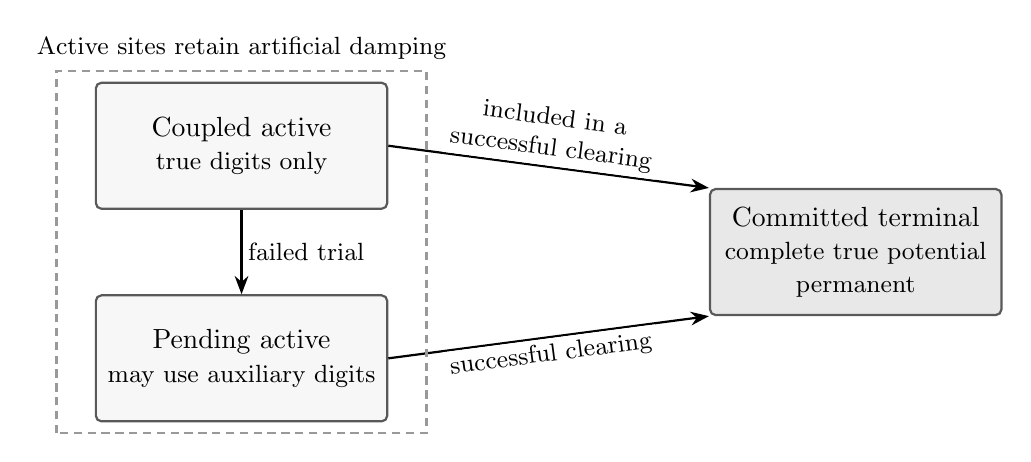
\begin{tikzpicture}[
  state/.style={draw=black!65,rounded corners=2pt,minimum width=37mm,
                minimum height=16mm,align=center,fill=black!3},
  lab/.style={font=\small,align=center,fill=white,inner sep=2pt},
  >=Stealth,thick]
\node[state] (coupled) at (0,1.35) {Coupled active\\\small true digits only};
\node[state] (pending) at (0,-1.35) {Pending active\\\small may use auxiliary digits};
\node[state,fill=black!9] (terminal) at (7.8,0) {Committed terminal\\\small complete true potential\\\small permanent};
\draw[->] (coupled) -- node[lab,right]{failed trial} (pending);
\draw[->] (pending.east) -- node[lab,below,sloped]{successful clearing} (terminal.south west);
\draw[->] (coupled.east) -- node[lab,above,sloped]{included in a\\successful clearing} (terminal.north west);
\draw[densely dashed,black!40] (-2.35,-2.30) rectangle (2.35,2.30);
\node[font=\small,anchor=south] at (0,2.32) {Active sites retain artificial damping};
\end{tikzpicture}

 \caption{The arrows show possible changes between committed site states.
 A pending mark is conservative: the marked site's own true suffix may
 remain unqueried. The final suffix sweep is reached only when no site is
 pending; after it succeeds, the active sites have complete true potentials
 and retain artificial damping.}
 \label{fig:site-states}
\end{figure}

Initially every site is active and coupled, and every partial value is
zero. The retained-information lemma below supplies the conditional law
of an unqueried input. Sections~\ref{sec:local-sweeps} and
\ref{sec:assembly} verify that the inputs selected by ordinary trials
and clearings are eligible for that law. In the matrix estimates,
``fresh'' means a centered variable with the stated law conditional on
the history available before the chosen update. It is an explicit input
until the corresponding eligibility check has been made.

\paragraph{Retained information.}
The construction uses a separate countable array of independent auxiliary
fair signs. It also uses independent uniform orders of fixed finite
sets: a uniform order of a set $S$ of size $M$ is a uniformly chosen
bijection from $\{1,\ldots,M\}$ to $S$. All these sources are independent
of the true signs and of one another. Only an auxiliary sign that is used,
or the next entry of an order being used, is exposed. Section~\ref{sec:local-sweeps}
specifies the source indices for each ordinary trial.

Number the successive queries and completed measurable decisions by
$q=1,2,\ldots$, and let
$\mathcal F_q^{\mathrm{ret}}$ be the information retained after operation $q$.
Initially $\mathcal F_0^{\mathrm{ret}}$ contains only the fixed parameters and deterministic
initial data. A completed measurable numerical choice counts as one
operation even when it is defined by a limit, as with the later ridge choice
or diagonal reset. Before a query, its type and source index are chosen
measurably from the current history. A query may expose one true digit,
one unused auxiliary sign, the remaining true suffix at a selected site,
or the next entry of a selected finite order that has an unexposed entry.
A whole true suffix is one
operation; under the fixed binary convention, its value determines all
the digits it contains. The history records the queried indices and
answers and every exposed order entry. Numerical updates, choices, and
failure decisions must be measurable from the information recorded by
that time, so adjoining them gives no further information.

The current potential values, active and terminal sets, pending marks, and
matrices are measurable functions of this retained history. Rollback and
marking are measurable operations, and the sigma-fields $\mathcal F_q^{\mathrm{ret}}$
continue to increase: answers observed in failed trials remain known.
Whenever an
operation installs an exact true value whose remaining digits have not
yet been queried, it first exposes and records that true suffix. This
also applies when the change is controlled by a deterministic estimate.

\begin{lemma}[Conditional freshness]\label{lem:conditional-freshness}
Suppose queries obey the preceding rule. Conditional on the retained
history, the unqueried true digits retain their product fair-sign law.
The same holds jointly for unused auxiliary signs. In particular, at
distinct sites whose remaining true suffixes are unqueried, those suffixes
are conditionally independent and have the uniform laws specified above.
After a revealed prefix of an independent uniform order, its remaining
order is conditionally uniform over the unexposed elements, jointly with
the stated product law for unqueried signs.

These statements hold after every deterministic finite number of
operations and at every almost surely finite stopping time of
$(\mathcal F_q^{\mathrm{ret}})$, with conditioning on the stopped sigma-field.
\end{lemma}

\begin{proof}
Condition on the history before a query. Its source index is then fixed.
Coordinates whose values are already recorded contribute no new
information. If a query includes both known and unqueried digits, apply
the following factorization to its unqueried part.
For a sign query, the product law factors into the queried coordinate and
the other unqueried coordinates. Adjoining the answer leaves the latter
factors unchanged. For a whole true suffix, apply the same argument to
its block of digits: test against finite cylinder functions of the other
coordinates and then use the monotone class theorem. This is a statement
about conditional expectations, so it also covers a continuous residual
answer without conditioning on an individual value of probability zero.
The same factorization applies to unused auxiliary signs.

For a uniform order with $r$ elements still unexposed, each possible
next element has exactly $(r-1)!$ completions. Its remaining order is
therefore uniform after that entry is revealed. An answer subsequently
queried at the selected index uses no unexposed order entry. Choices and
failure decisions made from the enlarged history add no information.
Induction proves the assertions after every fixed finite number of
operations.

For precision at a random operation time, let $\tau$ be a stopping time
of $(\mathcal F_q^{\mathrm{ret}})$ with $\PP(\tau<\infty)=1$, and let $\mathcal F_\tau^{\mathrm{ret}}$
be its stopped sigma-field. For $D\in\mathcal F_\tau^{\mathrm{ret}}$, apply each
finite-operation conditional-expectation identity against
$D\cap\{\tau=q\}\in\mathcal F_q^{\mathrm{ret}}$ and sum over $q$. These countably many
events exhaust $D$ up to a null set and give the same identity conditional
on $\mathcal F_\tau^{\mathrm{ret}}$. A whole-suffix query remains one operation in this
argument.
\end{proof}

\subsection{Schur reduction and the Ward Laplacian}

For the fixed $E$ and $\lambda>0$, almost surely every principal matrix
of the true $H_m-E$ is invertible. Indeed, for a nonempty subset its
determinant is a polynomial in the independent continuous potentials,
with nonzero highest monomial $\prod_{i}\lambda V_i$. Its zero set has
Lebesgue measure zero. There are finitely many subsets on the torus.
We henceforth work on this event, which also covers subsets chosen
adaptively later. This probability-one property is not a preliminary
test of unrevealed potentials and supplies no information to the
algorithm's filtration. The empty terminal block requires no inverse.

Let $\mathcal H$ be the real symmetric matrix with the current real
potential values on $A$ and exact true values on $T$. Eliminate the terminal
block at the real energy $E$, obtaining
\[
 M=(\mathcal H-E)_{AA}
   -(\mathcal H-E)_{AT}(\mathcal H-E)_{TT}^{-1}
                         (\mathcal H-E)_{TA}.
\]
The matrix $M$ is real symmetric. Its off-diagonal entries connect
nearest neighbors or sites joined through one connected component
of terminal sites. Throughout, the subscript in a Schur complement
names the \emph{eliminated} indices: if $R$ is the complement of $\mathcal E$,
\[
 \Schur_{\mathcal E} B
 =B_{RR}-B_{R\mathcal E}B_{\mathcal E\mathcal E}^{-1}B_{\mathcal ER}.
\]
We use this notation only when the displayed inverse exists.
Put $r=(r_i)_{i\in A}\in\CC^A$, $p_i=\Im r_i>0$,
and, for a scale $t>0$, define
\[
 g=(M-t\diag r)^{-1},\qquad h=\sqrt t\,g,\qquad
 K_{ij}=h_{ij}^2,\quad F_{ij}=|h_{ij}|^2,\quad q_i=\Im g_{ii}.
\]
The inverse exists because its matrix has strictly negative imaginary
part. In particular $\|g\|\le(t\min p_i)^{-1}$.
Both $g$ and $h$ are complex symmetric. For a matrix $B$,
$\Im B=(B-B^*)/(2i)$; here it is also the entrywise imaginary part.
The resolvent identity gives the Ward identity
\begin{equation}\label{eq:ward}
 h\diag(p)h^*=\Im g,\qquad Fp=q.
\end{equation}
Consequently
\[
 D=\diag(pq)-\diag(p)F\diag(p)
\]
is a real graph Laplacian, with nonnegative edge weights
$p_i p_jF_{ij}$. Its quadratic form is
\[
 D(f)=\frac12\sum_{i,j}p_i p_jF_{ij}|f_i-f_j|^2.
\]
The nonnegative weights $F_{ij}=|h_{ij}|^2$ describe how the Ward mass is
distributed across a row.
We use $B(f)=\langle f,Bf\rangle$ for the quadratic form of a Hermitian
matrix. At the committed states below, the kernel of $D$ is precisely
the constants. Its pseudoinverse $X=D^+$ is then an inverse on neutral
charges, namely vectors $y$ with $\sum_i y_i=0$.

We record the precise Schur identity for these inverse forms. If
$U$ is eliminated and $R=A\setminus U\ne\varnothing$, then $D_{UU}$
is positive definite: extending a zero-energy vector by zero on $R$
would otherwise give a nonconstant vector in $\ker D$. Moreover,
\[
 (\Schur_U D)(f_R)=\min_{f_U}D(f_R,f_U).
\]
It follows that $\Schur_U D$ has only the constant kernel. For a
neutral $y$ supported on $R$, extend it by zero to $A$ and use the
variational formula
\[
 X(y)=\sup_f\{2\Re\langle y,f\rangle-D(f)\}.
\]
Minimizing first over $f_U$ proves
\begin{equation}\label{eq:schur-inverse-form}
 (\Schur_U D)^+(y)=D^+(y).
\end{equation}
All later inverse-form comparisons across deletion are understood in
this sense, on survivor-supported neutral charges, not as an equality
of full pseudoinverse matrices.

At the beginning of a stage the state satisfies $r_i=g_{ii}$.
During a sweep or clearing trial, $r$ remains frozen. Thus $q=p$
at the stage boundary, and the difference $g_{ii}-r_i$ measures the
subsequent diagonal lag. Because $g$ itself depends on $r$, restoring
the equality requires a small self-consistent correction. The stage-end
reset in Section~\ref{sec:assembly} constructs that correction.

The role of $K$ is visible in this self-consistency equation. For the
physical active inverse, differentiation with respect to the complex
diagonal parameter gives
\[
 \frac{\partial g_{ii}}{\partial r_j}=t g_{ij}^2=K_{ij}.
\]
Thus the linearization of $r-(g_{ii}(r))_{i\in A}=0$ is $\Id-K$, which is
invertible whenever $\|K\|<1$.

For $n_0\le n<m$, a transition from scale $n$ to $n+1$ consists of an
ordinary sweep, any scheduled clearings at $t_{n+1}$, and a diagonal reset.
Clearings run only through $J=\lfloor m/2\rfloor$. At the end of stage $J$,
the construction aborts if any site remains pending; after $J$ it aborts
if the first trial at any tile fails. At scale $m$, a final residual sweep
inserts each remaining true suffix, leaves damping $\eta$, and has no reset.
Sections~\ref{sec:assembly} and~\ref{sec:history} specify the trial, marking,
and abort rules.

\subsection{The bounds carried between stages}

The full-torus positive nearest-neighbor Laplacian is denoted by
$\Lambda$. Thus $\Lambda(v)$ is the sum of $|v_i-v_j|^2$ over unordered
nearest-neighbor edges. Charges on a subset are extended by zero when
inserted in $\Lambda^+$. We fix
\[
 \delta=0.01,\qquad \kappa=0.005\delta,\qquad
 \nu=10^{-5}\delta/d,\qquad H_*=t^{1+\delta},\qquad b=t_{n_0}t.
\]
Thus $d\nu=10^{-5}\delta$; the dimension-scaled choice will absorb the
overlap of component neighborhoods. Constants in $O(\cdot)$ depend
only on $d$, the displayed fixed energy window, and the fixed broad
bounds specified below. By making $\lambda_0(d)$
smaller we may make $n_0$ arbitrarily large. Every later use of a strict
power margin is made after this single choice.

At a committed stage boundary, the entries of $r$ are bounded and
$c\le p_i\le C$. We maintain
\[
 \|K\|\le\tfrac13,\qquad
 \max_i\sum_j|h_{ij}|^4\le H_*,\qquad \ker D=\CC\mathbf1.
\]
The fourth-power bound is the squared row norm $\sum_jF_{ij}^2$.
It limits concentration across the columns of each row. The local
variance estimates need this control in addition to Ward's bound on
the weighted row sum.
On neutral charges we maintain the three comparisons
\begin{equation}\label{eq:comparators}
 \begin{aligned}
 X&\ge c_n b\,\Lambda^+,\\
 X&\le C_0\Id+C_n b\,\Lambda^+,\\
 X&\le(1+t^\kappa)\diag(p^{-2})+C_n t\,\Lambda^+.
 \end{aligned}
\end{equation}
Here $C_0$ is a sufficiently large fixed constant, while $c_n,C_n$
remain bounded above and below by positive constants, changing only
by summable relative errors. Boundedness of the weighted row sums of
$F$ also gives $X\ge c\Id$ on this subspace: the absolute row sums
of $D$ are at most $2\max_i p_iq_i$, so $D\le C\Id$.

The first two comparisons express an equivalence of spatial energies.
To formulate it also for the duplicated sites used in a sweep, allow
one or two \emph{ports} at each active physical site. For a port charge
$y$, let $y_\Sigma$ be the full-torus charge formed by summing its ports
at each physical site and extending by zero. A full-torus function $v$
is repeated at all ports at a site. Define the dual quadratic forms
\begin{equation}\label{eq:dual-forms}
 \begin{aligned}
 W^*(y)&=\|y\|_2^2+b\,\Lambda^+(y_\Sigma),\qquad \sum_x y_x=0,\\
 W(f)&=\inf_{f=\alpha+v|_{\mathrm{ports}}}
       \left(\|\alpha\|_2^2+b^{-1}\Lambda(v)\right).
 \end{aligned}
\end{equation}
The second form is on potentials modulo constants.
Lemma~\ref{lem:dual-forms} proves the duality and explains the resulting
relations $X\asymp W^*$ and $D\asymp W$. The final comparison in
\eqref{eq:comparators} is sharper: its high-frequency diagonal
coefficient tends to one. Retaining that coefficient will supply the
extra gain in the row-fourth-moment estimates.

We also track geometry. Let $d_T(i,j)$ be shortest-path pseudodistance in the
physical torus when an edge touching a terminal site has cost zero
and every other nearest-neighbor edge has cost one. The induction
will maintain
\[
 d_T(i,j)\ge\tfrac12\dist(i,j)-t^{-1.03}.
\]
The matrices $M$ can have large entries after a Schur reduction.
Nevertheless, every nonlocal entry joins points at zero $d_T$-distance.
This permits the resolvent decay estimate needed for local monitoring.
Section~\ref{sec:assembly} proves the geometric bound, including the
temporary terminal sites inside a clearing trial.

There are two distinct uses of these bounds. An ordinary trial stops at
the first local budget violation or failure of a required prefix bound,
including the global correction, row, and lag caps. The violating increment
is included in the stopped estimates.
Clearing prefixes are governed by their own stopped trial budgets, which
yield the provisional diagonal and row bounds; geometry is supplied
separately. For each
successful clearing, the assembly argument proves the $K$ and Laplacian
comparisons for the committed output from its stated hypotheses. The
trial statements make these two regimes explicit. The maximal
concentration estimate used for their stopped probability bounds is
proved in Section~\ref{sec:local-sweeps}.

\section{The initial state and its comparison forms}
\label{sec:initialization}

This section constructs the initial state with every site active and its
partial potential equal to zero, for every fixed $d\ge3$ and the
corresponding interval $I_d$ in \eqref{eq:energy-windows}. We prove that the initial inverse has a
bounded diagonal, a small squared-entry operator, small fourth-power row
sums, and the three comparison bounds in \eqref{eq:comparators}. We first establish the lattice
inequalities used to express those bounds and to localize them later.

\subsection{Duality and lattice estimates}

Let $\mathbb T_L=(\ZZ/L\ZZ)^d$, $L\ge4$, and $N=L^d$. An index set
$\mathcal A$ consists of sites of $\mathbb T_L$, with at most two copies
of each site permitted.  Write $\pi:\mathcal A\to\mathbb T_L$ for the
underlying site map.  For a function $v$ on $\mathbb T_L$, let
$(\mathcal Cv)_x=v_{\pi(x)}$.  The adjoint sends a charge $y$ on
$\mathcal A$ to
\[
 (y_\Sigma)_i=(\mathcal C^*y)_i
 =\sum_{x:\pi(x)=i}y_x,
\]
with value zero at sites not represented in $\mathcal A$.
The positive nearest-neighbor Laplacian is denoted by $\Lambda$, and
$\Lambda^+$ is its inverse on mean-zero functions, extended by zero on
constants.  We normalize the gradient energy by
$\|\nabla v\|_2^2=\langle v,\Lambda v\rangle$.

\begin{lemma}[Dual comparison forms]\label{lem:dual-forms}
For $b>0$, define
\[
 \begin{split}
 W(f)&=\inf_{f=\alpha+\mathcal Cv}
       \bigl(\|\alpha\|_2^2+b^{-1}\|\nabla v\|_2^2\bigr),\\
 W^*(y)&=\|y\|_2^2+
       b\langle y_\Sigma,\Lambda^+y_\Sigma\rangle,
       \qquad \sum_{x\in\mathcal A}y_x=0.
 \end{split}
\]
Then $W$ is a positive definite quadratic form on functions on
$\mathcal A$ modulo constants, and $W^*$ is its dual quadratic form:
\[
 W^*(y)=\sup_f\bigl(2\Re\langle y,f\rangle-W(f)\bigr).
\]
In particular, if $D$ is a Laplacian on $\mathcal A$ whose kernel is
exactly the constants and $X=D^+$, then
$cW^*\le X\le CW^*$ on neutral charges is equivalent to
$C^{-1}W\le D\le c^{-1}W$ on functions modulo constants.
\end{lemma}

\begin{proof}
Because $\mathcal C$ carries constants to constants, $W$ is unchanged by
addition of a constant to $f$.  The minimization is a finite-dimensional
least-squares problem, so its minimum is attained and is a quadratic
form in $f$.  Zero energy forces $\alpha=0$ and $v$
constant, so the induced form on the quotient is positive definite.

For a neutral $y$, completion of squares gives
\[
\begin{split}
 \sup_f\bigl(2\Re\langle y,f\rangle-W(f)\bigr)
 &=\sup_{\alpha,v}\bigl(
       2\Re\langle y,\alpha+\mathcal Cv\rangle
       -\|\alpha\|_2^2-b^{-1}\langle v,\Lambda v\rangle\bigr)\\
 &=\|y\|_2^2+b\langle\mathcal C^*y,
                         \Lambda^+\mathcal C^*y\rangle.
\end{split}
\]
Neutrality makes $\mathcal C^*y$ orthogonal to constants.  The inverse
matrix of a positive quadratic form is its dual, which proves both the
identity and the comparison assertion on the quotient.
\end{proof}

We use unnormalized Fourier coefficients
$\widehat y(k)=\sum_x y_xe^{-ik\cdot x}$, with inverse normalization
$N^{-1}$.  Frequencies belong to the grid
$\mathcal K_L=(2\pi/L)\ZZ^d$ modulo $2\pi\ZZ^d$, represented in
$[-\pi,\pi)^d$; the symbol of
$\Lambda$ is
\begin{equation}\label{eq:initial-laplacian-symbol}
 \ell(k)=4\sum_{j=1}^d\sin^2(k_j/2)\asymp |k|^2.
\end{equation}

\begin{lemma}[A charge estimate for fixed dimension $d\ge3$]
\label{lem:fourier-charge}
There is a constant $C_d$ such that, for every $L\ge4$, every index
set $\mathcal A$ as above, and every charge $y$ on $\mathcal A$,
\[
 \langle y_\Sigma,\Lambda^+y_\Sigma\rangle
 \le C_d\|y\|_1^{4/3}\|y\|_2^{2/3}.
\]
\end{lemma}

\begin{proof}
Counting grid frequencies in dyadic annuli and using
\eqref{eq:initial-laplacian-symbol} gives
\begin{equation}\label{eq:initial-frequency-sum}
 N^{-1}\sum_{0<|k|\le a}\ell(k)^{-1}
 \le C_d a^{d-2}\le C_d a,
 \qquad 0<a\le1.
\end{equation}
For completeness, a ball of radius $r\ge2\pi/L$ contains at most
$C_d(1+Lr)^d\le C_dNr^d$ grid points. On an annulus
$r/2<|k|\le r$, the summand is at most $C r^{-2}$. Decomposing the
ball of radius $a$ into dyadic annuli, discarding empty annuli below
the first mesh frequency, gives
$C_d\sum_{j\ge0}(2^{-j}a)^{d-2}\le C_da^{d-2}$.
If $a$ is smaller than the first nonzero frequency, the sum is empty.
The weaker last bound deliberately retains the exponents needed later;
it is valid because $a\le1$ and $d-2\ge1$.

At each frequency $|\widehat{y_\Sigma}(k)|\le\|y\|_1$, while at most
two copies per site gives $\|y_\Sigma\|_2^2\le2\|y\|_2^2$.
The low frequencies in the quadratic form are therefore bounded by
$Ca\|y\|_1^2$, and Parseval bounds the high frequencies by
$Ca^{-2}\|y\|_2^2$.  For $y\ne0$, choose
$a=(\|y\|_2/\|y\|_1)^{2/3}\le1$.  This proves the claimed
inequality.  For $y=0$ there is nothing to prove.
\end{proof}

\begin{lemma}[Weighted cube inequality]\label{lem:cube-weight}
Let $Q$ be a lattice cube in $\ZZ^d$ of integer side $l\ge1$,
let $v:Q\to\CC$, and let $w_i\ge0$ be weights. With the gradient
restricted to edges contained in $Q$,
\[
 \|v-\operatorname{avg}_Qv\|_{2,Q}^2
 \le C_d l^2\|\nabla v\|_{2,Q}^2,
\]
and
\begin{equation}\label{eq:initial-weighted-cube}
 \sum_{i\in Q}w_i|v_i-\operatorname{avg}_Qv|^2
 \le C_d(\max_Q w)^{1/3}\Bigl(\sum_Qw\Bigr)^{2/3}
          \|\nabla v\|_{2,Q}^2.
\end{equation}
For fixed $d$, the constants are independent of $l$, $v$, and the
weights. The statements also hold for cubes in a torus whenever their
internal edges are identified with those of a lattice cube.
\end{lemma}

\begin{proof}
The case $l=1$ is immediate. Translate $Q$ to
$\{0,\ldots,l-1\}^d$. Define
\[
 \rho(j)=
 \begin{cases}j,&0\le j<l,\\2l-1-j,&l\le j<2l,\end{cases}
 \qquad
 V(j_1,\ldots,j_d)=v(\rho(j_1),\ldots,\rho(j_d))
                         -\operatorname{avg}_Qv.
\]
This gives a centered function on $\mathbb T_{2l}$. Each original site
has $2^d$ preimages. Every internal cube edge is copied $2^d$ times,
and differences on the folding edges vanish. Consequently
\[
 \|V\|_2^2=2^d\|v-\operatorname{avg}_Qv\|_{2,Q}^2,
 \qquad \Lambda_{2l}(V)=2^d\|\nabla v\|_{2,Q}^2.
\]
The smallest positive eigenvalue of $\Lambda_{2l}$ is at least
$c l^{-2}$, so Parseval proves the first assertion.

For the weighted assertion put $M=\max_Q w$ and $S=\sum_Qw$.
If $S=0$ there is nothing to prove. Otherwise
$a=(M/S)^{1/3}\in(0,1]$. Split $V$ into frequencies $0<|k|\le a$
and $|k|>a$; its zero Fourier coefficient vanishes. With normalized
inverse Fourier transformation, Cauchy--Schwarz gives
\[
 |V_{\rm low}(x)|^2
 \le\left((2l)^{-d}\sum_{0<|k|\le a}\ell(k)^{-1}\right)
       \left((2l)^{-d}\sum_k\ell(k)|\widehat V(k)|^2\right).
\]
Thus \eqref{eq:initial-frequency-sum} and Parseval imply
\[
 \|V_{\rm low}\|_\infty^2\le C_d a\Lambda_{2l}(V),
 \qquad
 \|V_{\rm high}\|_2^2\le C_d a^{-2}\Lambda_{2l}(V).
\]
These inequalities include the case of an empty low-frequency range.
Restricting to $Q$, using $|z_1+z_2|^2\le2|z_1|^2+2|z_2|^2$,
and applying the exact reflection identities above, we obtain
\[
 \sum_{i\in Q}w_i|v_i-\operatorname{avg}_Qv|^2
 \le C_d(Sa+Ma^{-2})\|\nabla v\|_{2,Q}^2.
\]
The chosen value of $a$ gives
$Sa=Ma^{-2}=M^{1/3}S^{2/3}$, proving the claim.
\end{proof}

\begin{lemma}[Spatial counting and exponential moments]
\label{lem:lattice-counting}
For ordinary nearest-neighbor distance on $\mathbb T_L$, balls satisfy
$|B(x,R)|\le C_d(1+R)^d$. If $1\le R\le L/4$, they also satisfy
$|B(x,R)|\ge c_dR^d$. Uniformly in $L$, for $0<u\le1$ and $a=0,2$,
\begin{equation}\label{eq:lattice-exponential-moments}
 \sum_y\dist(x,y)^a e^{-u\dist(x,y)}\le C_d u^{-d-a},
\end{equation}
where the factor $\dist(x,x)^0$ is interpreted as $1$.
\end{lemma}

\begin{proof}
Represent each displacement by coordinate differences of least
absolute value. A distance ball is contained in the coordinate box
$[-R,R]^d$, proving the upper bound. For $R\le L/4$, a coordinate
box of radius $\lfloor R/d\rfloor$ embeds without identifications
and is contained in the distance ball, giving the lower bound after
adjusting the constant for bounded $R$. The number of representatives
at distance $r$ is at most $C_d(1+r)^{d-1}$, by counting nonnegative
integer $d$-tuples of sum $r$ and their signs. Thus the left side of
\eqref{eq:lattice-exponential-moments} is bounded by
$C_d\sum_{r\ge0}(1+r)^{d-1+a}e^{-ur}$, which is at most
$C_du^{-d-a}$ by comparison with its integral.
\end{proof}

These lattice estimates are uniform in the torus and cube sizes.
They will allow local changes to be measured in the same forms as the
initial state.  We now construct that state and identify its Fourier
comparison operator.

\subsection{The fixed interval and the scalar diagonal equation}

Self-consistent diagonal equations and free lattice resolvent estimates
also play a central role in
\cite[Section~2.2 and Appendix~A]{BlackDroginHernandez2025}.
We prove the specific finite-volume estimates needed here, including
the gap at the smallest nonzero grid frequency.

The free dispersion in the negative-hopping convention is
\[
 a(k)=-2\sum_{j=1}^d\cos k_j=-2d+\ell(k).
\]
Write $a_d=e_2$ for $d=3$ and $a_d=1/100$ for $d\ge4$, so that
$I_d=-2d+(a_d/2,a_d)$. Choose $e_2>0$ fixed and sufficiently small,
with $e_2<1/100$. For estimates involving a small shift of energy,
use the larger compact offset interval
\[
 \mathcal J_d=[2a_d/5,5a_d/4]\subset(0,0.04).
\]
For $d\ge4$ this is exactly $[1/250,1/80]$.
The parameter $a_d$ is fixed before the coupling or any scale is chosen.
In the free-resolvent analysis below, constants may depend on $d$ and this
fixed $a_d$; this dependence is included in the notation $C_d$.
In what follows, integrals over the frequency torus are
normalized by $(2\pi)^{-d}$.

\begin{lemma}[The free resolvent near the band minimum]
\label{lem:initial-bottom-density}
The function
\[
 G_0(z)=\int_{[-\pi,\pi)^d}\frac{1}{a(k)-z}\,
                    \frac{dk}{(2\pi)^d},\qquad \Im z>0,
\]
extends continuously from above to $-2d+\mathcal J_d$. Its boundary imaginary
part there is bounded above and below by positive constants depending
only on the fixed dimension and window. Uniformly for
$\alpha\in-2d+\mathcal J_d$ and $0<v\le1$,
\begin{equation}\label{eq:initial-density-integrals}
 \int\frac{dk/(2\pi)^d}{|a(k)-\alpha-iv|}
       \le C_d\log(2/v),
 \qquad
 \left|\int\frac{dk/(2\pi)^d}{(a(k)-\alpha-iv)^2}\right|
       \le C_d\log(2/v).
\end{equation}
The second estimate holds uniformly also for
$-2\sum_{j=1}^dc_j\cos(k_j+\phi_j)$ whenever
$\max_j|c_j-1|\le\varepsilon_d$ for a sufficiently small fixed
$\varepsilon_d>0$, with arbitrary real phases $\phi_j$.
\end{lemma}

\begin{proof}
On $(-\pi,\pi)^d$ make the one-to-one change of coordinates
$x_j=2\sin(k_j/2)$. Then $a(k)+2d=|x|^2$ and
$dk=\prod_j(1-x_j^2/4)^{-1/2}dx$. For $0<s<0.04$ the entire
sphere of radius $\sqrt s$ lies in the coordinate domain, so polar
integration shows that the normalized density of $a+2d$ equals
\begin{equation}\label{eq:initial-density-formula}
 \rho_d(s)=\frac{s^{d/2-1}}{2(2\pi)^d}
   \int_{S^{d-1}}\prod_{j=1}^d
       (1-s\omega_j^2/4)^{-1/2}\,d\sigma(\omega).
\end{equation}
This density is positive and smooth on $(0,0.04)$. On every compact
subinterval its derivatives are bounded and the density has a positive
lower bound, with constants allowed to depend on $d$.

Choose a smooth cutoff $\chi$ supported in $(a_d/5,2a_d)$ and equal
to one on a neighborhood of $\mathcal J_d$. Split the Stieltjes integral into
this localized density and the complementary part. In the latter
part the real denominator stays a fixed distance from zero for
energies in $-2d+\mathcal J_d$, so it is continuous and bounded up to the real
axis, as is its derivative. In the former part, subtract
$\rho_d(\alpha+2d)$ locally from the density. The difference vanishes
linearly at the real energy; its Cauchy integral has a continuous
upper boundary value. The constant part is an explicit logarithmic
integral. This proves upper-half-plane continuity and gives the
boundary imaginary part $\pi\rho_d(\alpha+2d)$.

For the first inequality in \eqref{eq:initial-density-integrals},
integrate the bounded localized density against
$((s-(\alpha+2d))^2+v^2)^{-1/2}$; its integral over the fixed support
is at most $C\log(2/v)$. For the second, integration by parts gives
\[
 \int\frac{\chi(s)\rho_d(s)}{(s-(\alpha+2d)-iv)^2}\,ds
 =\int\frac{(\chi\rho_d)'(s)}{s-(\alpha+2d)-iv}\,ds.
\]
There is no boundary term. The same absolute-integral estimate bounds
this expression, while the complementary contribution stays bounded.

For the perturbation assertion, first translate all phases in the
continuum torus integral. Put
$x_j=2\sqrt{c_j}\sin(k_j/2)$, so the new minimum is
$-2\sum_jc_j$ and the excess energy is $|x|^2$. The Jacobian is
\[
 \prod_{j=1}^d c_j^{-1/2}
            (1-x_j^2/(4c_j))^{-1/2}.
\]
Choose $\varepsilon_d$ so small that $c_j\ge1/2$ and
$2d\varepsilon_d<a_d/10$. Energies in $-2d+\mathcal J_d$ then have excess
above the shifted minimum in a fixed compact subinterval of
$(a_d/5,2a_d)$. The corresponding polar density and its derivatives
are uniformly bounded there. A cutoff equal to one on that compact
interval gives the same integration-by-parts estimate, uniformly in
the coefficients and phases.
\end{proof}

\begin{proposition}[Initialization]\label{prop:initialization}
For each fixed $d\ge3$ there are $\lambda_0(d)>0$ and positive
constants $a_0,B,c,C,C_0$, depending only on the fixed dimension and
window, with the following
property.  For
$0<\lambda<\lambda_0(d)$, the scales in \eqref{eq:scales},
$m\ge4n_0$, $L=4^{20m}$, and every $E\in I_d$,
write $t=t_{n_0}$.  There is a scalar $r$ with
\[
 |\Re r|\le B,\qquad a_0\le p:=\Im r\le B,
 \qquad
 r=N^{-1}\sum_k\frac1{a(k)-E-tr}.
\]
It is the unique solution in the displayed rectangle and depends
continuously on $E$.

Take all sites active, all partial potentials zero, and
$g=(H_0-E-tr)^{-1}$, where $H_0$ is the free hopping matrix on
$\mathbb T_L$.  With $h,K,F,D,X$ as in
Section~\ref{sec:state}, one has $g_{ii}=r$, $\|K\|\le1/10$, and
\[
 \max_i\sum_j|h_{ij}|^4\le\tfrac1{10}t^{1+\delta}.
\]
The kernel of $D$ is exactly the constants, and on neutral charges,
\begin{equation}\label{eq:initial-comparisons}
 \begin{split}
 X&\ge ct^2\Lambda^+,\qquad X\ge c\Id,\\
 X&\le C_0\Id+Ct^2\Lambda^+,\\
 X&\le(1+t^\kappa)p^{-2}\Id+Ct\Lambda^+.
 \end{split}
\end{equation}
Thus this state satisfies \eqref{eq:comparators}, with startup
$b=t_{n_0}t=t^2$ and constants independent of $E,\lambda,m$.
\end{proposition}

\begin{proof}
We first solve the scalar equation, then prove the two smallness bounds,
and finally identify the inverse form of $D$.

\paragraph{The scalar fixed point.}
By Lemma~\ref{lem:initial-bottom-density}, the boundary values
$G_0(\alpha+i0)$ for $\alpha\in-2d+\mathcal J_d$ form a compact subset
of the upper half-plane. Choose $a_0>0$ and $B<\infty$ so that they lie
strictly inside the rectangle
\[
 \mathcal B=\{r:|\Re r|\le B,\ a_0\le\Im r\le B\}.
\]
The closure of $I_d$ lies in the interior of $-2d+\mathcal J_d$.
Hence, when $t$ is small, $E+t\Re r\in-2d+\mathcal J_d$ for every
$E\in I_d$ and $r\in\mathcal B$. Uniform boundary continuity on this
compact interval shows that $r\mapsto G_0(E+tr)$ maps $\mathcal B$
into its interior with fixed slack.

For a periodic $C^1$ function, comparing each grid cell with its corner
gives an integral-to-grid error at most $CL^{-1}\|\nabla f\|_\infty$.
On $\mathcal B$, set $z=E+tr$ and $R(k)=(a(k)-z)^{-1}$.
Since $\Im z\asymp t$,
\begin{equation}\label{eq:initial-grid-derivatives}
 \|\nabla R\|_\infty\le Ct^{-2},\qquad
 \|\nabla(R^2)\|_\infty\le Ct^{-3}.
\end{equation}
The finite-grid map
$\Phi(r)=N^{-1}\sum_kR(k)$ consequently preserves $\mathcal B$,
provided $C/(Lt^2)$ is sufficiently small.  Here
$t\asymp4^{-n_0}$ and $L\ge4^{20n_0}$, so
\begin{equation}\label{eq:initial-grid-error}
 \varepsilon_L:=\frac{C}{Lt^2}\le Ct^{18}.
\end{equation}

The second estimate of Lemma~\ref{lem:initial-bottom-density} holds for
every $r\in\mathcal B$, without a fixed-point hypothesis.  Differentiating
the finite sum and using \eqref{eq:initial-grid-derivatives} gives
\[
 \sup_{r\in\mathcal B}|\Phi'(r)|
 \le Ct\log(1/t)+\varepsilon_L.
\]
It is less than $1/2$ for small $t$.  Integrating the complex derivative
along any segment in the convex rectangle makes $\Phi$ a contraction.
Iteration from one fixed starting point in $\mathcal B$ constructs its unique
fixed point.  The iterates are continuous in $E$ and converge uniformly,
so the fixed point is continuous in $E$.

At this solution, translation invariance gives $g_{ii}=r$.  Taking
imaginary parts of the scalar equation, and cancelling $p>0$, yields
the exact finite-grid normalization
\begin{equation}\label{eq:initial-normalization}
 t\operatorname{avg}_k|R(k)|^2=1.
\end{equation}

\paragraph{The Fourier symbols and the remaining bounds.}
For each grid displacement $\zeta\in\mathcal K_L$, Fourier transformation gives
\begin{equation}\label{eq:initial-symbols}
 \widehat F(\zeta)
    =t\operatorname{avg}_k R(k)\overline{R(k+\zeta)},\qquad
 \widehat K(\zeta)
    =t\operatorname{avg}_k R(k)R(k+\zeta).
\end{equation}
The first symbol is real, either because $F$ is real and even or by
the change $k\mapsto-k-\zeta$ and $R(-k)=R(k)$. Its zero mode is
$1$ by \eqref{eq:initial-normalization}, and Cauchy--Schwarz gives
$|\widehat F(\zeta)|\le1$. Both convolution operators are unitarily
diagonalized by Fourier transformation, and Parseval gives the row identity:
\[
 \|K\|=\max_{\zeta\in\mathcal K_L}|\widehat K(\zeta)|,\qquad
 \sum_j|h_{ij}|^4
   =N^{-1}\sum_{\zeta\in\mathcal K_L}|\widehat F(\zeta)|^2.
\]
Thus the two smallness assertions require a uniform bound for
$\widehat K$ and an averaged square bound for $\widehat F$.
At the fixed point $q=p$ is scalar, so $D=p^2(\Id-F)$.
The inverse-form comparisons will follow from a two-sided estimate of
$1-\widehat F(\zeta)$ at every nonzero grid frequency. At higher
frequencies we will also use that $\widehat F$ is small to retain the
sharp diagonal coefficient.

\paragraph{An absolute-product bound, including tangential intersections.}
We first pass to the continuum frequency torus. For every nonzero
displacement $\zeta\in[-\pi,\pi)^d$, we claim
\begin{equation}\label{eq:initial-absolute-product}
 t\int |R(k)R(k+\zeta)|\,\frac{dk}{(2\pi)^d}
 \le\frac{C_dt\log^2(1/t)}{|\zeta|}.
\end{equation}
For quadratic dispersion, Erd\H{o}s, Salmhofer and Yau obtain a related
inverse-displacement two-resolvent bound by radial and angular integration
\cite[author-preprint Appendix~A, Lemma~A.1, equations~(A.2) and~(A.4)]{ErdosSalmhoferYau2008}.
The proof below supplies the required near-bottom lattice estimate by
convex slicing, including tangency.

In this estimate the displacement need not lie on the finite grid.
For small $t$ the real excess energy $\Re z+2d$ lies in $\mathcal J_d$.
If either dispersion has excess at least $0.04$, the corresponding
denominator is separated from zero by a fixed positive constant.
Lemma~\ref{lem:initial-bottom-density} then bounds this part of the
integral, including the factor $t$, by $C_dt\log(1/t)$. This is
absorbed by the right side of \eqref{eq:initial-absolute-product},
since $|\zeta|\le\pi\sqrt d$.

In the joint region where both excess energies are below $0.04$,
the frequency vectors $k$ and $k+\zeta$ have unique small unwrapped
representatives: every coordinate has absolute value at most
$2\arcsin(0.1)<0.201$. Their difference is the representative
$\zeta$, so $|\zeta_j|<0.402$. Set
$x_j=\sin(k_j+\zeta_j/2)$. The joint region is contained in
$|x_j|<1/4$, where the change of variables and its inverse have bounded
Jacobians. The two dispersions become
\[
 A_\pm(x)=-2\sum_{j=1}^d\cos(\zeta_j/2)\sqrt{1-x_j^2}
             \ \pm\ 2\sum_{j=1}^d\sin(\zeta_j/2)x_j.
\]
Since $\cos(\zeta_j/2)\ge\cos(0.201)>0$, their Hessians are
uniformly positive and bounded on that box. Their
difference is linear:
\[
 A_+(x)-A_-(x)=b_\zeta\cdot x,
 \qquad (b_\zeta)_j=4\sin(\zeta_j/2),
 \qquad c|\zeta|\le|b_\zeta|\le C|\zeta|.
\]

Suppose that the two energy constraints
\[
 |A_-(x)-\Re z|\le s_1,\qquad |A_+(x)-\Re z|\le s_2
\]
hold simultaneously, where $s_1,s_2>0$. Their difference gives
$|b_\zeta\cdot x|\le s_1+s_2$. Thus $x$ lies in a slab normal to
$b_\zeta$ of width at most $C\max(s_1,s_2)/|\zeta|$. On each slice
of this slab, the remaining task is to bound the narrower energy shell,
including when the slice is tangent to an energy surface.

For either sign, every affine hyperplane $H$ meeting the box, every
$E'\in\RR$, and every $s>0$, we claim
\[
 \operatorname{vol}_{H}\bigl\{x\in H\cap[-1/4,1/4]^d:
             |A_\pm(x)-E'|\le s\bigr\}\le C_ds,
\]
where $\operatorname{vol}_{H}$ is $(d-1)$-dimensional volume on $H$.
Fix the sign and extend each one-variable summand outside its
coordinate interval by its second-order Taylor quadratic at the
endpoint. This gives a globally $C^2$ function $f$ with
$c\Id\le\nabla^2f\le C\Id$, uniformly in $\zeta$. On a hyperplane
$H$ that meets the box choose $x_0\in H$ in the box. The restriction
$f|_H$ is coercive and uniformly convex, and therefore has a unique
minimizer $x_*$. If $P_H$ is projection to the direction space of $H$,
strong convexity and $P_H\nabla f(x_*)=0$ give
\[
 c|x_*-x_0|\le |P_H\nabla f(x_0)|\le C_d.
\]
Consequently $H$ intersected with the box lies in a ball of a fixed
radius $R_d$ about $x_*$. In polar coordinates in $H$, of dimension
$q=d-1\ge2$, one has
\[
 \frac{d}{dr}f(x_*+r\omega)\ge cr,
 \qquad
 \frac{r^{q-1}}{\frac{d}{dr}f(x_*+r\omega)}
       \le C r^{q-2}\le C_d\quad(0<r\le R_d).
\]
Along each ray the energy is increasing. Changing from $r$ to the
energy and integrating an interval of length $2s$ proves the asserted
shell bound, also when the interval contains the minimum. This
explicitly includes tangency of the hyperplane to an energy surface;
no nonzero-gradient assumption at the constrained minimum is used.

On each slice of the slab above, apply this shell bound to the narrower
of the two energy constraints. Fubini's theorem
and the bounded coordinate Jacobian give joint volume at most
\[
 C_d\frac{\max(s_1,s_2)\min(s_1,s_2)}{|\zeta|}
       =C_d\frac{s_1s_2}{|\zeta|}.
\]
Partition each denominator into dyadic sizes $s_i\ge ct$, with the
innermost bin of size comparable to $t$ and the outermost of fixed
size. On a pair of bins the product inverse is at most
$C/(s_1s_2)$, while the containing shells have the volume just bounded.
There are $O(\log(1/t))$ bins for each denominator. Multiplication
by $t$ and summation prove \eqref{eq:initial-absolute-product}.

Uniformly in $\zeta$,
\[
 \|\nabla(RR_\zeta)\|_\infty+
 \|\nabla(R\overline{R_\zeta})\|_\infty\le C_dt^{-3},
 \qquad R_\zeta(k)=R(k+\zeta).
\]
Thus the error in either $t$-weighted product average is at most
$\varepsilon_L$ from \eqref{eq:initial-grid-error}. These absolute
quadrature errors will be used only for product estimates, not to
prove the gap at very small nonzero frequencies.

\paragraph{Smallness of $K$ and the fourth-power rows.}
The absolute-product estimate is small for $|\zeta|>\sqrt t$.
To control $\widehat K$ also at smaller grid frequencies, use cancellation
in the signed product. For $\zeta\in\mathcal K_L$ with
$|\zeta|\le\sqrt t$, use the elementary identity
\[
 \frac1{AB}=\int_0^1\frac{du}{[(1-u)A+uB]^2}.
\]
The two denominators have the same strictly negative imaginary part,
so none of the interpolated denominators vanishes.  The interpolated
dispersion $(1-u)a(k)+ua(k+\zeta)$ is a cosine sum with shifted phases
and amplitudes satisfying
\[
 A_j(u)^2=1-4u(1-u)\sin^2(\zeta_j/2)=1-O(t).
\]
Lemma~\ref{lem:initial-bottom-density} bounds the integral of its
inverse square by $C\log(1/t)$, uniformly in $u$ and $\zeta$.
Consequently
\[
 |\widehat K(\zeta)|\le Ct\log(1/t)+\varepsilon_L
       \quad (|\zeta|\le\sqrt t).
\]
For larger $\zeta$, \eqref{eq:initial-absolute-product} bounds it by
$C\sqrt t\log^2(1/t)+\varepsilon_L$.  These estimates tend to zero
uniformly, giving the asserted bound on $\|K\|$.

For the fourth-power row sums, the Parseval identity above and the
absolute-product bound give the following estimate. All frequency sums
in this calculation are over $\mathcal K_L$:
\begin{equation}\label{eq:initial-fourth-row}
 \begin{split}
 \sum_j|h_{ij}|^4
 &\le N^{-1}+Ct^2\log^4(1/t)
       \left(N^{-1}\sum_{\zeta\ne0}|\zeta|^{-2}\right)
       +C\varepsilon_L^2\\
 &\le N^{-1}+Ct^2\log^4(1/t)+C\varepsilon_L^2.
 \end{split}
\end{equation}
The frequency sum is bounded uniformly by the $d$-dimensional shell
count used earlier.  Here $N^{-1}\le C_dt^{20d}$ and
$\varepsilon_L^2\le Ct^{36}$; hence the last expression is
$o(t^{1+\delta})$, providing the stated fourth-row slack.

We have obtained a well-defined initial diagonal and the two smallness
bounds.  It remains to prove the gap of $F$ and identify the resulting
inverse form.  The gap at the smallest frequencies requires a direct
estimate of the finite sum, which we give next.

\paragraph{The gap at every grid frequency.}
In this part $\zeta\in\mathcal K_L$.
The exact normalization and \eqref{eq:initial-symbols} imply
\begin{equation}\label{eq:initial-gap-identity}
 1-\widehat F(\zeta)
   =\frac t2\operatorname{avg}_k|R(k)-R(k+\zeta)|^2.
\end{equation}
The dispersion is Lipschitz, so the resolvent identity and
$|R|\le C/t$ give
\[
 |R(k)-R(k+\zeta)|
 \le C|\zeta|\,|R(k)|\,|R(k+\zeta)|.
\]
Bound one factor by $C/t$ and use
\eqref{eq:initial-normalization} for the other.  Since also
$|\widehat F|\le1$, this proves
\begin{equation}\label{eq:initial-gap-upper}
 1-\widehat F(\zeta)\le C\min(1,|\zeta|^2/t^2).
\end{equation}

For the lower bound choose a sufficiently small fixed number
$\zeta_0>0$. Suppose $0<|\zeta|\le\zeta_0$, and put
$e=\zeta/|\zeta|$ and $\alpha=\Re z+2d\in\mathcal J_d$.
In the coordinates $x_j=2\sin(k_j/2)$, choose fixed
$0<\theta_1<\theta_0$ and a fixed small $c_0>0$, and define
\[
 \begin{split}
 P_e&=\{k:\ ||x(k)|^2-\alpha|\le c_0t,\quad
                  x(k)\cdot e/|x(k)|\ge\cos\theta_0\},\\
 P_e^-&=\{k:\ ||x(k)|^2-\alpha|\le c_0t/2,\quad
                  x(k)\cdot e/|x(k)|\ge\cos\theta_1\}.
 \end{split}
\]
All these points are in the bottom coordinate neighborhood. The radii
are bounded above by a small constant and below by a positive constant.
Writing $x=\rho\omega$, the derivative identity
\[
 \nabla a(k)\cdot e
 =2\sum_j x_j\sqrt{1-x_j^2/4}\,e_j
 \ge 2\rho\cos\theta_0-\rho^3/2
\]
uses $|\sqrt{1-u}-1|\le u$ and
$\|(x_j^3)_j\|_2\le\rho^3$. Taking $\cos\theta_0\ge3/4$,
and using $\rho^2<0.02$, proves
$\nabla a(k)\cdot e\ge\rho\ge c_1>0$ on $P_e$.
The constants are uniform
in $e,\alpha$ and $t$. Shrink $\zeta_0$ so that the segment from
$k$ to $k+\zeta$ remains in this small neighborhood. Its Hessian
$2\diag(\cos k_j)$ is positive there, so the directional derivative
along the segment stays at least $c_1$.

We next count grid points directly. Polar integration in the $x$
coordinates, with its bounded positive Jacobian, gives
\[
 (2\pi)^{-d}|P_e^-|\ge c_dt.
\]
The angular margin from $\theta_1$ to $\theta_0$ is fixed, while
the radial energy margin is $c_0t/2$. Both the coordinate map and
its inverse have uniformly bounded derivatives. It follows that
$P_e^-$ lies at Euclidean distance at least $c_dt$ from the complement
of $P_e$: a displacement of size $c_dt$ changes the energy by at
most $c_0t/2$ and the angular coordinate by less than its fixed margin.
The mesh-cell diameter is $2\pi\sqrt d/L=o(t)$. Associate to each
point of $P_e^-$ the corner grid point of its mesh cell. For small $t$
that grid point belongs to $P_e$. Each cell has normalized volume
$N^{-1}$, and hence
\begin{equation}\label{eq:initial-grid-patch-count}
 N^{-1}\#(\mathcal K_L\cap P_e)\ge c_dt.
\end{equation}
This argument is uniform in the direction of $\zeta$, including
directions that vary with the grid size.

At each of these points,
\[
 |a(k+\zeta)-a(k)|\ge c|\zeta|,\qquad
 |a(k)-z|\le Ct,\qquad
 |a(k+\zeta)-z|\le C(t+|\zeta|).
\]
Their nonnegative contribution to \eqref{eq:initial-gap-identity}
therefore gives
\begin{equation}\label{eq:initial-direct-grid-gap}
 1-\widehat F(\zeta)
 \ge c\frac{|\zeta|^2}{(t+|\zeta|)^2},
       \qquad 0<|\zeta|\le\zeta_0.
\end{equation}
This argument is valid even for $|\zeta|$ of order $L^{-1}$: no
additive quadrature error has been subtracted from the gap.

For $|\zeta|\ge\zeta_0$, the absolute-product estimate and the grid
error give
\[
 |\widehat F(\zeta)|
 \le Ct\log^2(1/t)/\zeta_0+\varepsilon_L<1/2
\]
when $t$ is small.  Combining this with
\eqref{eq:initial-gap-upper} and \eqref{eq:initial-direct-grid-gap}
proves
\begin{equation}\label{eq:initial-gap-comparison}
 1-\widehat F(\zeta)\asymp
       \min(1,|\zeta|^2/t^2),\qquad \zeta\ne0.
\end{equation}

\paragraph{The three inverse-form bounds.}
Equation~\eqref{eq:initial-gap-comparison} and $D=p^2(\Id-F)$ now show
that $D$ has precisely the constants as kernel. Thus, for
$\zeta\in\mathcal K_L\setminus\{0\}$,
\[
 \widehat X(\zeta)=\frac{p^{-2}}{1-\widehat F(\zeta)}.
\]
The same gap comparison gives
\[
 c\max(1,t^2/|\zeta|^2)
 \le\widehat X(\zeta)
 \le C(1+t^2/|\zeta|^2).
\]
Together with \eqref{eq:initial-laplacian-symbol}, this proves the two
rough comparisons and the lower bound by $c\Id$.

For the sharp upper bound split at $|\zeta|=\sqrt t$.  Above this
scale,
\[
 |\widehat F(\zeta)|
 \le C\sqrt t\log^2(1/t)+\varepsilon_L=o(t^\kappa).
\]
By making the disorder threshold smaller, we obtain
$\widehat X(\zeta)\le(1+t^\kappa)p^{-2}$ on this range.
Below it, $t/|\zeta|^2\ge1$ and the rough upper bound is at most
$Ct/|\zeta|^2$.  Adding the nonnegative high-frequency term and using
\eqref{eq:initial-laplacian-symbol} proves the last line of
\eqref{eq:initial-comparisons} with its stated coefficient
$1+t^\kappa$.

All smallness conditions used above hold once $t_{n_0}$ is sufficiently
small.  Since $t_{n_0}\asymp4^{-n_0}$ uniformly in $m\ge4n_0$, one
choice of $\lambda_0(d)$ ensures them all. This completes the construction
of the initial state.
\end{proof}

Proposition~\ref{prop:initialization} supplies every initial comparison constant with fixed
slack.  Lemma~\ref{lem:dual-forms} also gives $X\asymp W^*$ and
$D\asymp W$ at this state.  The subsequent construction transports
these forms as sites are duplicated, updated, and eliminated; the
weighted cube estimate provides the corresponding local energy control.

\section{The algebra and estimates of an ordinary sweep}\label{sec:sweep}

An ordinary sweep inserts a potential increment at each active site while
decreasing the artificial damping. The physical sites remain active,
and the vector $r$ remains frozen, so we must keep the endpoint
diagonal error small.
The random potential increment is
conditionally centered; its nonlinear effect on the resolvent has a small
conditional mean, but an individual update need not be small in every useful norm.
We therefore estimate a whole family of possible next updates at a fixed
prestate. Random ordering will turn these estimates into bounds for one
tile in Section~\ref{sec:local-sweeps}.

We first explain the change of coordinates that expresses a bit-port deletion
as a Schur complement plus an explicit correction. We then control three quantities: the matrix
$K$, the Laplacian $D$, and the diagonal self-consistency error. A fourth
estimate preserves the row fourth powers needed in all three arguments.
Throughout Section~\ref{sec:sweep}, $d\ge3$ is fixed, $N=L^d$ with
$L=4^{20m}$, and constants may depend on $d$ and the broad bounds in
Section~\ref{sec:state}. In particular, they do not depend on the number
of ports or on the subset of possible next updates.

All the one-step identities and estimates used below are proved here for
the present $d$-dimensional operator. We use the parameters
$\delta=.01$, $\kappa=.005\delta$, and $\nu=10^{-5}\delta/d$ of
Section~\ref{sec:state}; $\nu$ enters the later geometry, not the
one-step algebra.

Self-consistent resolvent equations and fourth-power row estimates as
inputs to concentration also appear in
\cite[Sections~1.1--1.2]{BlackDroginHernandez2025}.
Here we give explicit one-step estimates for every subset of remaining
ports.

\subsection{Splitting a site into two ports}

At the beginning of a stage $n<m$ that inserts one digit, put $t=t_n$ and
\[
 w=\frac{3s_n}{4t_n},\qquad
 \theta=1-w=\frac{t_{n+1}}{t_n}.
\]
For the final residual sweep at $n=m$, take instead $t=t_m=2\eta$
and $w=\theta=1/2$. In both cases $\theta\in[1/4,5/8]$.
The one-step estimates below use only this range and the conditional
moment assumptions stated below, so they apply to the final suffix as
well as to a single digit.

Start from a committed physical state at a stage boundary satisfying the
bounds of Section~\ref{sec:state}, including $r_i^{\rm phys}=g_{ii}^{\rm phys}$.
The terminal set stays fixed throughout the sweep. At a numerical prefix,
let $M_{\rm cur}$ be the real Schur matrix with the current real potential
values, and let $\mathcal I$ be the set of active physical
sites whose current sweep increment has already been inserted. The physical
inverse represented at that prefix is
\begin{equation}\label{eq:sweep-physical-prefix}
 g^{\rm phys}
 =\left(M_{\rm cur}-t\diag\bigl((\vartheta_i r_i^{\rm phys})_{i\in A}\bigr)\right)^{-1},
 \qquad
 \vartheta_i=\theta+w\mathbf1_{\{i\notin\mathcal I\}}.
\end{equation}
Thus an unprocessed site retains the full frozen shift $-tr_i^{\rm phys}$,
whereas a processed site retains $-\theta t r_i^{\rm phys}$. The matrix
$M_{\rm cur}$ records the real potential additions; $r^{\rm phys}$ does not
change. This description applies equally to a committed prefix and to the
current provisional prefix of a tile trial.

Represent each active physical site initially by a bit port and a reserve
port, with weights $k_{\rm bit}=w^{1/4}$ and
$k_{\rm res}=\theta^{1/4}$. The bit port is deleted when that site is
processed, and the reserve port remains throughout the sweep. In particular,
deleting a bit port does not make its physical site terminal. For the ports
remaining above $i$, one has $\sum_x k_x^4=\vartheta_i$.
If $x$ is a port above $i$ and $y$ is a port above $j$, define
\begin{equation}\label{eq:sweep-virtual}
 \begin{aligned}
 g_{xy}&=k_xk_y g^{\rm phys}_{ij},&
 r_x&=k_x^2r^{\rm phys}_i,& p_x&=\Im r_x,\\
 h&=\sqrt t\,g,& K_{xy}&=h_{xy}^2,& F_{xy}&=|h_{xy}|^2.
 \end{aligned}
\end{equation}
After a deletion these formulas use the new physical inverse and the
remaining ports. This virtual $g$ is not an inverse on the duplicated
space; its entries are repeated and rescaled physical resolvent entries.
Put $q_x=\Im g_{xx}$ and
$D=\diag(pq)-\diag(p)F\diag(p)$. When $D$ has only the constant kernel,
$X=D^+$ denotes its inverse form on neutral port charges, as in
Section~\ref{sec:state}.

\begin{lemma}[Port identities]\label{lem:duplication}
For every numerical prefix represented by
\eqref{eq:sweep-physical-prefix}--\eqref{eq:sweep-virtual}, the virtual
matrices satisfy the Ward identity
$h\diag(p)h^*=\Im g$. Their operator norm obeys
$\|h\|\le C/\sqrt t$. At the initial duplication, the operator norm
of $K$ is unchanged. The boundary fourth-power bound implies that
every full fourth-power row sum is at most $3H_*/4$, and every reserve
row summed only over reserve columns is at most $\theta^2H_*$.

For a potential $f$ on the initial ports, set
$\bar f_i=\sum_{x\text{ above }i}k_x^4 f_x$. Then
\begin{align}
 D_0(f)
 &=D^{\rm phys}(\bar f)
   +\sum_i(p_i^{\rm phys})^2
       \sum_{x\text{ above }i}k_x^4|f_x-\bar f_i|^2,
       \label{eq:sweep-duplicate-energy}\\
 X_0(y)
 &=X^{\rm phys}(y_\Sigma)
   +\sum_x\frac{|y_x|^2}{k_x^4(p_i^{\rm phys})^2}
   -\sum_i\frac{|(y_\Sigma)_i|^2}{(p_i^{\rm phys})^2},
       \label{eq:sweep-duplicate-dual}
\end{align}
where the second identity is for neutral charges and
$(y_\Sigma)_i=\sum_{x\text{ above }i}y_x$.
In particular $X_0\asymp W^*$ and $D_0\asymp W$, and the sharp
stage-start comparison implies
\begin{equation}\label{eq:sweep-sharp-duplicate}
 X_0\le (1+t^\kappa)\diag(p_x^{-2})+C_n t\Lambda^+_\Sigma.
\end{equation}
\end{lemma}

\begin{proof}
Let $V_{xi}=k_x\mathbf1_{\{x\text{ above }i\}}$ on the remaining
ports. The physical imaginary damping at $i$ is
$t p_i^{\rm phys}\sum_{x\text{ above }i}k_x^4\ge ct$.
Moreover,
\[
 V^*\diag(p_x)V
 =\diag\left(p_i^{\rm phys}
                  \sum_{x\text{ above }i}k_x^4\right).
\]
Applying the physical Ward identity to $g=Vg^{\rm phys}V^\top$
proves the virtual one. Since $p\ge c$,
$c\|h\|^2\le\|\Im h\|/\sqrt t\le\|h\|/\sqrt t$, proving the norm
bound.

At the initial duplication, the matrix
$Q_{xi}=k_x^2\mathbf1_{\{x\text{ above }i\}}$ satisfies $Q^*Q=\Id$,
and $K_0=QK^{\rm phys}Q^\top$. Also
\[
 \sum_y|h_{xy}|^4
 =k_x^4\sum_j|h^{\rm phys}_{ij}|^4,
\]
because the fourth powers of the two weights over a site sum to one.
The stated bounds follow from $\max(w,\theta)\le3/4$; restricting the
columns to reserves introduces a further factor $\theta$.

At a stage start, $q_i^{\rm phys}=p_i^{\rm phys}$. Expanding the two
terms in $D_0$ gives \eqref{eq:sweep-duplicate-energy}. Its dual
formula follows by maximizing
$2\Re\langle y,f\rangle-D_0(f)$ separately over the averages
$\bar f$ and the weighted-mean-zero fluctuations above each site.
The broad comparison with $W^*$, and its dual with $W$, follow from
the physical comparisons and the fact that the two weights are bounded
away from zero.

For the sharp bound, retain the exact diagonal cancellation in
\eqref{eq:sweep-duplicate-dual}. Weighted Cauchy--Schwarz gives
\[
 \frac{|(y_\Sigma)_i|^2}{(p_i^{\rm phys})^2}
 \le\sum_{x\text{ above }i}
       \frac{|y_x|^2}{k_x^4(p_i^{\rm phys})^2}.
\]
The coefficient of the diagonal form is therefore exactly
$1+t^\kappa$, as claimed.
\end{proof}

The reserve part of this identity is the target of the sweep. If $y$ is a
neutral physical charge, let $y_{\rm res}$ put that charge on the reserve
ports and zero on the bit ports. The exact initial identity is
\begin{equation}\label{eq:sweep-reserve-target}
 \theta X_0(y_{\rm res})
 =\theta X^{\rm phys}(y)
   +(1-\theta)\sum_i\frac{|y_i|^2}{(p_i^{\rm phys})^2}.
\end{equation}
If all bit ports have been deleted, the definitions give
$h_{\rm cur}=\sqrt{\theta t}\,g^{\rm phys,new}$ and
$p_{\rm cur}=\sqrt\theta\,p^{\rm phys}$. When the current Laplacian has
only the constant kernel, these scalings give
$X^{\rm phys,new}(y)=\theta X_{\rm cur}(y_{\rm res})$.
We must therefore keep $X_{\rm cur}$ close to $X_0$ on the surviving
reserves. In the target form \eqref{eq:sweep-reserve-target}, an old sharp
diagonal coefficient $1+t^\kappa$ becomes $1+\theta t^\kappa$.
Since $\theta^\kappa>\theta$, this lies below the next coefficient
$1+(\theta t)^\kappa$, leaving room for later errors. The initial
reserve-row fourth-power sum,
$\theta^2H_*$, likewise has strict slack below the cap at the new scale,
$(\theta t)^{1+\delta}$. The estimates below control the corrections
that could consume these two margins, as well as the $K$ norm and the
diagonal error.

\subsection{One deletion and the transported matrices}

Let $\mathscr F$ denote the retained history just before choosing the
next permutation slot, including the numerical prestate and all earlier
queries. Conditional on choosing a particular remaining bit port $x$
above a physical site $i$, the real variable $\xi_0$ is required to satisfy
\begin{equation}\label{eq:sweep-digit-moments}
 \EE(\xi_0\mid\mathscr F,x)=0,\qquad
 \EE(\xi_0^2\mid\mathscr F,x)=t,\qquad |\xi_0|\le C\sqrt t.
\end{equation}
Deleting $x$ adds the real potential increment $k_x^2\xi_0=\sqrt w\,\xi_0$ to the
partial potential at $i$. It also changes $\vartheta_i$ from $1$ to
$\theta$ in \eqref{eq:sweep-physical-prefix}, thereby adding
$tw r_i^{\rm phys}=k_x^2tr_x$ to the diagonal of the damped matrix.
The complete change to that matrix is therefore
$k_x^2(\xi_0+tr_x)$. Only the first summand changes the real partial
potential; the second removes the bit port's share of the frozen shift
and damping.
For an ordinary stage, $\xi_0$ is the next true digit, or an auxiliary
digit when prescribed, divided by $\sqrt w$; its physical variance is
$s_n-s_{n+1}=wt$. The expectation symbol in the remainder of
Section~\ref{sec:sweep} denotes this conditional expectation whenever
the prestate and hypothetical pivot have been fixed. In such statements,
``conditioning on the prestate'' always includes the full retained
history $\mathscr F$, not just the matrix entries of the current state.
At the final sweep, the untouched true suffix $\zeta$ has conditional
mean zero, variance $s_m=\eta=wt$, and $|\zeta|\le\sqrt{3\eta}$;
thus $\xi_0=\zeta/\sqrt w$ satisfies
\eqref{eq:sweep-digit-moments}. We assume neither symmetry nor two-point
support in any estimate below. The ordinary query rule is verified in
Section~\ref{sec:local-sweeps} using Lemma~\ref{lem:conditional-freshness};
the conditional law is an input here, and no conclusion conditions on
future success of the construction.
The Laplacian pivot is strictly positive: by Ward,
$q_x-p_xF_{xx}=\sum_{y\ne x}p_yF_{xy}$, and the reserve port at the
same site contributes a positive term because the physical diagonal
inverse has positive imaginary part.

\begin{lemma}[Single deletion]\label{lem:single-update}
For sufficiently small $t$, suppose $|g_{xx}|+|r_x|\le C$ and
$q_x-p_xF_{xx}>0$, and let $R$ be the remaining ports
other than $x$. With $l=h_{Rx}$,
\begin{equation}\label{eq:sweep-single-update}
 h'=h_{RR}-\gamma ll^\top,\qquad
 \gamma=\frac{\xi_0+tr_x}{\sqrt t[1+(\xi_0+tr_x)g_{xx}]}.
\end{equation}
Put $z_x=\sqrt t(g_{xx}-r_x)$ and $a_x=1-K_{xx}$. Then
\begin{equation}\label{eq:sweep-gamma-moments}
 |\gamma|\le C,\quad
 \EE\gamma=-z_x+O(t),\quad
 \EE\gamma^2=1+O(\sqrt t),\quad
 \EE|\gamma|^2=1+O(\sqrt t).
\end{equation}
On the survivor coordinates,
\begin{align}
 \Id-K'&=\Schur_{\{x\}}(\Id-K)-J_x,\label{eq:sweep-j-identity}\\
 D'&=\Schur_{\{x\}}(D)+L_x,\label{eq:sweep-l-identity}\\
 J_x&=-2\gamma\diag(l)h_{RR}\diag(l)
          +(\gamma^2-a_x^{-1})l^2(l^2)^\top.
          \label{eq:sweep-j-formula}
\end{align}
Here $l^2$ is the entrywise square. The real symmetric Laplacian
$L_x$ has survivor edge weights
\begin{equation}\label{eq:sweep-l-formula}
 p_ip_j\left[
 -2\Re(\gamma\bar h_{ij}h_{ix}h_{xj})
 +\left(|\gamma|^2-\frac{p_x}{q_x-p_xF_{xx}}\right)F_{ix}F_{xj}
 \right].
\end{equation}
The subscript of $\Schur$ denotes the indices eliminated.
\end{lemma}

\begin{proof}
Sherman--Morrison on the physical inverse, followed by
\eqref{eq:sweep-virtual}, gives \eqref{eq:sweep-single-update}.
For the moment calculation write $\varepsilon=\sqrt t$ and
$\xi_0=\varepsilon\xi$. The denominator is $1+O(\varepsilon)$ uniformly,
and
\[
 \gamma=\xi+\varepsilon(r_x-g_{xx}\xi^2)
       +\varepsilon^2(g_{xx}^2\xi^3-2r_xg_{xx}\xi)
       +O(\varepsilon^3).
\]
Now use $\EE\xi=0$, $\EE\xi^2=1$ and boundedness of $\xi$.
No vanishing third moment is needed.

Entrywise squaring \eqref{eq:sweep-single-update} and using the
scalar pivot $a_x$ in $\Id-K$ gives
\eqref{eq:sweep-j-identity}--\eqref{eq:sweep-j-formula}.
For $D$, the old edge conductance is $p_ip_jF_{ij}$ and its pivot
is $p_x(q_x-p_xF_{xx})$. Eliminating $x$ adds conductance
$p_ip_jp_xF_{ix}F_{xj}/(q_x-p_xF_{xx})$.
Subtracting this from the conductance obtained by expanding
$|h_{ij}-\gamma h_{ix}h_{xj}|^2$ proves
\eqref{eq:sweep-l-formula}.
\end{proof}

Pad $J_x$ and $L_x$ by zero on the deleted coordinate and on all
earlier deleted ports. Adding such a survivor-supported matrix commutes
with earlier elimination. Writing $E_{\rm del}$ for the set of deleted
ports, induction gives the exact cumulative identities
\begin{equation}\label{eq:sweep-cumulative-schur}
 \Id-K_{\rm cur}=\Schur_{E_{\rm del}}\left(\Id-K_0-\sum J_x\right),\qquad
 D_{\rm cur}=\Schur_{E_{\rm del}}\left(D_0+\sum L_x\right).
\end{equation}
For later use impose the prefix bounds
\begin{equation}\label{eq:sweep-global-caps}
 \left\|\sum J_x\right\|\le t^{.10\delta},\qquad
 \left|\sum L_x\right|\le t^{.10\delta}D_0.
\end{equation}
The second bound is a two-sided quadratic-form bound.
These caps imply $D_{\rm cur}(f|_{\rm cur})\le C W(f)$ for every
extension $f$ to the initial ports, and
$X_{\rm cur}=(1+O(t^{.10\delta}))X_0$ on survivor-supported neutral
charges.

They also control $K$, despite the fact that $\Id-K$ is complex
symmetric rather than self-adjoint. Indeed, let $A=\Id-B$ with
$\|B\|\le\rho<1$, and write
$\Id-\widehat B=\Schur_{E_{\rm del}}A$ on the survivors.
The harmonic extension of a survivor vector $v$ to $u$ exists because
$\|B\|<1$; it satisfies $u_{\rm cur}=v$ and
$(Au)_{\rm deleted}=0$. Hence $(Bu)_{\rm deleted}=u_{\rm deleted}$
and $(Bu)_{\rm cur}=\widehat Bv$, so
\[
 \|u_{\rm deleted}\|^2+\|\widehat Bv\|^2
 \le\rho^2(\|u_{\rm deleted}\|^2+\|v\|^2).
\]
Consequently $\|\widehat B\|\le\rho$. Apply this with
$B=K_0+\sum J_x$ and $\widehat B=K_{\rm cur}$.

\subsection{Consequences of the prestate caps}

During a sweep set
\[
 \beta=.42\delta,\qquad
 P=(\Id-K)^{-1},\qquad
 z=\sqrt t(g_{\rm diag}-r),\qquad
 U=Pz,\qquad \widetilde U=U/\sqrt t.
\]
We call $g_{\rm diag}-r$ the raw diagonal error and
$\widetilde U=P(g_{\rm diag}-r)$ its transformed lag. On the current
ports their exact relation is
\[
 g_{\rm diag}-r=(\Id-K)\widetilde U.
\]
On the virtual space we use this algebraic identity. Comparing the equation
$(\Id-K)U=z$ before and after a deletion
will combine the diagonal change with the Schur change of $\Id-K$.
Lemma~\ref{lem:sweep-lag} uses the cancellation
$\EE\gamma=-z_x+O(t)$ in that combined equation to control the
transformed lag. At the start $U=0$ by the physical fixed-point relation.

In addition to \eqref{eq:sweep-global-caps},
the prestate caps are
\begin{equation}\label{eq:sweep-row-lag-caps}
 \max_i\sum_jF_{ij}^2\le H_*=t^{1+\delta},
 \qquad \|\widetilde U\|_\infty\le t^\beta.
\end{equation}
The frozen $r$ has bounded modulus and its imaginary part lies between
fixed positive constants. There are at least $N/2$ active physical
sites. The local stopping rule will retain an update only when the two
displays of mutable caps hold at its prestate; the stage induction supplies
the fixed bounds on $r,p$ and the active-site count.

\begin{lemma}[Analytic prestate bounds]\label{lem:sweep-prestate}
Suppose the initial physical state satisfies the bounds at a stage boundary in
Section~\ref{sec:state}, including self-consistency, and is duplicated as
in Lemma~\ref{lem:duplication}. Suppose its current numerical prefix satisfies
\eqref{eq:sweep-global-caps}--\eqref{eq:sweep-row-lag-caps}, the broad
bounds on the frozen $r,p$, and the active-site count above. Then
\begin{gather}
 |g_{ii}-r_i|\le Ct^\beta,\quad q_i=p_i+O(t^\beta),\quad
 \sum_jF_{ij}\le C,\quad |h_{ii}|\le C\sqrt t,\label{eq:sweep-broad}\\
 T_*^2:=\max_i\|\diag(h_i)h\|^2
       \le C\sqrt{H_*/t}=Ct^{\delta/2},\label{eq:sweep-t-bound}\\
 (F^3)_{ii}\le Ct^\kappa H_*.\label{eq:sweep-f-cube}
\end{gather}
The bounds hold uniformly for every current set of remaining ports.
\end{lemma}

\begin{proof}
Since $z=(\Id-K)U$ and $Fp=q$,
\[
 |g_{ii}-r_i|
 \le t^\beta\left(1+\frac{q_i}{\min_jp_j}\right).
\]
Taking imaginary parts first bounds $q_i$ for small $t$; substituting
back proves \eqref{eq:sweep-broad}.

For \eqref{eq:sweep-t-bound}, Ward gives
\[
 \diag(h_i)hh^*\diag(\bar h_i)
 \le Ct^{-1/2}\diag(h_i)(\Im h)\diag(\bar h_i).
\]
Apply the weighted Schur test to the matrix on the right using weights
$|h_{ij}|$, omitting its zero rows and columns. Its weighted absolute
row quotient is at most
\[
 \sum_k|h_{jk}|F_{ik}
 \le\left(\sum_kF_{jk}\right)^{1/2}
       \left(\sum_kF_{ik}^2\right)^{1/2}
 \le C\sqrt{H_*}.
\]
This proves the operator estimate.

To prove \eqref{eq:sweep-f-cube}, put $M=\diag(pq)$, fix $i$, and
define
\[
 f_j=\frac{F_{ij}}{p_j},\qquad
 \bar m=\frac{\sum_jM_{jj}f_j}{\Tr M},\qquad
 y=M(f-\bar m\mathbf1).
\]
The charge $y$ is neutral. The variational formula for $X$ gives
\[
 X(y)\ge2\langle y,f\rangle-D(f)
       =f^\top Mf-2\bar m^2\Tr M+(F^3)_{ii}.
\]
On the other hand, \eqref{eq:sweep-sharp-duplicate}, Schur duality,
and the lower half of \eqref{eq:sweep-global-caps} imply
\[
 X\le(1+Ct^\kappa)M^{-1}+Ct\Lambda^+_\Sigma.
\]
Here we used $p_j^{-2}=(q_j/p_j)M_{jj}^{-1}$ and
$q_j/p_j=1+O(t^\beta)$; both $\beta$ and $.10\delta$ exceed $\kappa$.
Since
\[
 y^\top M^{-1}y=f^\top Mf-\bar m^2\Tr M,
\]
comparison yields
\[
 (F^3)_{ii}\le
 Ct^\kappa f^\top Mf+C\bar m^2\Tr M+Ct\Lambda^+(y_\Sigma).
\]
The row bounds and the active-site count give
\[
 f^\top Mf\le CH_*,\qquad
 \|y\|_2^2\le CH_*,\qquad
 \|y\|_1\le C,\qquad
 \bar m^2\Tr M\le C/N.
\]
For example, the numerator in the last expression is
$(\sum_jq_jF_{ij})^2\le C$, whereas $\Tr M\ge cN$.
Lemma~\ref{lem:fourier-charge} now gives
\[
 (F^3)_{ii}\le C(t^\kappa H_*+tH_*^{1/3}+N^{-1}).
\]
The exponent difference
$\frac13-\frac{2\delta}{3}-\kappa$ is positive, and
$N^{-1}=4^{-20dm}\le C_dt^{1+\delta+\kappa}$ for $n\le m$.
This proves \eqref{eq:sweep-f-cube}.
\end{proof}

The small factor in \eqref{eq:sweep-f-cube} is the extra information
provided by the sharp inverse-form comparison. Bounded row sums alone
would not preserve the fourth-power cap. We next show how these
prestate bounds control an arbitrary family of possible next deletions.

\subsection{The correction to \texorpdfstring{$K$}{K}}

Fix one prestate satisfying Lemma~\ref{lem:sweep-prestate}, and let
$\mathcal B$ be any prestate-measurable subset of its remaining bit ports. For each
$x\in\mathcal B$, all matrices in the following estimates are evaluated
at this same prestate; only its hypothetical fresh scalar $\xi_{0,x}$ varies.
There is no requirement that the hypothetical outcomes be mutually
independent. Every subset and tracked column set below is fixed by the
prestate. All increments are padded by zero at their pivot.

\begin{lemma}[Means and operator squares for $J$]\label{lem:sweep-j}
For every such subset $\mathcal B$,
\begin{equation}\label{eq:sweep-j-mean}
 \left\|\sum_{x\in\mathcal B}\EE J_x\right\|\le Ct^\beta.
\end{equation}
For every collection of allowable hypothetical outcomes and every vector
$u$,
\begin{equation}\label{eq:sweep-j-stack}
 \sum_{x\in\mathcal B}\|J_xu\|^2
 +\sum_{x\in\mathcal B}\|J_x^*u\|^2
 \le Ct^{\delta/2}\|u\|^2.
\end{equation}
In particular $\|J_x\|\le Ct^{\delta/4}$.
\end{lemma}

\begin{proof}
Extend $\mu_x=\EE\gamma_x$ by zero outside $\mathcal B$.
The moment and lag bounds give
$\|\mu\|_\infty\le C\sqrt t\,t^\beta$.
If the omitted pivot rows and columns are restored temporarily, the sum
of the linear means in \eqref{eq:sweep-j-formula} is
$-2h\circ(h\diag(\mu)h)$. Its absolute row sum is at most
\[
 2\|h_i\|_2\|(h\diag(\mu)h)_i\|_2
 \le C\|h\|\|\mu\|_\infty\le Ct^\beta.
\]
Terms incorrectly restored with $x=i$ or $x=j$ have magnitude at most
$CtF_{ij}$ and hence total row and column sums $O(t)$.
For the quadratic mean,
$|\EE\gamma_x^2-a_x^{-1}|\le C\sqrt t$; its absolute row sum is
bounded by
$C\sqrt t\sum_xF_{ix}\sum_jF_{xj}\le C\sqrt t$.
Symmetry and the Schur test prove \eqref{eq:sweep-j-mean}.

For the linear square bound, fix an output $i$ and put $v_j=h_{ij}u_j$.
Restoring the omitted inner index $j=x$ gives
\[
 \sum_x\left|h_{ix}\sum_jh_{xj}v_j\right|^2
 \le T_*^2\sum_jF_{ij}|u_j|^2.
\]
The restored term equals $h_{xx}h_{ix}^2u_x$; its squared sum over
$i,x$ is at most $CtH_*\|u\|^2$.
Deleting the output $i=x$ can only decrease these estimates.
Sum over $i$ and use the bounded column sums of $F$ to obtain
$C(T_*^2+tH_*)\|u\|^2$. The realized scalar $\gamma_x$ is bounded,
so the same estimate applies to the linear part of $J_x$.

For its quadratic part,
\[
 \|l^2(l^2)^\top u\|^2
 \le H_*|(Ku)_x-K_{xx}u_x|^2.
\]
Summation over $x$ gives $CH_*\|u\|^2$ because $\|K\|$ is bounded.
The quadratic coefficient is uniformly bounded. Combining these
estimates proves the first stack in \eqref{eq:sweep-j-stack}.
Every $J_x$ is complex symmetric, so applying the same bound to
$\bar u$ proves the adjoint stack.
\end{proof}

\subsection{The Laplacian increment}

We next control the change in the energy form.  The estimates must hold
when the next pivot is chosen from an arbitrary subset of the remaining
bit ports.  We prove a relative bound for the sum of the conditional
means and two bounds for the sum of the squared output norms.  The latter
combine to give the dual norm needed for the local concentration argument.

\begin{lemma}[Laplacian increment estimates]\label{lem:sweep-laplacian}
Fix a valid prestate as in Lemma~\ref{lem:sweep-prestate}, with current
port set \(V\), and let \(S\) be any subset of its remaining bit ports.
For each \(x\in S\), let \(L_x\) be the Laplacian increment of
Lemma~\ref{lem:single-update}, padded by zero in row and column \(x\).
The conditional expectation for this increment is over its fresh scalar
update, with the prestate and the choice of \(x\) fixed.
Then, with \(\beta=.42\delta\),
\begin{equation}\label{eq:sweep-laplacian-mean}
 \left|\sum_{x\in S}\EE L_x\right|\le Ct^\beta D
\end{equation}
as real quadratic forms on \(V\).  For every common real potential
\(f\in\RR^V\), and for arbitrary choices of the scalar outcomes at the
hypothetical pivots \(x\in S\),
\begin{align}
 \sum_{x\in S}\|L_xf\|_2^2
   &\le Ct^{\delta/2}D(f),&
 \sum_{x\in S}\|L_xf\|_1^2
   &\le Ct^{-1}D(f),                                      \label{eq:sweep-laplacian-stacks}\\
 \sum_{x\in S}W^*(L_xf)
   &\le Ct^{\delta/2}D(f).                                 \label{eq:sweep-laplacian-dual-stack}
\end{align}
The outputs are neutral; in the last display they may equivalently be
padded by zero to the initial ports of the sweep.
\end{lemma}

\begin{proof}
All matrices and coefficients below are evaluated at the fixed prestate.
In particular, the values of \(f\) do not depend on the hypothetical
pivot.  The zero-padded operator \(L_x\) uses \(f|_{V\setminus\{x\}}\)
and has zero output at \(x\).  Whenever we split a difference through
\(x\), we use the value \(f_x\) of this same common potential.

Write \(d_{ij}f=f_i-f_j\).  The uniform bounds on \(p\) give
\begin{equation}\label{eq:sweep-laplacian-unweighted-energy}
 \mathcal E(f):=\sum_{i,j\in V}F_{ij}(d_{ij}f)^2
 \asymp D(f)
 =\frac12\sum_{i,j\in V}p_ip_jF_{ij}(d_{ij}f)^2.
\end{equation}
For brevity put
\[
 c_x=\frac{p_x}{q_x-p_xF_{xx}},\qquad
 \rho_x=|\gamma_x|^2-c_x,\qquad
 \mu_x=\EE\gamma_x .
\]
The prestate bounds and Lemma~\ref{lem:single-update} imply
\begin{equation}\label{eq:sweep-laplacian-coefficients}
 |\gamma_x|+|\rho_x|\le C,\qquad
 |\mu_x|\le C\sqrt t\,t^\beta,\qquad
 |\EE\rho_x|\le Ct^\beta .
\end{equation}
Indeed, \(q_x=p_x+O(t^\beta)\), \(F_{xx}=O(t)\), and hence
\(c_x=1+O(t^\beta+t)\).  The scalar moment bounds give
\(\EE|\gamma_x|^2=1+O(\sqrt t)\) and
\(\mu_x=-\sqrt t(g_{xx}-r_x)+O(t)\).  Since \(\beta<1/2\),
these imply \eqref{eq:sweep-laplacian-coefficients}.

Decompose \(L_x=L_x^{(1)}+L_x^{(2)}\) according to its survivor
edge weights
\begin{equation}\label{eq:sweep-laplacian-edge-split}
 p_ip_j\left[
 -2\Re\!\left(\gamma_x\overline{h_{ij}}h_{ix}h_{xj}\right)
 +\rho_xF_{ix}F_{xj}\right],\qquad i,j\ne x.
\end{equation}
Both parts are real symmetric Laplacians; their edge weights may have
either sign.

\paragraph{The sum of the means.}
Let
\[
 M_\mu=\diag(\mu_x\mathbf1_{\{x\in S\}})_{x\in V},
 \qquad H_\mu=hM_\mu h,\qquad P_p=\diag(p),
\]
and retain the endpoint weights by introducing
\[
 H_p=P_p^{1/2}hP_p^{1/2},\qquad
 A_p=P_p^{1/2}H_\mu P_p^{1/2}
     =H_p\diag(\mu_x\mathbf1_{\{x\in S\}}/p_x)H_p.
\]
First include all intermediate indices \(x\in S\), also when \(x=i\)
or \(x=j\), in the linear mean.  Its quadratic form becomes
\[
 -\Re\sum_{i,j}p_ip_j\overline{h_{ij}}(H_\mu)_{ij}(d_{ij}f)^2.
\]
Writing $M_f=\diag(f)$ and using
$\langle A,B\rangle_{\mathrm{HS}}=\Tr(A^*B)$, this is exactly
\[
 -\Re\langle[M_f,H_p],[M_f,A_p]\rangle_{\mathrm{HS}},
 \qquad
 D(f)=\tfrac12\|[M_f,H_p]\|_{\mathrm{HS}}^2.
\]
The diagonal matrix $M_f$ commutes with
$C_\mu=\diag(\mu_x\mathbf1_{\{x\in S\}}/p_x)$. Therefore
\[
 [M_f,A_p]=[M_f,H_p]C_\mu H_p+H_pC_\mu[M_f,H_p],
\]
and the ideal property of the Hilbert--Schmidt norm gives
\[
 \|[M_f,A_p]\|_{\mathrm{HS}}
 \le2\|H_p\|\|C_\mu\|\|[M_f,H_p]\|_{\mathrm{HS}}.
\]
Since $p$ is bounded above and below,
$\|H_p\|\le Ct^{-1/2}$ and
$\|C_\mu\|\le C\sqrt t\,t^\beta$. Cauchy--Schwarz in the exact
pairing thus bounds its absolute value by $Ct^\beta D(f)$.
In particular this is a signed cancellation with the actual $p_i p_j$
weights retained; no regularity or constancy of $p$ has been used.
For an edge \(ij\), removing the intermediate index \(x=i\), if
\(i\in S\), costs at most
\[
 C|\mu_i h_{ii}|F_{ij}\le Ct^{1+\beta}F_{ij}.
\]
The removal of \(x=j\) has the same bound.  Summing these edgewise
errors costs at most \(Ct^{1+\beta}D(f)\).

The quadratic mean has absolute form bounded by
\[
 Ct^\beta\sum_{x\in S}\sum_{i,j}F_{ix}F_{xj}(d_{ij}f)^2.
\]
Use
\[
 (d_{ij}f)^2\le2(d_{ix}f)^2+2(d_{xj}f)^2
\]
and the bounded row and column sums of the symmetric matrix \(F\).
After extending the \(x\)-sum to \(V\), the last expression is at most
\(Ct^\beta\mathcal E(f)\).  This proves
\eqref{eq:sweep-laplacian-mean} for every subset \(S\).

\paragraph{The linear output stacks.}
For each \(i\in V\), define the complex vector
\[
 u^i_j=p_j\overline{h_{ij}}(f_i-f_j).
\]
The reality of \(f\) allows the real part in
\eqref{eq:sweep-laplacian-edge-split} to be taken after summing over
\(j\).  Therefore, for \(i\ne x\),
\begin{equation}\label{eq:sweep-laplacian-linear-output}
 |(L_x^{(1)}f)_i|
 \le C|h_{ix}|
       \left|\sum_{j\ne x}h_{xj}u^i_j\right|.
\end{equation}
Moreover,
\[
 \sum_i\|u^i\|_2^2\le C\mathcal E(f)\le CD(f).
\]
Temporarily include \(j=x\) in
\eqref{eq:sweep-laplacian-linear-output}.
The bound of Lemma~\ref{lem:sweep-prestate},
\[
 \max_i\|\diag(h_i)h\|^2
 \le C\sqrt{H_*/t}=Ct^{\delta/2},
\]
gives
\begin{equation}\label{eq:sweep-laplacian-linear-two}
 \sum_{x\in S}\sum_i|h_{ix}(hu^i)_x|^2
 \le\sum_i\|\diag(h_i)hu^i\|_2^2
 \le Ct^{\delta/2}D(f).
\end{equation}
For the squared \(\ell^1\) norms, first apply Cauchy--Schwarz in \(i\):
\begin{align*}
 \sum_{x\in S}\left(\sum_i|h_{ix}(hu^i)_x|\right)^2
 &\le
 \sum_x\left(\sum_iF_{ix}\right)\sum_i|(hu^i)_x|^2\\
 &\le C\sum_i\|hu^i\|_2^2
 \le Ct^{-1}D(f).
\end{align*}

It remains to remove the artificially included \(j=x\) terms.
Their absolute values are at most
\[
 C|h_{xx}|F_{ix}|d_{ix}f|
 \le C\sqrt t\,F_{ix}|d_{ix}f|.
\]
Their squared \(\ell^2\) stack is bounded by
\[
 Ct\sum_{i,x}F_{ix}^2(d_{ix}f)^2
 \le Ct\,\max_{i,j}F_{ij}\,\mathcal E(f),
\]
and their squared \(\ell^1\) stack is bounded by
\[
 Ct\sum_x\left(\sum_iF_{ix}|d_{ix}f|\right)^2
 \le Ct\mathcal E(f).
\]
These are absorbed in the preceding bounds, since
\(\max F\le\sqrt{H_*}\).  Dropping the output \(i=x\) only reduces the
majorants.  This proves both required stacks for \(L_x^{(1)}\).

\paragraph{The quadratic output stacks.}
Put \(\varepsilon=\max_{i,j}F_{ij}\le\sqrt{H_*}\).
By \eqref{eq:sweep-laplacian-coefficients}, the absolute output is bounded
by a constant times
\[
 Q_{xi}:=F_{ix}\sum_jF_{xj}|d_{ij}f|.
\]
Here we have included all omitted indices, which only increases the
nonnegative majorant.  Cauchy--Schwarz in \(j\), followed by splitting
differences at \(x\), gives
\begin{align*}
 \sum_{x,i}Q_{xi}^2
 &\le C\sum_{x,i,j}F_{ix}^2F_{xj}(d_{ij}f)^2\\
 &\le C\sum_{x,i}F_{ix}^2(d_{ix}f)^2
   +C\sum_{x,j}\left(\sum_iF_{ix}^2\right)
                       F_{xj}(d_{xj}f)^2\\
 &\le C\varepsilon\mathcal E(f).
\end{align*}
In the last step we used
\(\sum_iF_{ix}^2\le\varepsilon\sum_iF_{ix}\le C\varepsilon\).
For the other stack, the total mass
\(\sum_{i,j}F_{ix}F_{xj}\) is bounded uniformly in \(x\), so
\begin{align*}
 \sum_x\left(\sum_iQ_{xi}\right)^2
 &\le C\sum_{x,i,j}F_{ix}F_{xj}(d_{ij}f)^2\\
 &\le C\mathcal E(f).
\end{align*}
Both estimates remain true with the \(x\)-sum restricted to \(S\).
Since \(\sqrt{H_*}\le t^{\delta/2}\), combining the linear and
quadratic bounds proves \eqref{eq:sweep-laplacian-stacks}.
No factor depending on the number of candidate pivots has been used.

\paragraph{The dual norm stack.}
The Laplacian property implies that every \(y_x=L_xf\) is neutral.
Lemma~\ref{lem:fourier-charge}, including its version for at most two
ports per site, gives
\[
 W^*(y_x)\le\|y_x\|_2^2
      +Cb\|y_x\|_1^{4/3}\|y_x\|_2^{2/3}.
\]
Hölder's inequality over \(x\), followed by
\eqref{eq:sweep-laplacian-stacks} and \(b\le t\), yields
\begin{align*}
 \sum_{x\in S}W^*(L_xf)
 &\le Ct^{\delta/2}D(f)
   +Cb\left(\sum_x\|L_xf\|_1^2\right)^{2/3}
       \left(\sum_x\|L_xf\|_2^2\right)^{1/3}\\
 &\le C\bigl(t^{\delta/2}+t^{1/3+\delta/6}\bigr)D(f)
 \le Ct^{\delta/2}D(f).
\end{align*}
The last inequality uses \(1/3+\delta/6>\delta/2\).
This proves \eqref{eq:sweep-laplacian-dual-stack}.
\end{proof}


\subsection{The transformed diagonal lag}

The next estimate controls increments of the transformed lag
\(\widetilde U=(\Id-K)^{-1}(g_{\rm diag}-r)\). Its cap yields a small
raw diagonal error through Lemma~\ref{lem:sweep-prestate}, preserving the
small conditional means used in the preceding increment bounds. For brevity
write \(u=\widetilde U\) in this subsection.
At a deletion, we freeze the removed coordinate of \(u\), and continue to
update its surviving coordinates.  In particular, the increment is zero
at the deleted coordinate.

Fix the prestate and let \(V\) be its set of ports.  For a prestate-measurable subset
\(S\subseteq V\) of eligible bit ports, an array \(Y=(Y_i^x)\) has row
index \(i\in V\) and hypothetical deletion index \(x\in S\).  Define
\[
 A_j(Y)=\max_{i\in V}
       \left(\sum_{x\in S}|Y_i^x|^j\right)^{1/j},
 \qquad j=1,2.
\]
Every survivor vector associated with deletion \(x\) is extended by zero
at coordinate \(x\).  This convention is used throughout this subsection.

\begin{lemma}[Increments of the transformed lag]\label{lem:sweep-lag}
Let \(t>0\) be sufficiently small, \(\beta=.42\delta\), and
\(H_*=t^{1+\delta}\).  At a fixed prestate, suppose that \(h=h^\top\),
\(g=h/\sqrt t\), \(K_{ij}=h_{ij}^2\), \(F_{ij}=|h_{ij}|^2\), and
\begin{equation}\label{eq:sweep-lag-prestate}
\begin{gathered}
 \max_i\sum_jF_{ij}\le C,\qquad
 \max_i\sum_jF_{ij}^2\le H_*,\qquad
 \|h\|\le Ct^{-1/2},\qquad
 \max_i|h_{ii}|\le C\sqrt t,\\
 T_*:=\max_i\|\diag(h_{ij})_j h\|\le Ct^{\delta/4},\qquad
 \|r\|_\infty\le C,\qquad \|u\|_\infty\le t^\beta.
\end{gathered}
\end{equation}
Here \(u=P(g_{\mathrm{diag}}-r)\). Assume also that
\(P=(\Id-K)^{-1}\) exists and that
\[
 L_P=\max\left(1,\max_i\sum_j|P_{ij}|\right),
 \qquad L_P\le C\log(1/t).
\]
For each \(x\) in any prestate-measurable subset \(S\) of eligible bit
ports, perform the
update of Lemma~\ref{lem:single-update} with a conditionally centered
variable \(\xi_{0,x}\) satisfying
\[
 \EE(\xi_{0,x}^2\mid\mathrm{prestate})=t,
 \qquad |\xi_{0,x}|\le C\sqrt t.
\]
Write \(\Delta u^x\) for the resulting lag increment, padded by zero at
\(x\).  Then, uniformly over \(S\) and over all hypothetical outcomes,
\[
 A_2(\Delta u)\le CL_Pt^{\delta/2}.
\]
Moreover, with all expectations conditional on the prestate,
\[
 \max_i\left|\sum_{x\in S}\EE\Delta u_i^x\right|
 \le C\left[L_P(t^{2\beta}+\sqrt t)+L_P^2t^{\delta/2}\right].
\]
The constants are independent of the number of ports and of \(S\).
\end{lemma}

The row and operator bounds in the statement are supplied by
Lemma~\ref{lem:sweep-prestate}.  The absolute row-sum bound for \(P\) is
proved in Lemma~\ref{lem:inverse-row}; the present argument uses precisely
that displayed bound.  We give the details of the survivor restrictions
and of the nonlinear remainder, since both affect the conditional mean.

\begin{proof}
All matrices without a prime are fixed at the prestate.  Expectations in
the proof are conditional on that prestate.  Set
\[
 R_F=\max_i\sum_jF_{ij},\qquad
 M_F=\max_{i,j}F_{ij}\le\sqrt{H_*}.
\]
Thus \(R_F\le C\).  For a hypothetical deletion \(x\), write
\[
 R_x=V\setminus\{x\},\qquad
 l^x=(h_{ix})_{i\in R_x},\qquad
 k^x=((h_{ix})^2)_{i\in R_x},\qquad a_x=1-K_{xx}.
\]
The diagonal bound gives \(a_x=1+O(t)\), so \(a_x\) is bounded away
from zero.  Lemma~\ref{lem:single-update} gives
\[
 \gamma_x=\frac{\xi_{0,x}+tr_x}
 {\sqrt t\,[1+(\xi_{0,x}+tr_x)g_{xx}]},
\]
\[
 J_x=-2\gamma_x\diag(l^x)h_{R_xR_x}\diag(l^x)
       +(\gamma_x^2-a_x^{-1})k^x(k^x)^\top.
\]

\paragraph{The exact equation.}
Let \(B_x=\Schur_{\{x\}}(\Id-K)\).  In the block decomposition with
deleted coordinate \(x\), the off-diagonal column of \(\Id-K\) is
\(-k^x\).  Eliminating \(U_x\) from \((\Id-K)U=z\) therefore gives
\[
 B_xU_{R_x}=z_{R_x}+k^xz_x/a_x.
\]
On the other hand, the update gives
\[
 \Id-K'=B_x-J_x,\qquad
 z'_{R_x}=z_{R_x}-\gamma_xk^x.
\]
Subtracting the two equations yields
\[
 (B_x-J_x)\Delta U_{R_x}
 =-(\gamma_x+z_x/a_x)k^x+J_xU_{R_x}=:Z^x.
\]
Since \(B_x^{-1}=P_{R_xR_x}\),
\begin{equation}\label{eq:sweep-lag-exact}
 \Delta U_{R_x}
 =(\Id-P_{R_xR_x}J_x)^{-1}P_{R_xR_x}Z^x.
\end{equation}
The inverse in this formula will also follow from the convergent series
below.

\paragraph{Moments and the forcing array.}
The identity \(g_{ii}-r_i=[(\Id-K)u]_i\) and the row-sum bound imply
\(|g_{ii}-r_i|\le Ct^\beta\).  Expanding the denominator of \(\gamma_x\)
using \(|\xi_{0,x}+tr_x|\le C\sqrt t\), centering, and variance \(t\), gives
\[
 \mu_x:=\EE\gamma_x=-z_x+O(t),\qquad
 \EE\gamma_x^2=1+O(\sqrt t).
\]
In particular,
\begin{equation}\label{eq:sweep-lag-moments}
\begin{gathered}
 \max_x|\mu_x|\le C\sqrt t\,t^\beta,\qquad
 \EE\gamma_x+z_x/a_x=O(t),\qquad
 \nu_x:=\EE\gamma_x^2-a_x^{-1}=O(\sqrt t),\\
 |\gamma_x|+|\gamma_x^2-a_x^{-1}|\le C.
\end{gathered}
\end{equation}
For the middle estimate, the extra term is
\(z_x(a_x^{-1}-1)=O(t^{3/2+\beta})\).

Put \(Y^x=Z^x/\sqrt t\).  Its direct forcing satisfies
\[
 A_2\left(-\frac{\gamma_x+z_x/a_x}{\sqrt t}k^x\right)
 \le C\sqrt{H_*/t}=Ct^{\delta/2}.
\]
The linear part of \(J_xu_{R_x}\), apart from its bounded coefficient,
is
\[
 h_{ix}\sum_{j\ne x}h_{ij}h_{xj}u_j.
\]
For fixed \(i\), restore the term \(j=x\) and set
\(D_i=\diag(h_{ij})_j\).  The resulting vector indexed by \(x\) is
\(D_i hD_i u\), of norm at most
\[
 \|D_i h\|\,\|D_i u\|_2\le CT_*t^\beta.
\]
The restored term \(h_{ix}^2h_{xx}u_x\) has \(\ell^2_x\)-norm at most
\(C\sqrt t\sqrt{H_*}\,t^\beta\).  Removing the output \(x=i\)
only reduces this norm.  The quadratic part is bounded by
\[
 \left|h_{ix}^2\sum_{j\ne x}h_{xj}^2u_j\right|
 \le R_Ft^\beta F_{ix},
\]
and hence has \(A_2\)-norm at most \(Ct^\beta\sqrt{H_*}\).
Consequently,
\begin{equation}\label{eq:sweep-lag-forcing-square}
\begin{split}
 A_2(Y)&\le C\left(t^{\delta/2}+t^{\beta+\delta/4}
             +t^\beta\sqrt{tH_*}+t^\beta\sqrt{H_*}\right)\\
       &\le Ct^{\delta/2},
\end{split}
\end{equation}
because \(\beta+\delta/4=.67\delta>.50\delta\).

For the summed mean, the direct forcing costs at most
\(C\sqrt t\sum_xF_{ix}\le C\sqrt t\).  Extend \(\mu_x\) by zero off
\(S\).  Before the survivor omissions, the summed linear part of
\(\EE J_x\) is \(-2h\circ(h\diag(\mu)h)\).  Its absolute row sum is
bounded by
\[
\begin{split}
 \sum_j |h_{ij}|\,|(h\diag(\mu)h)_{ij}|
 &\le \|h_i\|_2\,\|(h\diag(\mu)h)_i\|_2\\
 &\le C\|h\|\,\|\mu\|_\infty\le Ct^\beta.
\end{split}
\]
Contracting against \(u\) contributes another factor \(t^\beta\).
Each omitted set \(x=i\) or \(j=x\) costs at most
\[
 C\|\mu\|_\infty\sqrt t\,R_F\|u\|_\infty,
\]
and their intersection satisfies the same bound.  For the quadratic
part, \(|\nu_x|\le C\sqrt t\), while
\[
 \sum_xF_{ix}\sum_jF_{xj}|u_j|\le R_F^2t^\beta.
\]
Its survivor omissions decrease this absolute bound.  We have proved
\begin{equation}\label{eq:sweep-lag-forcing-mean}
 M_0:=\max_i\left|\sum_{x\in S}\EE Y_i^x\right|
 \le C(t^{2\beta}+\sqrt t).
\end{equation}
This estimate controls the signed sum of the conditional means; it does
not assert an \(A_1\) bound on the forcing itself.

\paragraph{The restricted inverse.}
Let \(M_x=\Id-e_xe_x^*\), and define
\(Q^x=M_xPM_x\).  Since \(Y_x^x=0\), the padded vector
\(P_{R_xR_x}Y^x\) equals \(Q^xY^x=M_xPY^x\).  For an array \(W\),
write \((QW)^x=Q^xW^x\).  Minkowski's inequality gives
\begin{equation}\label{eq:sweep-lag-inverse-arrays}
 A_j(QW)\le L_P A_j(W),\qquad j=1,2.
\end{equation}
For means, the output mask depends on the deletion index.  Precisely,
\[
 \sum_{x\in S}\EE(Q^xY^x)_i
 =\left(P\sum_{x\in S}\EE Y^x\right)_i
   -\boldsymbol{1}_{\{i\in S\}}(P\EE Y^i)_i.
\]
For every hypothetical outcome, \eqref{eq:sweep-lag-forcing-square}
gives \(A_2(Y)\le Ct^{\delta/2}\). Jensen's inequality therefore
bounds the second term by \(CL_Pt^{\delta/2}\). Thus
\begin{equation}\label{eq:sweep-lag-mask}
 \max_i\left|\sum_x\EE(Q^xY^x)_i\right|
 \le L_P M_0+CL_Pt^{\delta/2}.
\end{equation}

\paragraph{Two array bounds for the correction.}
We next control repeated applications of the random matrices \(J_x\).
The bounds below are pathwise and apply to any array \(W\), including
one depending on the same outcomes as \(J_x\).  Write \(A_2(W)=A_W\).
Up to uniformly bounded coefficients, the linear and quadratic outputs
are
\[
 \mathcal L_i^x=h_{ix}\sum_{j\ne x}h_{ij}h_{xj}W_j^x,
 \qquad
 \mathcal Q_i^x=h_{ix}^2\sum_{j\ne x}h_{xj}^2W_j^x.
\]
Both are set to zero when \(i=x\).  Cauchy--Schwarz in \(j\) gives
\[
 \sum_x|\mathcal L_i^x|^2
 \le R_F\sum_{x,j}F_{ix}F_{ij}|W_j^x|^2
 \le R_F^2M_FA_W^2.
\]
Also \(|W_j^x|\le A_W\), so
\[
 |\mathcal Q_i^x|\le R_FA_WF_{ix},\qquad
 \sum_x|\mathcal Q_i^x|^2\le R_F^2H_*A_W^2.
\]
Writing \((JW)^x=J_xW^x\), we obtain
\begin{equation}\label{eq:sweep-lag-J-square}
 A_2(JW)\le C(M_F^{1/2}+H_*^{1/2})A_2(W)
          \le C(H_*^{1/4}+H_*^{1/2})A_2(W).
\end{equation}
All omissions only reduce the nonnegative upper bounds above.

For the \(A_1\) estimate, apply Cauchy--Schwarz over \((x,j)\):
\[
\begin{split}
 \sum_x|\mathcal L_i^x|
 &\le\sum_{x,j}|h_{ix}h_{xj}|\,|h_{ij}W_j^x|\\
 &\le\left(\sum_{x,j}F_{ix}F_{xj}\right)^{1/2}
       \left(\sum_{x,j}F_{ij}|W_j^x|^2\right)^{1/2}
 \le R_F^{3/2}A_W.
\end{split}
\]
The quadratic part satisfies
\[
 \sum_x|\mathcal Q_i^x|
 \le A_W\sum_{x,j}F_{ix}F_{xj}\le R_F^2A_W.
\]
Therefore
\begin{equation}\label{eq:sweep-lag-J-sum}
 A_1(JW)\le CA_2(W).
\end{equation}

\paragraph{The remainder and the final mean.}
Define the columnwise operator \(\mathcal C\) by
\((\mathcal CW)^x=Q^xJ_xW^x\), and put
\[
 q_*=CL_P(H_*^{1/4}+H_*^{1/2}).
\]
Equations~\eqref{eq:sweep-lag-inverse-arrays}
and~\eqref{eq:sweep-lag-J-square} give
\(A_2(\mathcal CW)\le q_*A_2(W)\).  For small \(t\), \(q_*<1/2\).
Equation~\eqref{eq:sweep-lag-exact} thus has the convergent
series solution
\[
 \Delta u=\sum_{k\ge0}\mathcal C^kQY,
 \qquad
 A_2(\Delta u)\le\frac{L_P}{1-q_*}A_2(Y)
                  \le CL_Pt^{\delta/2}.
\]
Apply~\eqref{eq:sweep-lag-J-sum} to the outermost correction in every
term of positive degree.  It gives
\begin{equation}\label{eq:sweep-lag-remainder}
\begin{split}
 A_1(\Delta u-QY)
 &\le CL_P\sum_{k\ge0}A_2(\mathcal C^kQY)\\
 &\le\frac{CL_P^2}{1-q_*}A_2(Y)
 \le CL_P^2t^{\delta/2}.
\end{split}
\end{equation}
Both \(J_x\) and \(Y^x\) depend on \(\xi_{0,x}\); their expectations need
not factor.  The remainder estimate is valid for every collection of
hypothetical outcomes, so averaging it bounds the sum of the absolute
conditional mean remainders.  Combining it with
\eqref{eq:sweep-lag-forcing-mean} and~\eqref{eq:sweep-lag-mask} yields
\[
 \max_i\left|\sum_x\EE\Delta u_i^x\right|
 \le C\left[L_P(t^{2\beta}+\sqrt t)+L_P^2t^{\delta/2}\right],
\]
as required.  No independence between a correction and its forcing was
used.
\end{proof}


\subsection{Fourth powers of a row}

The last estimate applies to two tracked column sets: all remaining
columns, and reserve columns only. In the second case the row itself is
a reserve port. A tracked row is frozen when its port is deleted.
When another port $x$ is deleted, define its proxy increment by taking
the fourth-power change on the surviving tracked columns and ignoring
the favorable loss of the removed column. Thus the accumulated proxy
is an upper bound for the actual change of the tracked row sum.

\begin{lemma}[Fourth-power proxies]\label{lem:sweep-fourth}
At a prestate satisfying Lemma~\ref{lem:sweep-prestate}, fix a surviving
row $i$, a tracked column set $\mathcal C$, and any subset
$\mathcal B$ of possible next bit ports. Let $R_i^x$ be the proxy
increment just defined, with $R_i^i=0$. Then
\begin{equation}\label{eq:sweep-fourth-bounds}
 \left|\sum_{x\in\mathcal B}\EE R_i^x\right|\le Ct^\kappa H_*,
 \qquad
 \sum_{x\in\mathcal B}|R_i^x|^2\le Ct^\kappa H_*^2.
\end{equation}
The second inequality holds for every collection of hypothetical
outcomes. Hence $|R_i^x|\le Ct^{\kappa/2}H_*$.
\end{lemma}

\begin{proof}
The linear part of $R_i^x$, for $x\ne i$, is
\[
 -4\Re(\gamma_x A_{ix}),\qquad
 A_{ix}=h_{ix}\sum_{\substack{j\in\mathcal C\\j\ne x}}
                  F_{ij}\bar h_{ij}h_{xj}.
\]
Cauchy--Schwarz gives
\[
 |A_{ix}|^2\le
 F_{ix}\left(\sum_jF_{ij}^2\right)
          \left(\sum_jF_{ij}F_{xj}\right),
 \qquad
 \sum_x|A_{ix}|^2\le H_*(F^3)_{ii}\le Ct^\kappa H_*^2.
\]

For the mean, extend $\mu_x=\EE\gamma_x$ by zero outside
$\mathcal B\setminus\{i\}$ and put $B=h\diag(\mu)h$.
The Ward row bounds and $\|\mu\|_\infty\le C\sqrt t\,t^\beta$ imply
\[
 \max_j|B_{ij}|\le C\sqrt t\,t^\beta,\qquad
 \|B_i\|_2\le Ct^\beta,\qquad
 \|B_i\|_4\le Ct^{1/4+\beta}.
\]
Therefore the absolute linear mean, summed over $x$, is bounded by
\[
 C\sum_{j\in\mathcal C}|h_{ij}|^3|B_{ij}|+CtH_*
 \le CH_*^{3/4}t^{1/4+\beta}+CtH_*.
\]
The error term accounts for restoring $j=x$: its individual value is
$\mu_xh_{xx}F_{ix}^2$ and its summed absolute value is at most
$CtH_*$.

For complex $a,b$, the elementary fourth-power expansion gives
\[
 \bigl||a-b|^4-|a|^4+4\Re(|a|^2\bar a b)\bigr|
 \le C(|a|^2|b|^2+|b|^4).
\]
Apply this to $a=h_{ij}$ and $b=\gamma_xh_{ix}h_{xj}$.
The sum over $x,j$ of the absolute nonlinear errors is at most
\[
 C\sum_{x,j}(F_{ij}F_{ix}F_{xj}+F_{ix}^2F_{xj}^2)
 \le C((F^3)_{ii}+H_*^2).
\]
After division by $H_*$, the total bias is thus bounded by
\[
 C(t^{\beta-\delta/4}+t+t^\kappa+H_*)\le Ct^\kappa,
\]
since $\beta-\delta/4=.17\delta>\kappa$.
The square stack of the nonlinear errors is bounded by the square of
their absolute sum, and is smaller than $Ct^\kappa H_*^2$.
Combining with the linear square stack proves Lemma~\ref{lem:sweep-fourth}. All bounds
remain valid after restricting either of the two index sets.
\end{proof}

\subsection{The form needed for stopped random ordering}

We collect the estimates in a format that separates algebra from
locality and freshness. Set $\ell=1+\log(1/t)$.

\begin{proposition}[Ordinary-sweep increment estimates]\label{prop:sweep-increments}
Consider a current numerical prefix of a sweep whose initial physical
state satisfies the bounds at a stage boundary in Section~\ref{sec:state},
including self-consistency, and is duplicated as in
Lemma~\ref{lem:duplication}. Assume that this prestate satisfies
\eqref{eq:sweep-global-caps}--\eqref{eq:sweep-row-lag-caps},
the broad bounds on $r,p$, and the active-site count.
For the lag estimates also assume
$\|(\Id-K)^{-1}\|_{\infty\to\infty}\le C\ell$.
Let $\mathcal B$ be any subset of the remaining bit ports and use
fresh scalars satisfying \eqref{eq:sweep-digit-moments}.
Then the estimates of Lemmas~\ref{lem:sweep-j},
\ref{lem:sweep-laplacian}, \ref{lem:sweep-lag}, and
\ref{lem:sweep-fourth} hold before division by the number of remaining
permutation slots.

More precisely, let $\mathcal H$ be a finite-dimensional real Hilbert
space and let $B:\mathcal H\to$ initial-port potentials be a fixed
linear extension map with
\[
 W(Bv)\le C\|v\|_{\mathcal H}^2,\qquad
 \|B^*y\|_{\mathcal H^*}^2\le CW^*(y).
\]
The dual estimate is required for neutral charges $y$.
Interpret $B^*L_xB$ as a self-adjoint operator by the Riesz
identification. The following table gives a bound for the summed
conditional mean, the pathwise square stack, and a single jump:
\[
\begin{array}{c|c|c|c}
 \text{increment}&\text{summed mean}&\text{square stack}&\text{jump}\\ \hline
 J_x&t^\beta&t^{\delta/2}&t^{\delta/4}\\
 B^*L_xB&t^\beta&t^{\delta/2}&t^{\delta/4}\\
 \Delta\widetilde U_i^x&
 \ell(t^{2\beta}+\sqrt t)+\ell^2t^{\delta/2}&
 \ell^2t^\delta&\ell t^{\delta/2}\\
 R_i^x/H_*&t^\kappa&t^\kappa&t^{\kappa/2}
\end{array}
\]
All entries are upper bounds up to a fixed multiplicative constant.
For $J_x$ the square stack includes both orders, as required by
Hermitian dilation.
\end{proposition}

\begin{proof}
Only the pullback and centering assertions remain to explain.
The Schur comparison following \eqref{eq:sweep-global-caps} gives
$D_{\rm cur}(Bv|_{\rm cur})\le CW(Bv)\le C\|v\|_{\mathcal H}^2$.
The form mean and dual square bound of
Lemma~\ref{lem:sweep-laplacian} consequently imply
\[
 \left\|\sum_x\EE(B^*L_xB)\right\|\le Ct^\beta,\qquad
 \sum_x(B^*L_xB)^2\le Ct^{\delta/2}\Id.
\]
The latter follows by applying the assumed dual bound to
$L_x(Bv|_{\rm cur})$ and summing over $x$.
The remaining rows of the table are Lemmas~\ref{lem:sweep-j},
\ref{lem:sweep-lag}, and~\ref{lem:sweep-fourth}.

If there are $M$ remaining slots in a uniformly random ordering, each
conditional mean and second moment is the corresponding sum divided by
$M$; skipped slots contribute zero. Center the joint random
slot-and-scalar increment. For a self-adjoint increment $Y$,
\[
 \EE[(Y-\EE Y)^2]=\EE Y^2-(\EE Y)^2\le\EE Y^2.
\]
The centered jump increases by at most a factor two. Apply this to
the Hermitian dilation for a complex or rectangular increment.
Predictable stopping preserves all these bounds, including the
prospective first breaking step because its prestate still satisfies
the hypotheses.
\end{proof}

These estimates supply the local concentration inputs for an ordinary
sweep. It remains to accumulate them with a failure bound independent of
the torus volume. Section~\ref{sec:local-sweeps} proves the inverse row bound,
constructs fixed local tests, and shows that their budgets imply the
sweep caps. It then applies stopped concentration to those tests and
returns to the physical endpoint described by
\eqref{eq:sweep-reserve-target}.

\section{Local trials and the ordinary sweep}\label{sec:local-sweeps}

The increment estimates of Section~\ref{sec:sweep} concern a fixed
prestate and an arbitrary set of possible next ports.  We now turn them
into a complete ordinary sweep.  The obstacle is the volume of the torus:
it is much larger than the inverse damping scale.  We therefore expose
the next digits, and finally the remaining suffixes, in tiles and monitor each trial in a bounded
neighborhood of its tile.  Resolvent decay will show that these finitely
many tests control the global matrices as well.

Throughout Section~\ref{sec:local-sweeps}, the dimension \(d\ge3\) is fixed.  Constants
may depend on \(d\), but are independent of the torus volume and the
stage.  Terminal sites remain fixed.  We assume that
their collapsed distance, defined below, satisfies
\begin{equation}\label{eq:local-metric-input}
 d_T(i,j)\ge\tfrac12\dist(i,j)-t^{-1.03}.
\end{equation}
Here \(\dist\) is nearest-neighbor distance on the torus.  The estimate is
initially immediate, and Lemma~\ref{lem:clearing-locality} will preserve it
when terminal sites are added.

The analytic estimates use the following conditional interface.  If
\(\mathcal F\) is the full retained history before the next slot is
chosen and \(x\) is the selected port, its real scalar update satisfies
\[
 \EE(\xi_0\mid\mathcal F,x)=0,\qquad
 \EE(\xi_0^2\mid\mathcal F,x)=t,\qquad
 |\xi_0|\le C\sqrt t.
\]
The next exposed slot of a trial is conditionally uniform among its
unexposed physical sites.  No symmetry or two-point support is used for
the scalar.  For the final sweep,
\(t=t_m=2\eta\) and \(w=1/2\): an untouched true suffix \(\xi\)
has variance \(\eta=wt\), mean zero, and
\(|\xi|\le\sqrt{3wt}\), so \(\xi_0=\xi/\sqrt w\) has exactly
these bounds.  Applying this interface to a true suffix requires that
the suffix is still unqueried at its retained pre-query history.
Lemma~\ref{lem:conditional-freshness} supplies the conditional laws for
unqueried coordinates and independently supplied order variables.  The
trial rule below verifies that ordinary sweeps query such inputs.

\subsection{Decay and the inverse of \texorpdfstring{$I-K$}{I-K}}

Assign cost zero to each nearest-neighbor edge meeting a terminal site,
and cost one to every other nearest-neighbor edge.  The minimum path
cost is the pseudometric \(d_T\).  Ports at the same physical site have
distance zero in both metrics.
The following proof uses the exponential-conjugation method of Combes
and Thomas~\cite{CombesThomas1973}, applied to this collapsed metric.

\begin{lemma}[Decay in the collapsed distance]\label{lem:locality}
Suppose the true terminal principal matrix is invertible.  Let \(g\)
be the active inverse with imaginary diagonal damping between \(ct\)
and \(Ct\).  There are constants \(a,C>0\), depending only on these
bounds and \(d\), such that
\begin{equation}\label{eq:local-ct}
 |h_{ij}|\le Ct^{-1/2}\exp\{-atd_T(i,j)\}.
\end{equation}
This also holds in the port representation, with changed constants.
If \eqref{eq:local-metric-input} holds and \(u=t^3\), then
\begin{equation}\label{eq:local-physical-decay}
 |h_{ij}|\le Ct^{-1/2}\exp\{-cu\dist(i,j)\}.
\end{equation}
All constants are independent of the torus size.
\end{lemma}

\begin{proof}
Write the physical active inverse as \(g=M^{-1}\), where the real part
of \(M\) is the terminal Schur matrix.  Its dissipative part gives
\(\|M^{-1}\|\le C/t\).  Every off-diagonal entry created by eliminating
a connected terminal component joins sites at collapsed distance zero.
Consequently conjugation by
\(Q(i)=\exp\{atd_T(z,i)\}\) leaves all these entries unchanged.
Only direct active-active hopping entries change.  There are at most
\(2d\) in each row and column, and their relative change is \(O(at)\).
Thus \(\|QMQ^{-1}-M\|\le C_d at\).  For a sufficiently small fixed \(a\),
a Neumann series gives
\(\|QM^{-1}Q^{-1}\|\le C/t\).  Set \(z=j\) and multiply by
\(\sqrt t\) to obtain \eqref{eq:local-ct}.  The bounded port weights
preserve this estimate.

For completeness, the additive error in
\eqref{eq:local-metric-input} cannot simply be absorbed into a
polynomial prefactor after exponentiation.  Split instead at ordinary
distance \(t^{-2}\).  Below this distance, the crude bound
\(Ct^{-1/2}\) suffices, since \(u t^{-2}=t\).  Above it,
\(d_T(i,j)\ge\dist(i,j)/4\) for small \(t\), and
\eqref{eq:local-ct} is stronger than
\eqref{eq:local-physical-decay}.
\end{proof}

\begin{lemma}[Absolute row bound]\label{lem:inverse-row}
For an active inverse or its port representation as in
Lemma~\ref{lem:locality}, assume \eqref{eq:local-metric-input}, bounded positive \(p\),
\(\|K\|\le\rho_0<1\), and
\[
 Fp=q,\qquad q_i=p_i+O(t^\beta),\qquad \beta>0.
\]
Then, for sufficiently small \(t\),
\begin{equation}\label{eq:local-p-row}
 \|P\|_{\infty\to\infty}\le C\log(1/t),
 \qquad P=(I-K)^{-1}.
\end{equation}
Moreover \(|P_{ij}|\le C\exp\{-cu\dist(i,j)\}\), where \(u=t^3\)
and the constant \(c>0\) may be decreased.
\end{lemma}

\begin{proof}
The Ward identity and bounded positive \(p\) give
\(\sup_i\sum_jF_{ij}\le C\).  Since \(F\) is symmetric, the column
sums obey the same bound.  Tilt \(K\) by
\(Q(i)=e^{u\dist(z,i)}\).  Each row and column sum of
\(QKQ^{-1}-K\) is bounded by
\[
 \sup_i\sum_jF_{ij}\big(e^{u\dist(i,j)}-1\big).
\]
The contribution from distances at most \(t^{-2}\) is \(O(t)\).
For greater distances, the stronger estimate
\(|h_{ij}|\le Ct^{-1/2}e^{-ct\dist(i,j)}\) from the proof of
Lemma~\ref{lem:locality} makes the sum exponentially small.  The
row-column norm bound therefore gives
\(\|QKQ^{-1}\|\le\rho<1\), uniformly over \(z\).
Hence
\[
 |(K^k)_{ij}|\le\rho^k e^{-u\dist(i,j)}.
\]
Summing in \(k\) proves the entrywise assertion.

To improve the absolute row sum, use a different estimate for short
powers.  Entrywise \(|K^k|\le F^k\), and
\(Fp\le(1+Ct^\beta)p\), so
\[
 \sum_j|(K^k)_{ij}|\le C(1+Ct^\beta)^k.
\]
These sums are uniformly bounded for
\(k\le k_0=\lceil C_1\log(1/t)\rceil\).  For the other powers, use
\[
 \sum_j e^{-u\dist(i,j)}\le C_d u^{-d}=C_d t^{-3d},
\]
which remains valid with two ports per site.  Indeed, choosing minimal
torus displacement representatives embeds each distance shell into
\(\mathbb Z^d\), where the shell of radius \(r\) has at most
\(C_d(1+r)^{d-1}\) sites.  Summing the geometric shell series gives
the displayed bound uniformly in the torus size.  Choose \(C_1=C_1(d)\)
so that \(t^{-3d}\rho^{k_0}\le1\).  The first \(k_0\) powers then cost \(Ck_0\),
and all remaining powers together cost \(C\).
\end{proof}

The transformed-lag cap in Section~\ref{sec:sweep} supplies precisely the hypothesis
\(q=p+O(t^\beta)\) of Lemma~\ref{lem:inverse-row}.  Lemma~\ref{lem:inverse-row} therefore
completes the inverse-row input used in the lag increment estimates.
We shall also need decay for a single prospective update, even if that
update violates one of the finer caps.

\begin{lemma}[A prospective ordinary update]\label{lem:local-prospective}
Suppose the sweep starts by duplicating a physical state satisfying the
complete stage-boundary bounds of Section~\ref{sec:state}, including
self-consistency, the broad bounds and comparators \eqref{eq:comparators},
the boundary cap \(\|K^{\rm phys}\|\le1/3\), the fourth-power row cap
\(H_*=t^{1+\delta}\), and an active physical-site count of at least
\(N/2\), as in Lemma~\ref{lem:duplication}.  In particular its initial
data include \(D_0\asymp W\) and the sharp duplicated comparison
\eqref{eq:sweep-sharp-duplicate}.  Assume the broad bounds on the frozen
\(r,p\), the fixed metric bound \eqref{eq:local-metric-input}, and both
current prefix conditions \eqref{eq:sweep-global-caps} and
\eqref{eq:sweep-row-lag-caps}, where \(\beta=.42\delta\).  For small
\(t\), these hypotheses give a fixed margin \(\|K\|\le\rho_0<1\),
bounded positive \(p\), and \(|g_{ii}-r_i|=O(t^\beta)\).
Perform one bit-port update with the
conditional moment and size bounds above.  Its poststate
exists and, for small \(t\), satisfies
\[
 \|K'\|\le\rho_1<1,\qquad
 q'_i=p_i+O(t^\beta),\qquad
 \sup_i\sum_j|h'_{ij}|^2\le C.
\]
It satisfies Lemmas~\ref{lem:locality} and \ref{lem:inverse-row}
without any assumption on the post-update fine caps.  The lag and row
proxy increments obey
\begin{equation}\label{eq:local-scalar-tails}
 |\Delta\widetilde U_i|+|\Delta R_i|
 \le t^{-C}e^{-cu\dist(i,x)},
\end{equation}
where \(R_i\) denotes either normalized fourth-power row proxy.
The entries of \(J_x\), and the edge weights of \(L_x\), obey
\begin{equation}\label{eq:local-matrix-tails}
 t^{-C}\exp\{-cu[\dist(i,x)+\dist(j,x)]\}.
\end{equation}
\end{lemma}

\begin{proof}
Reserve ports keep the physical damping at least \(ct\), so the
updated inverse exists.  By the single-update formula,
\[
 |g'_{ii}-g_{ii}|\le C|h_{ix}|^2/\sqrt t
 \le C\sqrt{H_*/t}=Ct^{\delta/2}.
\]
Since \(\delta/2>\beta\), this proves the new diagonal estimate.
The formula \(h'_{ij}=h_{ij}-\gamma h_{ix}h_{xj}\), with
\(|\gamma|\le C\), also gives
\[
 \sum_j|h'_{ij}|^2
 \le 2\sum_j|h_{ij}|^2
       +C|h_{ix}|^2\sum_j|h_{xj}|^2\le C.
\]
The inherited stage-start data and the current cap conditions are the
prestate hypotheses of Proposition~\ref{prop:sweep-increments};
Lemma~\ref{lem:inverse-row} supplies its inverse-row input.
That proposition gives \(\|J_x\|\le Ct^{\delta/4}\).  Write
\(I-\widehat K=\Schur_{\{x\}}(I-K)\).  The Schur contraction proved
after \eqref{eq:sweep-global-caps} gives
\(\|\widehat K\|\le\|K\|\le\rho_0\), while the exact next-step identity is
\[
 I-K'=\Schur_{\{x\}}(I-K)-J_x=I-\widehat K-J_x.
\]
Thus \(\|K'\|\le\rho_0+Ct^{\delta/4}\le\rho_1<1\) for small \(t\).
The terminal set has not changed, so its metric bound
has not changed either.  Lemmas~\ref{lem:locality} and
\ref{lem:inverse-row} now apply.

The explicit formulas for \(J_x,L_x\) contain a factor joining each
surviving endpoint to \(x\).  Lemma~\ref{lem:locality} therefore gives
\eqref{eq:local-matrix-tails}.  In the exact lag formula
\(\Delta\widetilde U=P'Z^x/\sqrt t\), the vector \(Z^x\) has the
same single-center decay by its definition and the prestate bound on
\(U\).  The entrywise bound on \(P'\) preserves that decay under
convolution.  The fourth-power proxy formulas are finite sums of the
same factors.  Each convolution loses at most a power of \(u^{-1}\),
because \(\sum_j e^{-cu\dist(i,j)}\le C_d u^{-d}\); decreasing the
exponent constant absorbs the convolution.  This proves
\eqref{eq:local-scalar-tails} with a polynomial prefactor whose degree
may depend on \(d\).  Crucially,
none of these deductions used a post-update fine cap.
\end{proof}

\subsection{A finite-dimensional test for the energy increment}

At ordinary stage \(n\), partition the torus into cubes of side
\(L_{\mathrm{tile}}=4^{6n}\asymp t^{-6}\).  Around each tile choose concentric cubes
\(Q,Q'\) of side \(3L_{\mathrm{tile}},5L_{\mathrm{tile}}\).  They fit in the torus, and each family
has uniformly bounded overlap.  Let \(\chi\) equal one on \(Q\),
vanish at the boundary of \(Q'\), and have nearest-neighbor slopes at
most \(C/L_{\mathrm{tile}}\).

Write \(\mathcal P_0\) for the ports present at the start of the
duplicated sweep.  The fixed real local test space \(\mathcal H_T\)
consists of pairs \((\alpha,v)\), where \(\alpha\) is indexed by
\(\mathcal P_0\cap Q'\), and \(v\) is indexed by all physical sites
in \(Q'\), modulo constants.  Its dimension is at most
\(3|Q'|\le C_d L_{\mathrm{tile}}^d\le C_d t^{-6d}\).
Its norm and extension map are
\begin{equation}\label{eq:local-pullback}
 \| (\alpha,v)\|_{\rm loc}^2
   =\|\alpha\|_{Q'}^2+b^{-1}\|\nabla v\|_{Q'}^2,
 \qquad
 B_T(\alpha,v)=\chi\big(\alpha+v-\operatorname{avg}_{Q'}v\big).
\end{equation}
The extension is zero outside \(Q'\), and physical values of \(v\) are
repeated on ports.  The subscript \(T\) here identifies the tile.
The symbol \(B_T^*\) denotes the pullback into the dual of the local
space.  A pulled-back symmetric form is measured by the norm of its
representing self-adjoint operator in the local inner product.
The set \(\mathcal P_0\), the cubes, \(\chi\), \(t,b\), the local
norm, and \(B_T\) stay fixed throughout the sweep, including retries.
They may depend on the stage-start history, on which we condition.
Each new correction is extended by zero to \(\mathcal P_0\) at its
time of creation.  The precise record convention below keeps this
reference space fixed at every stopping step.

\begin{lemma}[Local pullback]\label{lem:local-pullback}
The maps in \eqref{eq:local-pullback} satisfy
\[
 W(B_Tf)\le C\|f\|_{\rm loc}^2,
 \qquad
 \|B_T^*y\|_{{\rm loc},*}^2\le CW^*(y)
\]
for neutral charges \(y\).  At a prestate satisfying the inherited
stage-start and current hypotheses of Proposition~\ref{prop:sweep-increments},
the comparison \(D_{\rm cur}(f|_{\rm cur})\le CW(f)\) holds.  Pad each \(L_x\) to the
initial ports.  The pulled-back increments \(B_T^*L_xB_T\) then satisfy the
mean and operator-square-stack bounds of
Proposition~\ref{prop:sweep-increments}, up to a fixed constant, in
the local norm.
\end{lemma}

\begin{proof}
Use the displayed decomposition of \(B_Tf\) in the infimum defining
\(W\).  Its \(\alpha\) part has no larger norm.  The product rule and
cube Poincare inequality give
\[
 \|\nabla[\chi(v-\operatorname{avg}v)]\|^2
 \le C\|\nabla v\|_{Q'}^2
      +CL_{\mathrm{tile}}^{-2}\|v-\operatorname{avg}v\|_{Q'}^2
 \le C\|\nabla v\|_{Q'}^2.
\]
This proves the first estimate, and duality gives the second.

For clarity, let \(\mathcal R\) be the Riesz map from the local space
to its dual, and set \(A_x=\mathcal R^{-1}B_T^*L_xB_T\).  Every
\(L_xy\) is neutral.  Hence
\[
 \sum_x\|A_xf\|_{\rm loc}^2
 \le C\sum_x W^*(L_xB_Tf)
 \le Ct^{\delta/2}D_{\rm cur}((B_Tf)|_{\rm cur})
 \le Ct^{\delta/2}\|f\|_{\rm loc}^2.
\]
Since each \(A_x\) is self-adjoint in this fixed inner product, this
is the scalar identity bound
\[
 \sum_x A_x^2\le C_d t^{\delta/2}\Id_{\mathcal H_T},\qquad
 \left\|\sum_x\EE A_x\right\|_{\mathcal H_T}\le C_d t^\beta.
\]
The mean estimate follows from the corresponding form bound.  Both
assertions hold for every subset of possible next ports; the square
bound holds for arbitrary choices of their hypothetical outcomes.
All maps here act on a fixed initial-port space; deleting a port
merely pads the new matrix by zero there.
\end{proof}

\subsection{Trials and the transfer of local budgets}

Start from a physical state satisfying the complete stage-boundary
bounds of Section~\ref{sec:state}, including self-consistency,
\eqref{eq:comparators}, the broad bounds on \(r,p\), the boundary cap
\(\|K^{\rm phys}\|\le1/3\), the fourth-power row cap \(H_*=t^{1+\delta}\),
and an active physical-site count of at least \(N/2\).  Duplicate it
as in Lemma~\ref{lem:duplication}.  The resulting initial data include
\[
 \widetilde U_0=0,\qquad D_0\asymp W,\qquad
 X_0\le(1+t^\kappa)\diag(p_x^{-2})+C_nt\Lambda^+_\Sigma,
\]
and the full duplicated fourth-power rows are at most \(.75H_*\).
These initial comparisons, the broad bounds on the frozen \(r,p\),
the active physical-site count, and \eqref{eq:local-metric-input} are
standing assumptions for the rest of this section.  Bit-port deletions
leave the physical active and terminal sets unchanged, so the count and
metric remain fixed; the initial comparison data and frozen parameters
also remain fixed.

Process the tiles in a fixed order.  A trial in a tile \(T\) starts
from its current committed numerical pre-tile state and reveals a
uniform permutation of all \(M=L_{\mathrm{tile}}^d\) physical sites in
\(T\), one slot at a time.  A terminal slot is skipped.  At an active
slot the trial deletes the bit port at that site and uses the update of
Lemma~\ref{lem:single-update}.  For each digit stage \(n<m\), tile \(T\),
trial number \(a\ge1\), and physical site \(i\in T\), supply an auxiliary
fair sign \(\varepsilon^{\rm aux}_{n,T,a,i}\).  The auxiliary signs are
independent over these indices and independent of the true digits.
The corresponding physical digit is
\(\sqrt{3s_n/4}\,\varepsilon^{\rm aux}_{n,T,a,i}\).  Also supply
independent uniform permutations \(\pi_{n,T,a}\) for
\(n_0\le n\le m\), each tile \(T\) at that stage, and \(a\ge1\),
independent of both sign families.  Only
the slots and auxiliary signs actually used are revealed.  On a first
digit trial, a coupled active site \(i\) uses
\(\sqrt{3s_n/4}\,\varepsilon_{i,n-n_0+1}\), and a pending site uses
its designated auxiliary digit.  Later digit trials
use their new auxiliary family at every active site.  The actual final
sweep is entered only with no pending site; its first trial at a tile
uses \(\xi_i:=\sum_{k>m-n_0}\lambda2^{-k}\varepsilon_{i,k}\), the whole
remaining true suffix, at every active site and aborts on
failure.  It uses only \(\pi_{m,T,1}\), samples no auxiliary suffix,
and has no retry.

We now specify the numerical records and the test made after a slot.
For each deletion \(x\), retain \(J_x,L_x\) on the fixed initial-port
space \(\mathcal P_0\): pad the new increments by zero at \(x\) and at
ports deleted before that update.  Entries already recorded in an
earlier increment are retained when a later port is deleted.  This is
the convention in the cumulative Schur identities
\eqref{eq:sweep-cumulative-schur}.

There are also three scalar records on fixed coordinate sets.  Let
\(\Delta\mathsf u_i^x\) equal the transformed-lag increment
\(\Delta\widetilde U_i^x\) on the survivors of deletion \(x\), and set
it to zero at \(x\) and at every earlier deleted coordinate.  For
\(\sigma\in\{\mathrm{all},\mathrm{res}\}\), let
\(\Delta\mathsf R_i^{\sigma,x}=R_i^{\sigma,x}/H_*\) be the normalized proxy
increment of Lemma~\ref{lem:sweep-fourth}, with all current columns
tracked when \(\sigma=\mathrm{all}\), and reserve columns tracked when
\(\sigma=\mathrm{res}\).  The latter record is defined only for reserve
rows.  Each proxy sums the fourth-power change over surviving tracked
columns; it omits the favorable loss of the removed column.  Its
increment is zero when its own row is deleted and thereafter.  Thus all
three records have fixed coordinate sets in \(\mathcal P_0\), with a
coordinate frozen at its deletion.  The normalized proxy increments are
the quantities denoted by \(\Delta R_i\) in
\eqref{eq:local-scalar-tails}.

Write \(x_\ell\) for the bit port at slot \(\ell\) when that slot is active, and
interpret each summand below as zero at a terminal slot.  The records
for prefix \(k\) of a trial in \(T\) are
\[
 \begin{aligned}
 J_{T,k}&=\sum_{\ell\le k}J_{x_\ell},&
 L_{T,k}&=\sum_{\ell\le k}L_{x_\ell},\\
 \mathsf u_{T,k}&=\sum_{\ell\le k}\Delta\mathsf u^{x_\ell},&
 \mathsf R^\sigma_{T,k}&=\sum_{\ell\le k}\Delta\mathsf R^{\sigma,x_\ell}.
 \end{aligned}
\]
Every one of these records is zero at the start of each trial, including
a retry.  If an earlier tile \(S\) has been accepted, write
\(J_S,L_S,\mathsf u_S,\mathsf R^\sigma_S\) for the endpoint records of its
accepted trial.  At a current prefix in \(T\), define the accumulated
sweep records by
\begin{equation}\label{eq:local-sweep-records}
 \begin{aligned}
 J^{\rm sw}_{T,k}&=\sum_{S\prec T}J_S+J_{T,k},&
 L^{\rm sw}_{T,k}&=\sum_{S\prec T}L_S+L_{T,k},\\
 \mathsf u^{\rm sw}_{T,k}&=\sum_{S\prec T}\mathsf u_S+\mathsf u_{T,k},&
 \mathsf R^{\sigma,\rm sw}_{T,k}
   &=\sum_{S\prec T}\mathsf R^\sigma_S+\mathsf R^\sigma_{T,k}.
 \end{aligned}
\end{equation}
Only the accepted trial of each earlier tile enters these sums.  A
failed numerical prefix is absent.  In this included numerical record,
a physical site is used as a pivot at most once: the tiles are disjoint
and each trial permutation visits a site once.  The retained information
may contain failed queries at those same physical sites.

Let \(\mathcal P_{\rm cur}\) be the current survivor ports, and let
\(\mathcal P_{\rm res}\) be the reserve ports, which survive the whole
sweep.  Along any included sequence for which the increments are defined,
the lag record has the exact restriction identity
\[
 \mathsf u^{\rm sw}_{T,k}|_{\mathcal P_{\rm cur}}
       =\widetilde U_{\rm cur}.
\]
Indeed, both start at zero and have identical increments on each
survivor; a deleted coordinate of the fixed record keeps its value
immediately before deletion.  The row records have a different role.
For a surviving row, and respectively for a reserve row, they give only
\begin{align*}
 \sum_{j\in\mathcal P_{\rm cur}}|h^{\rm cur}_{ij}|^4
 &\le \sum_{j\in\mathcal P_0}|h^0_{ij}|^4
             +H_*\mathsf R_i^{\mathrm{all},\rm sw},\\
 \sum_{j\in\mathcal P_{\rm res}}|h^{\rm cur}_{ij}|^4
 &\le \sum_{j\in\mathcal P_{\rm res}}|h^0_{ij}|^4
             +H_*\mathsf R_i^{\mathrm{res},\rm sw}.
\end{align*}
Here and below the current \((T,k)\) subscripts are suppressed when
unambiguous.  The inequalities retain the favorable removed-column
loss on the left and omit it from the proxy on the right.

Call the current prefix \emph{valid} when it satisfies both
\eqref{eq:sweep-global-caps} and \eqref{eq:sweep-row-lag-caps}, with
the exact meanings
\begin{equation}\label{eq:local-validity}
 \begin{gathered}
 \|J^{\rm sw}_{T,k}\|\le t^{.10\delta},\qquad
 |L^{\rm sw}_{T,k}|\le t^{.10\delta}D_0,\\
 \max_{i\in\mathcal P_{\rm cur}}
       \sum_{j\in\mathcal P_{\rm cur}}|h^{\rm cur}_{ij}|^4\le H_*,
 \qquad
 \|\widetilde U_{\rm cur}\|_{\ell^\infty(\mathcal P_{\rm cur})}
       \le t^\beta,\qquad \beta=.42\delta.
 \end{gathered}
\end{equation}
The first line tests the accumulated padded corrections on the initial
space, and the second tests the actual current row and transformed lag
on survivors.  The two-sided form inequality for \(L^{\rm sw}_{T,k}\)
is on the initial ports.  The standing data above are not additional
prefix tests.  By the Section~\ref{sec:sweep} Schur and prestate
arguments, validity and those data supply the hypotheses of
Proposition~\ref{prop:sweep-increments}; Lemma~\ref{lem:inverse-row}
supplies its absolute inverse-row bound.

Let \(P_{Q_T}\) be the Euclidean projection onto
\(\mathcal P_0\cap Q_T\), and let \(\mathcal R_T\) be the Riesz map of
\(\mathcal H_T\).  At every trial prefix impose the local budgets
\begin{equation}\label{eq:local-budgets}
 \begin{gathered}
 \|\mathsf u_{T,k}\|_{\ell^\infty(\mathcal P_0\cap Q_T)}
       \le t^{.44\delta},\qquad
 \max_{\sigma\in\{\mathrm{all},\mathrm{res}\}}
       \|\mathsf R^\sigma_{T,k}\|_{\ell^\infty(Q_T)}
       \le t^{.0005\delta},\\
 \|P_{Q_T}J_{T,k}P_{Q_T}\|\le t^{.125\delta},\qquad
 \|\mathcal R_T^{-1}B_T^*L_{T,k}B_T\|_{\mathcal H_T}
       \le t^{.125\delta}.
 \end{gathered}
\end{equation}
For a row record, the norm over \(Q_T\) uses its fixed row indices above
that cube.  The matrix norm is Euclidean and the form norm uses the
fixed local inner product.  These budgets apply to changes accumulated
since this trial began, whereas \eqref{eq:local-validity} uses the full
included sweep record.

After a slot, continue precisely when the local budgets and validity
still hold.  Stop and fail at their first violation, retaining
the update that produces it.  Its preceding prefix satisfies both cap
displays, so Lemma~\ref{lem:local-prospective} supplies the poststate
inverse and a fixed \(I-K'\) invertibility margin.  The transformed lag
and this first possibly failing test are therefore defined without
assuming fine caps at the poststate.
If all \(M\) slots finish without a
violation, accept the trial's numerical changes and endpoint records.
On a failure restore the pre-tile potential values, port set, and
matrices, and discard the failed trial records.  Retain every queried index and answer and
every exposed permutation slot, including the answer producing the
first violation.  A failed first trial marks every active site of the
tile pending, including active sites whose slots were not reached.
Previously terminal sites remain terminal.  When the digit retry
construction is used, its numerical starting state has those restored
values and all active labels in the tile pending.  A later failure
restores that retry starting state and retains its own queried
information; the next retry uses a new auxiliary family and independent
permutation.  At the later cutoff where the construction requires the
pending set to be empty, it begins aborting at any first-trial failure
instead of entering a retry.

Here is the ordinary verification of the input law.  At entry to scale
\(n\), assume the retained-history invariant that each coupled active
site has the first \(n-n_0\) true digits as its partial value and its
remaining suffix is untouched.  A digit trial consumes the next bit;
the final trial at \(n=m\) consumes the whole suffix after those
\(m-n_0\) digits.  The permutation exposes a site before its scalar
answer is queried, and every stopping and acceptance decision is a
function of the resulting retained history.  At a coupled first-trial
slot the required true bit, or final suffix, is therefore unqueried;
at a pending slot the designated auxiliary entry is unused.
Lemma~\ref{lem:conditional-freshness} gives the scalar law conditional
on the retained history before the slot and on the newly exposed slot,
and gives the conditionally uniform order on the unexposed slots of the
new independent permutation.  On success a coupled site consumes that true
input and retains the unused suffix (empty after final completion),
while a pending site stays
pending.  On first-trial failure the numerical rollback leaves every
answer in the history, and the whole-tile marking rule removes all its
active sites from the class at which true freshness is used.  This rule
also conservatively marks unreached active sites, whose own suffixes may
still be untouched.  Retries use only their unused auxiliary entries.
Thus ordinary trials preserve the invariant at every coupled site and
satisfy the conditional interface above after arbitrary previous
failures.  This verification uses the generic reveal lemma, without
conditioning on future acceptance of a trial.

\begin{lemma}[Transfer from tiles to the whole sweep]\label{lem:local-transfer}
Under the standing duplicated stage-start and metric assumptions,
consider the numerical record consisting of the accepted endpoint
records of earlier tiles and one current trial prefix, possibly empty.
Suppose the physical pivots in this collection are distinct and every
included update has a prestate satisfying \eqref{eq:local-validity}.
Assume \eqref{eq:local-budgets} for each accepted endpoint record and
for the current prefix record.  The last included poststate is allowed
to violate a mutable cap.  Then, for sufficiently small \(t\),
\[
 \begin{gathered}
 \|J^{\rm sw}\|\le Ct^{.125\delta}\ll t^{.10\delta},\qquad
 |L^{\rm sw}|\le Ct^{.125\delta}D_0\ll t^{.10\delta}D_0,\\
 \|\mathsf u^{\rm sw}\|_\infty\le Ct^{.44\delta},\qquad
 \max_{\sigma\in\{\mathrm{all},\mathrm{res}\}}
       \|\mathsf R^{\sigma,\rm sw}\|_\infty\le Ct^{.0005\delta}.
 \end{gathered}
\]
Consequently its actual surviving transformed lag and full rows satisfy
\[
 \|\widetilde U_{\rm cur}\|_\infty
       \le Ct^{.44\delta}<t^{.42\delta},\qquad
 \max_{i\in\mathcal P_{\rm cur}}
       \sum_{j\in\mathcal P_{\rm cur}}|h^{\rm cur}_{ij}|^4
       \le(.75+Ct^{.0005\delta})H_*<H_*.
\]
The reserve-row output retained for the endpoint is
\[
 \max_{i\in\mathcal P_{\rm res}}
       \sum_{j\in\mathcal P_{\rm res}}|h^{\rm cur}_{ij}|^4
       \le(\theta^2+Ct^{.0005\delta})H_*.
\]
In particular the current prefix is strictly inside all four mutable
caps in \eqref{eq:local-validity}.
\end{lemma}

\begin{proof}
For each included tile write \(J_T,L_T,\mathsf u_T,\mathsf R^\sigma_T\)
for its accepted endpoint record or its current prefix record.  Every
included update has a valid prestate, so
Lemma~\ref{lem:local-prospective} gives the scalar and matrix tails
through the last candidate update.  Its proof does not require that
candidate poststate to satisfy a fine cap.

For \(J\), bounded overlap of the cubes gives
\[
 \left\|\sum_T1_{Q_T}J_T1_{Q_T}\right\|
 \le C\max_T\|1_{Q_T}J_T1_{Q_T}\|.
\]
Indeed, test against two vectors and apply Cauchy--Schwarz to
\(\sum_T\|1_{Q_T}f\|\|1_{Q_T}g\|\).  No sign assumption on \(J_T\)
is needed.  The discarded entries are negligible by
\eqref{eq:local-matrix-tails} and distinctness of the pivots: an entry
discarded for a tile has an endpoint at distance at least
\(L_{\mathrm{tile}}\) from its pivot, and the remaining exponential
kernel has uniformly bounded row and column sums up to a power of
\(t^{-1}\).  Thus its total operator norm is at most
\(t^{-C}e^{-cuL_{\mathrm{tile}}}\).  The analogous scalar argument uses
bounded overlap at each monitored row and
\eqref{eq:local-scalar-tails} elsewhere.  It gives the stated bounds
for the fixed records \(\mathsf u^{\rm sw}\) and
\(\mathsf R^{\sigma,\rm sw}\), up to the same negligible error.

For the energy form, test an arbitrary split \(f=\alpha+v\) on the
initial ports, and write \(f_T\) for the restrictions of the pair
\((\alpha,v)\) to the local space \(\mathcal H_T\).
On \(Q_T\times Q_T\), differences of \(B_Tf_T\) equal
differences of \(f\).  The error is a tail.  If \(x\) is in the tile
and an endpoint lies outside \(Q_T\), its distance from \(x\) is at
least \(L_{\mathrm{tile}}\).  Extracting part of this distance from
\eqref{eq:local-matrix-tails}, then summing over distinct pivots,
bounds the absolute error edge kernel by
\begin{equation}\label{eq:local-edge-tail}
 t^{-C}e^{-cuL_{\mathrm{tile}}}e^{-cu\dist(i,j)}.
\end{equation}
Convolution sums only change the polynomial prefactor.
For a minimal torus displacement representative \(a\),
\[
 \sum_i|v_i-v_{i+a}|^2\le |a|_1^2\|\nabla v\|^2.
\]
The shell count used in Lemma~\ref{lem:inverse-row} gives, for
\(s=0,2\),
\[
 \sum_a |a|_1^s e^{-cu|a|_1}
 \le C_d\sum_{r\ge0}(1+r)^{d-1+s}e^{-cur}
 \le C_d u^{-d-s},
\]
where for \(s=0\) the zero displacement contributes one.  Thus
the gradient contribution costs at most \(C_du^{-d-2}\), and the
\(\alpha\) contribution at most \(C_du^{-d}\).
It follows that \eqref{eq:local-edge-tail} contributes at most
\[
 t^{-C}e^{-cuL_{\mathrm{tile}}}
       (\|\alpha\|^2+b^{-1}\|\nabla v\|^2).
\]
For the pullback tail of one tile, apply this same kernel estimate to
the zero extensions
\[
 \alpha_T=\chi_T\alpha,\qquad
 v_T=\chi_T(v-\operatorname{avg}_{Q'_T}v).
\]
Its error is bounded by the exponential prefactor times
\(\|\alpha_T\|^2+b^{-1}\|\nabla v_T\|^2\), which is at most
\(C\| (\alpha,v)\|_{{\rm loc},T}^2\) by the product and Poincare
estimate in Lemma~\ref{lem:local-pullback}.  Summing these local
energies costs only bounded overlap.  Since
\(uL_{\mathrm{tile}}\asymp t^{-3}\), all these errors are smaller than
any power of \(t\).  The local form budgets give
\[
 \sum_T |(B_T^*L_TB_T)(f_T)|
 \le t^{.125\delta}\sum_T\|f_T\|_{\rm loc}^2
 \le Ct^{.125\delta}
       (\|\alpha\|^2+b^{-1}\|\nabla v\|^2).
\]
Combining this with the two tail estimates and taking the infimum over
splits yields
\[
 |L^{\rm sw}|\le Ct^{.125\delta}W
       \le Ct^{.125\delta}D_0\ll t^{.10\delta}D_0.
\]
Here the last comparison is the initial comparison
\(D_0\asymp W\), not an assumed post-update comparison.
The preceding overlap bounds similarly give
\(\|J^{\rm sw}\|\le Ct^{.125\delta}\ll t^{.10\delta}\) and
\(\|\mathsf u^{\rm sw}\|_\infty\le Ct^{.44\delta}\ll t^{.42\delta}\).
Restricting the latter record to survivors gives the actual transformed
lag bound.  The total normalized row-proxy increase is at most
\(Ct^{.0005\delta}\).  Its upper-bound relation with actual row growth,
together with the initial full-row bound \(.75H_*\) and the initial
reserve-row bound \(\theta^2H_*\), proves the two row conclusions.
All the conclusions therefore hold through the candidate update.
\end{proof}

At a first possible failure with no local crossing, this transfer will
force the four mutable caps to remain strict.  We now estimate the
probability of a local crossing in one tile.

\subsection{A maximal concentration estimate}

We will repeatedly apply the following finite-dimensional estimate
inside a neighborhood whose dimension is polynomial in $t^{-1}$ for
fixed $d$. The variance envelopes below are predictable scalars
dominating the conditional squares in matrix order. This precise
version follows from the finite-dimensional Golden--Thompson
inequality, as the proof shows. For the general matrix-martingale
framework, compare \cite[Theorem~1.2 and Corollary~1.3]{Tropp2011};
the scalar-envelope version used here is proved below.

\begin{lemma}\label{lem:matrix-concentration}
Let $Y_k$ be self-adjoint $D_s$-dimensional matrix martingale differences
adapted to $(\mathcal F_k)$, with $\|Y_k\|\le J$. Suppose
\[
 \EE(Y_k^2\mid\mathcal F_{k-1})\le v_k\Id,
 \qquad \sum_k v_k\le V
\]
pathwise, where $v_k$ is nonnegative and $\mathcal F_{k-1}$-measurable,
and $J,V$ are deterministic. Then for $a>0$, with an absolute $c>0$,
\[
 \PP\left(\sup_n\left\|\sum_{k\le n}Y_k\right\|>a\right)
 \le2D_s\exp\left[-c\min\left(\frac{a^2}{V},\frac aJ\right)\right].
\]
The zero-variance case is understood by continuity. A stopped process
may be continued by zero increments.
\end{lemma}

\begin{proof}
For $u>0$ with $uJ\le1$, functional calculus gives
$e^{uY_k}\le\Id+uY_k+Cu^2Y_k^2$. Taking conditional expectations,
using the martingale-difference property, and applying
$1+x\le e^x$ yields
$\EE(e^{uY_k}\mid\mathcal F_{k-1})\le e^{Cu^2v_k}\Id$.
The Golden--Thompson inequality~\cite{Golden1965,Thompson1965},
in the finite-Hermitian form stated in
\cite[Equation~(1.1)]{ForresterThompson2014}, says
$\Tr e^{B+C}\le\Tr(e^Be^C)$ for
finite-dimensional Hermitian $B,C$. Applied conditionally, and using
that $v_k$ is a predictable scalar, it shows that
\[
 Z_n=\Tr\exp\left(u\sum_{k\le n}Y_k-Cu^2\sum_{k\le n}v_k\Id\right)
\]
is a nonnegative supermartingale with $Z_0=D_s$.
At the first upper eigenvalue crossing of $a$, it is at least
$\exp(ua-Cu^2V)$. Stopping at that crossing and a finite horizon bounds
its probability by $D_s\exp(-ua+Cu^2V)$. Let the horizon increase, choose
$u$ to be a small constant times $\min(a/V,1/J)$, and repeat with $-Y_k$.
The union of the two crossings gives the result.
\end{proof}

A rectangular or complex increment $B$ is handled by the Hermitian
matrix $\left(\begin{smallmatrix}0&B\\B^*&0\end{smallmatrix}\right)$.
Its square requires bounds for both $BB^*$ and $B^*B$.
Conditional centering doubles the jump bound at most. It does not
increase either conditional square: if $\bar B=\EE(B\mid\mathcal F)$,
then
\[
 \EE[(B-\bar B)(B-\bar B)^*\mid\mathcal F]
 =\EE[BB^*\mid\mathcal F]-\bar B\bar B^*
 \le\EE[BB^*\mid\mathcal F],
\]
and the same calculation holds in the other order. For vector
increments, the squared Euclidean norm bounds both dilation blocks.
All spaces and their inner products are fixed at the start of each
trial; removed indices are padded by zeros.

Here is how scalar envelopes arise in a randomly ordered trial. If
there are $r$ equally likely next slots and their possible square-matrix
increments $B_x$ satisfy, for every vector $v$ and every collection of outcomes,
\[
 \sum_x\bigl(\|B_xv\|^2+\|B_x^*v\|^2\bigr)
 \le V_*\|v\|^2,
\]
then averaging first over the outcome in each slot and then over its
uniform selection bounds each conditional dilation square by
$(V_*/r)\Id$. Only the conditional marginal laws of these hypothetical
outcomes are needed. Over $M$ slots their envelopes sum to at most
$V_*\sum_{r=1}^M r^{-1}$. For $M\le t^{-C_d}$ this costs
$O_d(\log(1/t))$. The localized energy operators and vector arrays used
later have the corresponding square-stack bounds.
In every application below, the
predictable variance sum is bounded through the first prospective
budget-breaking update. That increment is included whenever the trial's
tests permit another update at the preceding prefix; this decision is
predictable, and all subsequent increments are zero. Thus the concentration
hypotheses are verified
before the outcome that might violate a budget is observed.

\subsection{One trial and its retries}

\begin{lemma}[One trial]\label{lem:local-trial}
Under the standing duplicated stage-start and metric assumptions,
suppose all earlier tiles were accepted under the trial rule and the
present trial starts with their accepted matrix state and accumulated
records satisfying \eqref{eq:local-validity}.  Its active labels may reflect earlier failed attempts at the
current tile.  Assume the conditional slot and scalar
interface stated above.  Uniformly in the full retained history at
this trial start, the conditional probability that the next trial fails
is at most \(\exp\{-t^{-c}\}\), for a fixed \(c>0\).
\end{lemma}

\begin{proof}
Condition on the entire retained history at the trial start.  There are
\(M=L_{\mathrm{tile}}^d\asymp_d t^{-6d}\) permutation slots. While the
trial is running, let \(\mathcal F_{k-1}\) be the full retained history
immediately before slot \(k\). It includes all earlier queries, their answers,
exposed permutation slots and decisions, but not the next slot or its
answer. Given \(\mathcal F_{k-1}\), the next member is uniform among
the \(r_k=M-k+1\) unexposed physical sites.  A terminal slot has zero
increment.  At each other possible slot, the scalar law conditional on
\(\mathcal F_{k-1}\) and that newly exposed slot satisfies
\eqref{eq:sweep-digit-moments}.  The current numerical
prestate is \(\mathcal F_{k-1}\)-measurable.

Let \(\tau\) be the first prefix violating a local budget or one of the
four mutable caps, and put \(\tau=M+1\) if there is none.  The multiplier
\(s_k=\mathbf1_{\{k\le\tau\}}\) is predictable: it asks only whether
prefixes through \(k-1\) satisfied the local budgets and validity.
When \(s_k=1\), evaluate the next raw increment at that valid prestate;
when \(s_k=0\), set the stopped increment to zero without another query.
This defines the stopped increment as \(s_k\) times the raw increment
where it is evaluated.  Thus the first breaking update is included,
and every retained update has a valid prestate. After stopping, the formal
remaining increments are zero and \(\mathcal F_k\) stays equal to the history
at stopping. The actual retained filtration continues through rollback,
marking, and later trials. The poststate of the
first breaking update need not satisfy the fine caps;
Lemma~\ref{lem:local-prospective} supplies all decay estimates needed
through the breaking update.  The next-slot law and its count \(r_k\)
are used only when \(s_k=1\); after stopping every variance envelope is zero.

We verify the scalar identity variance hypothesis of
Lemma~\ref{lem:matrix-concentration} separately for every monitored
quantity.  Put \(\ell=1+\log(1/t)\), let \(\EE_{k-1}\) denote
conditional expectation given \(\mathcal F_{k-1}\), and use the
Hermitian dilation
\[
 \mathsf H(B)=\begin{pmatrix}0&B\\B^*&0\end{pmatrix},\qquad
 \mathsf H(B)^2=\diag(BB^*,B^*B).
\]
All operators below act on the fixed spaces and scalar coordinate sets
defined above.

For a monitored lag coordinate, take
\(\mathsf H(\Delta\mathsf u_i^x)\) on \(\mathbb C^2\).
Its square is \(|\Delta\mathsf u_i^x|^2\Id_2\), so the lag
stack of Proposition~\ref{prop:sweep-increments} gives
\(C_d\ell^2t^\delta\Id_2\) after summing over all remaining
possible bit ports.  The record has zero increment at its own
deletion and thereafter.

For \(J\), write \(P_Q\) for the fixed Euclidean projection onto
\(\mathcal P_0\cap Q\) and \(C_x=P_QJ_xP_Q\) on that space.
Both square orders are controlled:
\[
 \sum_x C_xC_x^*\le P_Q\Big(\sum_xJ_xJ_x^*\Big)P_Q
       \le C_dt^{\delta/2}\Id_Q,\qquad
 \sum_x C_x^*C_x\le C_dt^{\delta/2}\Id_Q.
\]
Consequently the sum of squares of \(\mathsf H(C_x)\) is bounded
by \(C_dt^{\delta/2}\) times the identity on the doubled local
port space.  Zero padding makes these compressions meaningful even
after ports are deleted.

For \(L\), use the self-adjoint Riesz operator
\(A_x=\mathcal R_T^{-1}B_T^*L_xB_T\) on \(\mathcal H_T\).
Lemma~\ref{lem:local-pullback} gives directly
\(\sum_x A_x^2\le C_dt^{\delta/2}\Id_{\mathcal H_T}\).
For either normalized row proxy, its increment \(\Delta\mathsf R_i^{\sigma,x}\)
is real; Proposition~\ref{prop:sweep-increments} gives
\(\sum_x|\Delta\mathsf R_i^{\sigma,x}|^2\le C_dt^\kappa\).  This is an identity
bound on its fixed one-dimensional real space, again with zero
increments from the row's deletion onward.

Each of these pathwise stacks holds over any remaining subset and
for every collection of allowed hypothetical scalar outcomes.
They can therefore be averaged under any joint law with the required
conditional marginals.  Independence among hypothetical outcomes at
different possible next ports is unnecessary.  Averaging over the
uniform next slot divides the relevant stack by \(r_k\).
For each of the four self-adjoint stopped raw increments \(Z_k^a\),
center the joint slot-and-scalar outcome by setting
\(Y_k^a=Z_k^a-\EE_{k-1}Z_k^a\).  Then
\[
 \EE_{k-1}(Y_k^a)^2
 =\EE_{k-1}(Z_k^a)^2-(\EE_{k-1}Z_k^a)^2
 \le v_k^a\Id_a,
\]
with the explicit predictable scalar choices
\[
 \begin{aligned}
 v_k^{\rm lag}&=C_ds_k\ell^2t^\delta/r_k,&
 v_k^J&=C_ds_kt^{\delta/2}/r_k,\\
 v_k^L&=C_ds_kt^{\delta/2}/r_k,&
 v_k^{\rm row}&=C_ds_kt^\kappa/r_k.
 \end{aligned}
\]
Here \(\Id_a\) is the identity on the indicated fixed space.
Centering increases the jump bound by at most a factor two.  The
harmonic sum obeys
\[
 \sum_{k=1}^M r_k^{-1}\le1+\log M\le C_d\ell.
\]
Thus the deterministic total variance envelopes, centered jump
bounds, and budgets, up to constants depending only on \(d\), are
\[
\begin{array}{c|ccc}
 \text{quantity}&V&\text{jump}&\text{budget}\\\hline
 \widetilde U_i&\ell^3t^\delta&\ell t^{\delta/2}&t^{.44\delta}\\
 J,\ B_T^*LB_T&\ell t^{\delta/2}&t^{\delta/4}&t^{.125\delta}\\
 \text{normalized row proxy}&\ell t^\kappa&t^{\kappa/2}&t^{.0005\delta}
\end{array}
\]
The same averaging of the arbitrary-subset mean estimates bounds the
sum of norms of conditional means by
\[
 \begin{aligned}
 B_{\rm lag}&=C_d[\ell^2(t^{2\beta}+\sqrt t)
                         +\ell^3t^{\delta/2}],\\
 B_J+B_L&\le C_d\ell t^\beta,\qquad
 B_{\rm row}\le C_d\ell t^\kappa.
 \end{aligned}
\]
These are respectively \(o(t^{.44\delta})\), \(o(t^{.125\delta})\),
and \(o(t^{.0005\delta})\), so each is smaller than half its budget
for sufficiently small \(t\).
Apply Lemma~\ref{lem:matrix-concentration} to the centered sums at
half-budget.  The exponent margins for squared budget divided by \(V\) and for
budget divided by the jump bound are, respectively, \(.25\delta\) and
\(.125\delta\) for \(J,L\), \(.12\delta\) and \(.06\delta\) for
the transformed lag, and \(.004\delta\) and \(.002\delta\) for a
normalized row proxy, using \(\kappa=.005\delta\).  For the lag, the
two ratios are bounded below by
\[
 ct^{-.12\delta}/\ell^3,\qquad ct^{-.06\delta}/\ell.
\]
All these ratios tend to infinity by a positive power of \(t^{-1}\),
apart from logarithms.

The \(J\) dilation has dimension \(2|\mathcal P_0\cap Q|\le
C_dt^{-6d}\), and \(\dim\mathcal H_T\le C_dt^{-6d}\).  Each lag
test has dimension two and each row-proxy test dimension one; their
total number is at most \(C_dt^{-6d}\).  The sum of all dimension
prefactors in the concentration bound is consequently at most
\(C_dt^{-6d}\), independent of \(N\).  The union over these local
tests has probability at most \(e^{-t^{-c}}\), after decreasing
\(c>0\) and increasing the dimension-dependent starting scale.
There is no union over the entire torus in this single-trial bound.

Suppose now that the trial fails at prefix \(\tau\), but no local
budget is violated there.  Earlier accepted trials never crossed either
test, and all earlier current prefixes satisfy validity.  Thus
every included update, including the one at \(\tau\), has a valid
prestate.  The accepted earlier endpoint records satisfy the
local budgets, and by hypothesis so does the current record at
\(\tau\).  Their physical pivots are distinct by the record convention
following \eqref{eq:local-sweep-records}.  Lemma~\ref{lem:local-transfer}
therefore puts the poststate at \(\tau\) strictly inside all four
mutable caps, contradicting the definition of \(\tau\).  Every trial
failure thus includes a local budget crossing; a simultaneous violation
of a local budget and a mutable cap is already counted in that event.  The local
crossing estimate proves the lemma.
\end{proof}

The same estimate applies after any number of failed retries whenever
each retry is supplied with a new independent permutation and fresh
scalar inputs satisfying the conditional moment interface.  The indexed
auxiliary signs supply these inputs for the digit sweeps.  Each retry
begins from the restored valid numerical pre-tile state, while its law
is taken with respect to the larger retained history.  Let
\(\mathscr F_T\) be the retained pre-tile history and set
\(p_{\rm fail}=\exp\{-t^{-c}\}<1\). For each fixed attempt number \(a\),
stop at the first of the start of attempt \(a\) and completion of the tile
by an earlier attempt. This stopping time of the retained filtration is almost surely
finite: before it there are at most \(a-1\) attempted trials, each with at
most \(M\) slots. Assign the \(a\)-th failure indicator value zero when an
earlier attempt has completed the tile. The conditional failure bound then
holds at every such stopped history, using Lemma~\ref{lem:local-trial} when
attempt \(a\) is scheduled and the zero indicator otherwise. Successive
conditioning gives
\[
 \PP(\text{the next }k\text{ trials all fail}\mid\mathscr F_T)
 \le p_{\rm fail}^k=e^{-kt^{-c}}.
\]
Hence a tile has infinitely many failures with probability zero.  There
are finitely many tiles at a fixed sweep, so any such supplied retry
process terminates almost surely.  The actual construction uses this
retry conclusion for digit sweeps before the cutoff and uses the
first-trial estimate after the cutoff, including the final sweep.
This argument conditions only
on histories already reached; no estimate within a trial conditions on
its eventual acceptance.

\subsection{The endpoint of an ordinary sweep}

We have proved that accepted locally monitored trials maintain all four
mutable caps.  The remaining task is to express a completed sweep in the physical
normalization at the smaller damping scale.

\begin{proposition}[Ordinary sweep]\label{prop:ordinary-sweep}
Suppose a committed stage state satisfies the complete stage-boundary
bounds of Section~\ref{sec:state}, including the broad bounds and
comparators \eqref{eq:comparators}, the self-consistency relation
\(r_i=g_{ii}\), the fourth-power bound \(H_*=t^{1+\delta}\), the boundary
cap \(\|K_{\rm old}\|\le1/3\), and
\eqref{eq:local-metric-input}.  Assume also that at least \(N/2\)
physical sites are active, where \(N\) is the torus volume, and assume
the conditional slot and scalar interface above.
Let \(\theta\in[.25,.625]\) be the reserve fraction, so the new
damping scale is \(t'=\theta t\).  This includes
\(\theta=t_{n+1}/t_n\) at ordinary stages and \(\theta=1/2\) in the
final residual sweep.  Set \(w=1-\theta\) and use port weights
\(k_{\rm bit}=w^{1/4}\), \(k_{\rm reserve}=\theta^{1/4}\) in
Lemma~\ref{lem:duplication}.  Queried variables in port normalization
are real variables satisfying the conditional moment and size
assumptions above.  If every failed trial is followed by a retry supplied
with a new independent permutation and fresh inputs satisfying this
interface, the trial process terminates almost surely.  The indexed
auxiliary signs supply these retries for digit sweeps; the actual final
sweep instead aborts at its first failure.  Every completed sweep leaves
the terminal set unchanged and has the following endpoint bounds, with \(r,p\) frozen
in physical normalization:
\begin{align*}
 X_{\rm new}
  &=(1+O(t^{.10\delta}))
       \big[\theta X_{\rm old}
               +(1-\theta)\diag(p^{-2})\big],\\
 \|K_{\rm new}\|&\le\|K_{\rm old}\|+t^{.10\delta},\\
 \sup_i|g^{\rm new}_{ii}-r_i|&\le Ct^\beta,\\
 \sup_i\sum_j|h^{\rm new}_{ij}|^4
   &\le\big(\theta^2+Ct^{.0005\delta}\big)t^{1+\delta}
     <.7(\theta t)^{1+\delta}.
\end{align*}
The first line denotes two-sided quadratic-form bounds on neutral
charges.  A first trial at any tile fails conditionally with probability
at most \(e^{-t^{-c}}\).

In particular, with \(b'=\theta b\), the lower and low-frequency
constants in \eqref{eq:comparators} change by relative
\(1+O(t^{.10\delta})\); the rough diagonal upper constant becomes at
most \((1+O(t^{.10\delta}))(\theta C_0+C)\); and the sharp diagonal
upper coefficient becomes
\(1+\theta t^\kappa+O(t^{.10\delta})\).
\end{proposition}

\begin{proof}
Lemma~\ref{lem:local-trial} and successive conditioning prove the
stated conditional retry termination.  Lemma~\ref{lem:local-transfer}
and the stopping rule maintain the mutable caps along every accepted
sweep, using Lemma~\ref{lem:local-prospective} through each candidate
breaking update.  The exact padded Schur
identities then give the \(K\) estimate.  The two-sided \(L\) cap keeps
\(D_0+L^{\rm sw}\) comparable to \(D_0\), with only the constant kernel,
so Schur duality gives multiplicative transport of \(X\) on
survivor-supported neutral charges.  The only surviving ports
are reserve ports, and on those ports
\[
 h_{\rm cur}=\sqrt{\theta t}\,g^{\rm phys,new},\qquad
 p_{\rm cur}=\sqrt\theta\,p^{\rm phys},\qquad
 X^{\rm phys,new}=\theta X_{\rm cur}.
\]
For a neutral physical charge \(y\) placed on the reserve ports, the
exact initial identity \eqref{eq:sweep-reserve-target} reads
\[
 \theta X_0(y_{\rm res})=\theta X_{\rm old}(y)
             +(1-\theta)\sum_i\frac{|y_i|^2}{p_i^2}.
\]
Combining these two formulas with the multiplicative transport proves
the first assertion.  Applying each old comparison separately yields
the three stated new coefficients.  In particular the sharp
coefficient follows from
\(\theta(1+t^\kappa)+(1-\theta)=1+\theta t^\kappa\).

Lemma~\ref{lem:sweep-prestate} gives the actual virtual diagonal
difference \(g^{\rm cur}_{ii}-r_i=O(t^\beta)\); division by the reserve
factor \(\sqrt\theta\) preserves that bound physically.  The reserve-row
conclusion of Lemma~\ref{lem:local-transfer} is
\((\theta^2+Ct^{.0005\delta})H_*\): its fixed proxy bounds the possible
increase after discarding favorable removed-column losses.  At the endpoint the virtual \(h\) is
already the new physical \(h\).  Finally,
\(\sup_{.25\le\theta\le.625}\theta^{1-\delta}<.7\), so the strict
last inequality holds for small \(t\).
\end{proof}

After the cutoff the actual construction requires that no active site
is pending and aborts at any later first-trial failure.  On a retained
history that reaches and completes the final residual sweep without
abort, every accepted final update therefore uses the whole true suffix;
no auxiliary retry contributes to the certificate endpoint.  Its law is
used at its retained pre-query history, before final acceptance is known.
With \(t=2\eta\) and \(w=1/2\), the physical update is
\(\xi_i+\eta r_i\): it inserts the complete true suffix and changes the
artificial term from \(-2\eta r_i\) to \(-\eta r_i\).  Terminal sites
already have their true values.  Thus all physical potentials at this
endpoint are the original true values, while the remaining active sites
are still active and retain the damping \(-\eta\diag_A r\).

\section{Clearing a small pending component}\label{sec:clearing}

An ordinary sweep can leave active sites marked pending. Their partial
potentials may contain auxiliary digits, and a failed trial may already have
exposed true digits that cannot be used again as fresh inputs. A successful clearing
completes a small component of pending sites to its true values and removes
its damping. The estimate for this completion must hold for the true values
obtained, without a freshness assumption on the core.

The preparation uses true residuals at selected exterior sites. To explain
the selection, we first identify the directions through which completing the
core can change its exterior. This gives a projection bound that suffices for
completion. We then show that the whole relevant range is spatially localized,
and construct the projection bound by a stopped sequence of exterior exposures.
The result in this section is conditional on explicit local geometry and
residual laws. Section~\ref{sec:assembly} verifies those inputs for the
scheduled pending components and combines the successful changes.

Fix the dimension $d\ge3$. Throughout this section the damping scale $t$
and the vector $r$ are fixed; constants may depend on $d$, but not on the
torus volume or on the particular component. The current active inverse is
\[
 g=(M-t\diag r)^{-1},\qquad M=M^\top\in\RR^{A\times A},
 \qquad h=\sqrt t\,g,
\]
where $M$ includes the Schur complement of the true terminal sites. Write
$p_i=\Im r_i$ and assume the fixed broad bounds
\begin{equation}\label{eq:clearing-broad}
 |r_i|\le C,\qquad c\le p_i\le C.
\end{equation}
Split the active sites into a fixed core $B$ and its current exterior
$R=A\setminus B$. During preparation, exterior sites can be removed from
the trial's active set. The direct partial potential values on $B$ stay
uncompleted until the final core change, but eliminating an exterior site
changes inverse entries involving $B$ and hence the current scattering
cross block.

We use the parameters
\begin{equation}\label{eq:clearing-parameters}
\begin{gathered}
 \delta=.01,\qquad \nu=10^{-5}\delta/d,\\
 \beta_w=.36\delta,\qquad e_0=.44\delta,\qquad e_h=.46\delta,\\
 H_*=t^{1+\delta},\qquad r_*=t^{-\nu},\qquad
 l_*=t^{1+e_0},\qquad n_h=\lfloor t^{-1-e_h}\rfloor.
\end{gathered}
\end{equation}
The empty core needs no change. For the main development assume
$1\le |B|\le r_*$; the stopped trial below includes the empty case.

For a terminal set $T$, give every nearest-neighbor edge touching $T$ cost
zero and every other such edge cost one. Let $d_T$ be the resulting
shortest-path pseudometric. A nonlocal entry created by eliminating a
connected terminal component joins active sites at zero $d_T$-distance.
For a set $B$, put $d_T(i,B)=\min_{b\in B}d_T(i,b)$.

\subsection{The scattering range and the completion target}

Write $D_p=\diag(p)$ and define
\begin{equation}\label{eq:clearing-scattering}
 S=\Id+2itD_p^{1/2}gD_p^{1/2}.
\end{equation}
The matrix $S$ is symmetric and unitary. Indeed, for
$Z=D_p^{1/2}gD_p^{1/2}$ the Ward identity gives
$\operatorname{Im}Z=tZZ^*$, and hence
\[
 SS^*=\Id+2it(Z-Z^*)+4t^2ZZ^*=\Id.
\]
Write
\[
 \mathcal C=S_{RB},\qquad \Pi=\Pi_{\Ran\mathcal C}
\]
for the scattering cross block and the orthogonal projection onto its
range in $\CC^R$. Its diagonal has the concrete meaning
\[
 \Pi_{ii}=\sup_{v\in\Ran\mathcal C,\ \|v\|=1}|v_i|^2,
\]
with value zero when the range is zero. Thus a small diagonal means that
no unit vector in the cross-block range can concentrate at one exterior
site. The next lemma shows why this is the condition needed to complete
the core.

\begin{lemma}[Core completion from its scattering range]\label{lem:core-completion}
Consider an active split $B,R$, with $R\ne\varnothing$, frozen positive
bounded $p$, damping $t$, and $|B|\le r_*$. Suppose every relevant true
terminal principal matrix is invertible and the projection $\Pi$ onto
$\Ran\mathcal C$, where $\mathcal C=S_{RB}$, satisfies $\Pi_{ii}\le2l_*$.
Set the potential on $B$ to its true value, remove its damping, and
eliminate $B$. The new survivor inverse $g'$ exists. Write
$\Delta g=g'-g_{RR}$, $\Delta h=\sqrt t\,\Delta g$, and
$\Delta S=S'-S_{RR}$, where $S'$ is the scattering matrix of the new
survivor inverse. Then
\[
 \|\Delta S\|\le2,\qquad
 \Delta S=\Pi\Delta S\overline\Pi,
\]
and
\begin{align}
 \max_{i,j\in R}|\Delta g_{ij}|&\le Ct^{e_0},
 &\max_{i\in R}\sum_{j\in R}|\Delta h_{ij}|^2&\le Ct^{e_0},
 \label{eq:assembly-core-rows}\\
 \max_{i\in R}\sum_{j\in R}|\Delta h_{ij}|^4&\le Ct^{1+3e_0},
 &\sum_{i,j\in R}|\Delta h_{ij}|^2&\le Cr_*/t.
 \label{eq:assembly-core-fourth}
\end{align}
These bounds are deterministic for every true core completion satisfying
the stated invertibility hypothesis.
\end{lemma}

\begin{proof}
Let $T_0$ denote the existing terminal set. The true principal matrices on
$T_0$ and on $T_0\cup B$ are invertible.  Eliminating the latter set therefore
produces a real symmetric survivor matrix with damping $t\diag(p_R)$,
whose inverse exists by dissipativity.  Reversing these Schur eliminations
shows that the full active matrix, with the new diagonal on $B$, is
invertible as well.

Let $V$ be its diagonal change on $B$; its entries include the removal
of $-tr_i$.  In particular $\Im V_{ii}=tp_i>0$ and $V$ is invertible.
The finite-dimensional resolvent identity gives
\begin{equation}\label{eq:clearing-core-resolvent}
 \Delta g=-g_{RB}(\Id+Vg_{BB})^{-1}Vg_{BR}.
\end{equation}
To see that the middle inverse exists, write $\mathcal M=g^{-1}$ for
the old active matrix and $E_B:\CC^B\to\CC^{B\cup R}$ for coordinate
inclusion.  The finite-rank determinant identity gives
\[
 \det(\mathcal M+E_BVE_B^\top)
       =\det(\mathcal M)\det(\Id+Vg_{BB}),
\]
and both full determinants are nonzero.  Thus no estimate on the norm of
this middle inverse is assumed.

The old scattering matrix $S$ is symmetric unitary.  Its $R$ block
$S_{RR}$ is a contraction, whereas the new survivor scattering matrix $S'$
is symmetric unitary.  Hence $\Delta S=S'-S_{RR}$ satisfies
$\|\Delta S\|\le2$.
Since $g_{BR}=g_{RB}^\top$, \eqref{eq:clearing-core-resolvent} yields
\[
 \Delta S=\mathcal C C_*\mathcal C^\top,\qquad \mathcal C=S_{RB},
\]
where the coefficient $C_*$ incorporates the invertible diagonal $p_B$
factors.  Its size is irrelevant.  Left range inclusion gives
$\Pi\Delta S=\Delta S$.  Transposing this equality and using
$\Delta S^\top=\Delta S$ gives $\Delta S\Pi^\top=\Delta S$.
An orthogonal projection is Hermitian, so $\Pi^\top=\overline\Pi$; thus
\begin{equation}\label{eq:clearing-core-support}
 \Delta S=\Pi\Delta S\overline\Pi.
\end{equation}
The conjugation on the right is necessary for a generally complex range.
The two projections have the same real diagonal.  Cauchy--Schwarz and the
operator norm bound imply
\[
 |\Delta S_{ij}|\le2\sqrt{\Pi_{ii}\Pi_{jj}}\le4l_*.
\]
Similarly, $\Delta S\Delta S^*\le4\Pi$ gives
$\sum_j|\Delta S_{ij}|^2\le4\Pi_{ii}\le8l_*$.
The factorization has rank at most $|B|$, whence
$\|\Delta S\|_{\mathrm{HS}}^2\le4|B|$.

Finally,
\[
 \Delta S=2i\sqrt t\,\sqrt{p_R}\,\Delta h\,\sqrt{p_R}.
\]
Bounded positive $p$ gives respectively
$\max|\Delta h_{ij}|\le Cl_*/\sqrt t=C\sqrt t\,t^{e_0}$,
$\max_i\sum_j|\Delta h_{ij}|^2\le Cl_*/t=Ct^{e_0}$, and
$\sum_{ij}|\Delta h_{ij}|^2\le C|B|/t$.
The fourth-power row sum is at most the largest squared entry times the
row square sum, namely $Ct^{1+2e_0}t^{e_0}$.
This proves \eqref{eq:assembly-core-rows}--\eqref{eq:assembly-core-fourth}.
\end{proof}

The middle coefficient in the core resolvent factorization can be large.
The proof controls the resulting scattering change by its operator norm and
its range instead. This explains why the raw row norms of $\mathcal C$ are
insufficient: a small singular amplitude can still correspond to a range
direction concentrated at one exterior site. We must control the full range,
including every nonzero singular direction. The exterior equation gives
that range a spatial bound before any diagonal lag or comparison estimate
is imposed.

\subsection{Localization of the full scattering range}

\begin{lemma}[Localization of the full scattering range]
\label{lem:clearing-range-localization}
Let $B,R$ split the active sites of a matrix obtained by eliminating true
terminal sites, and suppose the active damping is $t\diag(p)$ with
$c\le p_i\le C$.  For $\mathcal C=S_{RB}$ and the orthogonal projection
$\Pi$ onto $\Ran \mathcal C$, there is $a>0$, depending only on the fixed bounds and
on $d$, such that
\begin{equation}\label{eq:clearing-projection-decay}
 \Pi_{ii}\le C\exp\{-2at(d_T(i,B)-1)_+\},\qquad i\in R.
\end{equation}
This assertion requires no bound on $g_{ii}$, $K$, or the inverse energy
form, and no lower bound on the nonzero singular values of $\mathcal C$.
\end{lemma}

\begin{proof}
Write $\mathcal M=M-t\diag(r)$, so $g=\mathcal M^{-1}$.  The exterior block is dissipative:
for every $z\in\CC^R$,
\[
 -\Im\langle z,\mathcal M_{RR}z\rangle
       =t\sum_{i\in R}p_i|z_i|^2\ge ct\|z\|^2.
\]
Cauchy--Schwarz implies $\|\mathcal M_{RR}z\|\ge ct\|z\|$, and hence
$\mathcal M_{RR}$ is invertible with $\|\mathcal M_{RR}^{-1}\|\le C/t$.
For any coefficient vector $z\in\CC^B$, the vector $w=g_{RB}z$ obeys
\begin{equation}\label{eq:clearing-exterior-equation}
 \mathcal M_{RR}w=-\mathcal M_{RB}g_{BB}z=:f.
\end{equation}
Every nonzero off-diagonal entry of $M$ is either a direct lattice hop or
comes from the terminal Schur correction.  The latter correction is block
supported on active neighbors of a connected terminal component: the
terminal matrix and its inverse are block diagonal by those components.
Any two such neighbors have collapsed distance zero.  Consequently the
source $f$ is supported on $\{i:d_T(i,B)\le1\}$.

Let $\rho_i=(d_T(i,B)-1)_+$ and let $\mathcal E$ be multiplication by
$e^{at\rho_i}$.  Then $\mathcal E f=f$.  The function $\rho$ is one-Lipschitz
in the collapsed pseudometric.  The diagonal and every terminal Schur
entry commute with $\mathcal E$, including arbitrarily large Schur entries.
Only direct hopping entries can contribute to
\[
 E_a=\mathcal E \mathcal M_{RR}\mathcal E^{-1}-\mathcal M_{RR}.
\]
For each such entry, $|\rho_i-\rho_j|\le1$, so its change is at most
$e^{at}-1\le C at$ for $t\le1$.  There are at most $2d$ direct neighbors
in each row and column.  The absolute row and column sum bounds therefore
give $\|E_a\|\le C_d at$.
Using \eqref{eq:clearing-exterior-equation} now gives the exact identity
\[
 (\mathcal M_{RR}+E_a)\mathcal Ew=f=\mathcal M_{RR}w,
 \qquad
 \mathcal Ew=w-\mathcal M_{RR}^{-1}E_a\mathcal Ew.
\]
Choose $a>0$ so small that $\|\mathcal M_{RR}^{-1}E_a\|\le1/2$.
Absorption proves
\begin{equation}\label{eq:clearing-range-weight}
 \|\mathcal Ew\|\le2\|w\|\qquad(w\in\Ran g_{RB}).
\end{equation}
All matrices are finite, so no domain issue arises from the exponential
weight.  Crucially, the right side is the norm of $w$ itself, not the norm
of a vector used to represent it.

Because
$\mathcal C=2it\sqrt{p_R}\,g_{RB}\sqrt{p_B}$, the matrix $\sqrt{p_B}$ is
invertible, and $\sqrt{p_R}$ commutes with $\mathcal E$, bounded positive
$p$ transfers \eqref{eq:clearing-range-weight} to
$\|\mathcal Ev\|\le C\|v\|$ for all $v\in\Ran \mathcal C$.
Thus $|v_i|\le C e^{-at\rho_i}\|v\|$ on this entire range.
The squared norm of coordinate evaluation on $\Ran \mathcal C$ is $\Pi_{ii}$;
equivalently,
$\Pi_{ii}=\sup_{v\in\Ran \mathcal C,\,\|v\|=1}|v_i|^2$.
This proves \eqref{eq:clearing-projection-decay}.  When $\mathcal C=0$ the projection
is zero and the same conclusion holds.  Rank deficiency and arbitrarily
small positive singular values never entered the estimate.
\end{proof}

\begin{corollary}[Spatial decay of a core completion]\label{cor:core-decay}
Under the hypotheses of Lemma~\ref{lem:core-completion}, let $d_T$ be the
collapsed distance immediately before completion. The same survivor change
satisfies
\begin{equation}\label{eq:clearing-core-decay}
 |\Delta h_{ij}|\le Ct^{-1/2}
 \exp\{-at[(d_T(i,B)-1)_++(d_T(j,B)-1)_+]\}.
\end{equation}
\end{corollary}

\begin{proof}
In the support identity \eqref{eq:clearing-core-support}, use
Lemma~\ref{lem:clearing-range-localization} at both endpoints in place of
the uniform bound $\Pi_{ii}\le2l_*$. The estimate
$|\Delta S_{ij}|\le2\sqrt{\Pi_{ii}\Pi_{jj}}$ and
$\Delta S=2i\sqrt t\,\sqrt{p_R}\,\Delta h\,\sqrt{p_R}$ give the result.
\end{proof}

The same range estimate will locate the exterior exposures used to reach
the projection bound. We now construct that bound while controlling the
accumulated change of the inverse.

\subsection{Exterior heats and regularized projection weights}
\label{subsec:clearing-algebra}

An exterior update, called a heat step, replaces the
partial potential at one exterior site $x$ by its true value and removes that
site from the trial's active set. Such removal remains provisional until
the clearing is committed; rollback restores the pretrial matrix and partial
potential data while retaining the revealed values in the history.
If its unexposed true residual is $\xi$, the change
of its diagonal in the damped matrix is $\xi+tr_x$.  The conditional hypotheses
on the residual are
\begin{equation}\label{eq:clearing-residual}
 \EE(\xi\mid\mathcal F)=0,\qquad
 \EE(\xi^2\mid\mathcal F)=t-\eta,\qquad
 |\xi|\le C\sqrt t,\qquad \eta/t\le Ct.
\end{equation}
Here $\mathcal F$ is the recorded history before the site is inspected.  The
selection of $x$ must be $\mathcal F$-measurable. For the scheduled
components, Section~\ref{sec:assembly} combines the pivot geometry with
Lemma~\ref{lem:conditional-freshness} to verify these hypotheses.

There are two distinct sets of state bounds in the argument.  At the beginning
of a component trial we have fourth-power row slack and a small diagonal lag.
At a provisional heat prefix we use only
\begin{equation}\label{eq:clearing-prestate}
 \max_i|g_{ii}-r_i|\le C t^{\beta_w},\qquad
 \max_i\sum_j|h_{ij}|^4\le H_*.
\end{equation}
Together with \eqref{eq:clearing-broad}, Ward's identity gives
\begin{equation}\label{eq:clearing-row-bound}
 \sum_jp_j|h_{ij}|^2=\Im g_{ii},\qquad
 \max_i\sum_j|h_{ij}|^2\le C.
\end{equation}
The provisional estimates below use no bound on $K$ and no comparison of the
Laplacian $D$ with a reference form. Section~\ref{sec:assembly} transports
those comparisons for the resulting committed operation.

At each heat the core $B$ remains fixed, but its current exterior $R$ and
the cross block $\mathcal C=S_{RB}$ change. Write $S_B=S_{BB}$ and set
\[
 \Gamma=\mathcal C^*\mathcal C.
\]
Unitarity gives $\Gamma=\Id-S_B^*S_B$.
For a ridge parameter $\tau>0$, define
\begin{equation}\label{eq:clearing-ridge}
 G_\tau=\Gamma+\tau\Id,\qquad
 U=\mathcal C G_\tau^{-1/2},\qquad
 m_i=\|u_i\|^2\quad(i\in R),
\end{equation}
where $u_i$ is the $i$-th row of $U$. Equivalently, $m_i$ is the $i$-th
diagonal entry of
\[
 \mathcal C(\mathcal C^*\mathcal C+\tau\Id)^{-1}\mathcal C^*.
\]
These entries are the standard ridge leverage scores
\cite[Section~3.3, Definition~1]{ElAlaouiMahoney2015}; here we use them to
select predictable exterior residual exposures while the ridge decreases
toward the full range projection.

To see exactly what the regularization retains, write a singular-value
decomposition
$\mathcal C=\sum_{\alpha:\sigma_\alpha>0}\sigma_\alpha v_\alpha w_\alpha^*$,
with orthonormal left and right singular vectors. Then
\[
 \mathcal C(\Gamma+\tau\Id)^{-1}\mathcal C^*
 =\sum_{\alpha:\sigma_\alpha>0}
       \frac{\sigma_\alpha^2}{\sigma_\alpha^2+\tau}
       v_\alpha v_\alpha^*.
\]
As $\tau\downarrow0$, every nonzero singular direction receives weight
one, including directions with arbitrarily small singular value. The
matrix therefore increases to $\Pi_{\Ran\mathcal C}$, and each $m_i$ is
at most the corresponding projection diagonal. No zero singular direction
contributes. For fixed $\mathcal C$, each $m_i$ is continuous for
$\tau>0$ and
\[
 \frac{d}{d\tau}m_i(\tau)
 =-\mathcal C_i(\Gamma+\tau\Id)^{-2}\mathcal C_i^*\le0.
\]
Thus decreasing the ridge increases the regularized weights continuously
toward the completion target.

Put
\[
 m_*=\max_{i\in R}m_i,\qquad
 \mathcal A=\sum_{i\in R}m_i,\qquad
 \mathcal P=\sum_{i\in R}m_i^2.
\]
If $R$ is empty, the maximum is zero. The matrices
\begin{equation}\label{eq:clearing-ridge-defect}
 Q=U^*U,\qquad V_\tau=\Id-Q=\tau G_\tau^{-1}
\end{equation}
satisfy $0\le Q,V_\tau\le\Id$, so
$\mathcal A=\Tr Q\le\operatorname{rank}\mathcal C\le |B|\le r_*$.

Whenever the maximum regularized weight is at least $2l_*$ and at most
$4l_*$, the procedure heats a site of maximum weight, chosen from the
recorded history before its residual is inspected. Removing that pivot deletes its contribution
$m_*^2$ from $\mathcal P$; the issue is to show that redistribution to
the surviving rows is smaller. Maximality also gives $m_i\le m_*$ in
the estimates for that redistribution. The next lemma establishes this
fixed-ridge drift under the provisional prestate bounds.

A heat holds the scalar $\tau$ fixed, changes the damped diagonal at its
chosen site $x$ by $\xi+tr_x$, and provisionally eliminates $x$ as a true
terminal. The standing invertibility of true terminal principal matrices
makes the elimination well-defined. The new cross block is recomputed from
the new active inverse at the same scalar ridge. Use primes for quantities
on $R'=R\setminus\{x\}$.

\begin{lemma}[Conditional leverage drift]\label{lem:leverage-drift}
Suppose the active inverse \(g\), with frozen \(r,p\), satisfies
\[
 |g_{ii}|+|r_i|\le C,\qquad
 c\le p_i\le C,\qquad
 |g_{ii}-r_i|\le Ct^{\beta_w},\qquad
 \sum_j|h_{ij}|^4\le H_*
\]
at the prestate of a heat, where \(h=\sqrt t\,g\).  Suppose
\(|B|\le r_*\), \(\tau>0\), and \(x\) is a predictable maximizer of
the ridge leverage, with
\[
 2l_*\le m_x=m_*\le4l_*.
\]
Conditionally on this prestate, assume that \(\xi\) is real and that
\begin{equation}\label{eq:clearing-residual-moments}
 \EE\xi=0,\qquad \EE\xi^2=t-\eta,\qquad
 |\xi|\le C\sqrt t,\qquad 0\le\eta/t\le Ct.
\end{equation}
If
\begin{equation}\label{eq:clearing-drift-exponents}
 0\le\nu<\frac{1+\delta}{2},\qquad
 0<e_0<\delta-\nu,\qquad
 \frac{e_0}{2}<\beta_w<\frac12,
\end{equation}
then, uniformly over these prestates as \(t\downarrow0\),
\[
 |\EE(\mathcal A'-\mathcal A)|=o(m_*),\qquad
 \EE(\mathcal P'-\mathcal P)\le-(1-o(1))m_*^2.
\]
These conclusions include an update at which a poststate cap first fails;
only the displayed prestate assumptions are required.
\end{lemma}

\begin{proof}
All expectations in the proof are conditional on the prestate.  Write
\(m=m_*=m_x\).  The Sherman--Morrison identity gives, on surviving indices,
\begin{equation}\label{eq:clearing-heat-update}
 h'_{ij}=h_{ij}+c_xh_{ix}h_{xj},\qquad
 c_x=-\frac{\xi+tr_x}
 {\sqrt t\,\{1+(\xi+tr_x)g_{xx}\}}.
\end{equation}
The denominator is bounded away from zero because \(g_{xx}\) is bounded
and \(|\xi+tr_x|\le C\sqrt t\).  Expansion to second order gives
\[
 \EE c_x
 =\sqrt t\,(g_{xx}-r_x)-\frac{\eta}{\sqrt t}g_{xx}+O(t).
\]
Here the remainder follows from
\(\EE|\xi+tr_x|^3\le Ct^{3/2}\).
Since \(\beta_w<1/2\), it follows that
\begin{equation}\label{eq:clearing-heat-moments}
 |c_x|\le C,\qquad
 |\EE c_x|\le C\sqrt t\,t^{\beta_w},\qquad
 \EE|c_x|^2=1+O(\sqrt t+\eta/t).
\end{equation}

For \(i\in R'\), let
\[
 v_i=h_{ix}\sqrt{p_i/p_x}.
\]
The Ward identity and the diagonal lag bound show that
\[
 \sum_{\text{active }i}|h_{ix}|^2\frac{p_i}{p_x}
 =\frac{\operatorname{Im}g_{xx}}{p_x}
 =1+O(t^{\beta_w}).
\]
Each omitted index in \(B\cup\{x\}\) contributes at most
\(C\sqrt{H_*}\).  Thus
\begin{equation}\label{eq:clearing-v-bounds}
 \|v\|^2=1+O(t^{\beta_w}+r_*\sqrt{H_*}),\qquad
 \max_i|v_i|\le CH_*^{1/4},\qquad
 \sum_i|v_i|^4\le CH_*.
\end{equation}
The cross block in the old normalization is, exactly,
\begin{equation}\label{eq:clearing-cross-update}
 W=\mathcal C'G_\tau^{-1/2}=U_{R'}+c_xvu_x.
\end{equation}
There is no complex conjugate on \(u_x\) in this formula, because the
resolvent update is symmetric.

\paragraph{The unitary cancellation.}
Define \(b_x=U_{R'}^*v\).  The estimate needed for \(b_x\) is stronger
than the direct bound \(\|U_{R'}\|\|v\|\).  Orthogonality of the \(B\)
columns of \(S\) to its \(x\)-th column gives
\[
 \mathcal C^*S_{Rx}=-S_B^*S_{Bx}.
\]
Since \(S_B\) is symmetric,
\(\overline\Gamma=\Id-S_BS_B^*\), and
\(\Gamma S_B^*=S_B^*\overline\Gamma\).  Functional calculus therefore
gives the intertwining identity
\[
 G_\tau^{-1/2}S_B^*
   =S_B^*(\overline\Gamma+\tau\Id)^{-1/2}.
\]
Also \(S_{Bx}=\mathcal C_x^\top\), so symmetry gives
\[
 \|(\overline\Gamma+\tau\Id)^{-1/2}S_{Bx}\|
   =\|\mathcal C_xG_\tau^{-1/2}\|=\sqrt m.
\]
As \(\|S_B\|\le1\), we obtain \(\|U^*S_{Rx}\|\le\sqrt m\).
For \(i\in R'\),
\(S_{ix}=2i\sqrt t\,p_xv_i\).  Restoring and then subtracting the
\(x\)-th term in \(U^*S_{Rx}\) yields
\begin{equation}\label{eq:clearing-b-cancellation}
 b_x=\frac{U^*S_{Rx}-u_x^*S_{xx}}{2i\sqrt t\,p_x},
 \qquad \|b_x\|\le C\sqrt{m/t}.
\end{equation}

\paragraph{The Gram increment.}
Set
\[
 D_* = W^*W-Q,\qquad
 \varepsilon_t=t^{\beta_w}+\sqrt t+r_*\sqrt{H_*}.
\]
Multiplication of \eqref{eq:clearing-cross-update} gives
\begin{equation}\label{eq:clearing-gram-increment}
 D_*=(|c_x|^2\|v\|^2-1)u_x^*u_x
       +c_xb_xu_x+\overline{c_x}u_x^*b_x^*.
\end{equation}
Let \(\|\cdot\|_1\) denote the trace norm.  Equations
\eqref{eq:clearing-heat-moments}--\eqref{eq:clearing-b-cancellation}
imply
\begin{equation}\label{eq:clearing-gram-bounds}
 \|D_*\|_1\le C\frac m{\sqrt t},\qquad
 \|\EE D_*\|_1\le Cm\varepsilon_t,\qquad
 \Tr D_*^2\le C\frac{m^2}{t}.
\end{equation}
For example, the conditional mean of the two mixed terms is bounded
by \(2|\EE c_x|\|b_x\|\sqrt m\le Cmt^{\beta_w}\).
The final bound follows from
\(\Tr D_*^2\le\|D_*\|_1^2\).
Since \(m\le4t^{1+e_0}\), we have \(\|D_*\|=o(1)\), pathwise.

The new Gram matrix satisfies the exact congruence
\begin{equation}\label{eq:clearing-gram-congruence}
 \Gamma'+\tau\Id
   =G_\tau^{1/2}(\Id+D_*)G_\tau^{1/2}.
\end{equation}
Indeed, \(W^*W=Q+D_*\) and \(\tau G_\tau^{-1}=\Id-Q\).
Inverting this congruence shows that the new leverages are
\begin{equation}\label{eq:clearing-leverage-update}
 m_i'=w_i(\Id+D_*)^{-1}w_i^*.
\end{equation}
No commutation of \(D_*\) and \(G_\tau\) is used here.

\paragraph{Total leverage.}
By cyclicity of the trace and \(W^*W=Q+D_*=\Id+D_*-V_\tau\),
\begin{equation}\label{eq:clearing-total-leverage}
 \mathcal A'-\mathcal A
 =\Tr\{V_\tau(\Id+D_*)^{-1}D_*\}.
\end{equation}
The identity
\[
 (\Id+D_*)^{-1}D_*
   =D_*-D_*^2(\Id+D_*)^{-1}
\]
and \(0\le V_\tau\le\Id\) imply
\[
 |\EE(\mathcal A'-\mathcal A)|
 \le \|\EE D_*\|_1+C\EE\Tr D_*^2
 \le Cm(\varepsilon_t+t^{e_0})=o(m).
\]
The quadratic remainder is controlled by \(\Tr D_*^2\), without a
factor depending on \(|B|\).

\paragraph{Squared leverage.}
It remains to show that the loss of the pivot row dominates the
redistribution of leverage among the survivors.  Put
\[
 d_i=m_i'-m_i,\qquad
 d_i^0=\|w_i\|^2-\|u_i\|^2
      =2\operatorname{Re}(c_xv_iu_xu_i^*)
        +|c_x|^2|v_i|^2m.
\]
Then
\begin{equation}\label{eq:clearing-square-decomposition}
 \mathcal P'-\mathcal P
 =-m^2+2\sum_{i\in R'}m_id_i+\sum_{i\in R'}d_i^2.
\end{equation}
Since \(\|U\|\le1\),
\[
 \sum_i|u_xu_i^*|^2\le m,\qquad
 \sum_i m_i^2\le m\mathcal A\le mr_*.
\]
Cauchy--Schwarz and \eqref{eq:clearing-v-bounds} therefore give
\begin{equation}\label{eq:clearing-raw-mean}
 \left|\sum_i m_i\EE d_i^0\right|
 \le C|\EE c_x|m\sqrt m+Cm\sqrt{r_*mH_*}.
\end{equation}

To handle normalization, expand
\[
 (\Id+D_*)^{-1}-\Id
   =-D_*+D_*^2(\Id+D_*)^{-1}.
\]
The first-order term with the old rows has conditional mean bounded by
\[
 \left|\Tr\left\{\left(\sum_i m_iu_i^*u_i\right)
                    \EE D_*\right\}\right|
 \le m\|\EE D_*\|_1,
\]
because \(\|\sum_i m_iu_i^*u_i\|\le m\).
Replacing the old rows by the updated rows costs at most
\begin{equation}\label{eq:clearing-row-replacement}
 Cm\sqrt m\,\|D_*\|_1.
\end{equation}
For completeness, if \(M_R=\diag((m_i)_{i\in R'})\), then
\[
 W^*M_RW-U_{R'}^*M_RU_{R'}
 =c_xU_{R'}^*M_Rvu_x
  +\overline{c_x}u_x^*v^*M_RU_{R'}
  +|c_x|^2(v^*M_Rv)u_x^*u_x.
\]
Its trace norm is at most \(Cm\sqrt m+Cm^2\le Cm\sqrt m\),
using \(\|U_{R'}\|\le1\), \(\|M_R\|\le m\), and \(\|v\|\le C\).
Taking its trace against \(D_*\) proves
\eqref{eq:clearing-row-replacement}.
Moreover, \(\|W\|\le2\) and \(\max_i\|w_i\|^2\le Cm\).
The second-order normalization term consequently costs at most
\(Cm\Tr D_*^2\) after summing with weights \(m_i\).

The square terms in \eqref{eq:clearing-square-decomposition} are small
as well.  Pointwise Cauchy--Schwarz gives
\begin{equation}\label{eq:clearing-raw-squares}
 \sum_i|d_i^0|^2
 \le Cm\sum_i m_i|v_i|^2+Cm^2H_*
 \le Cm\sqrt{r_*mH_*}+Cm^2H_*.
\end{equation}
Write \(R_D=(\Id+D_*)^{-1}-\Id\).  Since \(R_D\) is Hermitian,
\[
 |w_iR_Dw_i^*|^2\le\|w_i\|^2w_iR_D^2w_i^*.
\]
Summing this inequality, and using
\(\|R_D\|_{\mathrm{HS}}^2\le C\Tr D_*^2\), gives
\begin{equation}\label{eq:clearing-normalization-squares}
 \sum_i|d_i-d_i^0|^2\le Cm\Tr D_*^2.
\end{equation}

All the errors just obtained are \(o(m^2)\).  More explicitly, after
division by \(m^2\), their bounds are constant multiples of
\[
 t^{\beta_w-e_0/2},\qquad
 t^{(\delta-e_0-\nu)/2},\qquad
 \varepsilon_t,\qquad t^{e_0/2},\qquad t^{e_0},\qquad H_*.
\]
Every exponent is positive under
\eqref{eq:clearing-drift-exponents}. This proves the claimed drift
of \(\mathcal P\).
\end{proof}

\subsection{Lowering the ridge and counting heats}
\label{subsec:clearing-ridge-count}

The procedure combines two motions: a fixed-ridge heat redistributes
weight while reducing $\mathcal P$ in conditional expectation, and a
ridge decrease raises the regularized weights toward the projection.
To control both with one quantity, define
\[
 \Phi=\mathcal P-10l_*\mathcal A.
\]
During a ridge decrease for which every $m_i\le2l_*$, each $dm_i$ is
nonnegative. Hence
\begin{equation}\label{eq:clearing-ridge-monotonicity}
 d\mathcal P=2\sum_i m_i\,dm_i\le4l_*\,d\mathcal A,
 \qquad d\Phi\le-6l_*\,d\mathcal A\le0.
\end{equation}
The same conclusion holds at the zero-ridge limit by continuity. At a
heat satisfying Lemma~\ref{lem:leverage-drift}, with $m=m_*\ge2l_*$,
the correction to the squared-weight drift obeys
\[
 10l_*|\EE(\mathcal A'-\mathcal A)|=o(l_*m)=o(m^2).
\]
Combining this with the drift of $\mathcal P$ gives, for small $t$,
\begin{equation}\label{eq:clearing-phi-drift}
 \EE(\Phi'-\Phi)\le-\frac12m_*^2.
\end{equation}
Thus a ridge decrease contributes no positive drift, while an admissible
heat with $2l_*\le m_*\le4l_*$ decreases $\Phi$ in conditional expectation by
at least $2l_*^2$.

Start with $\tau=l_*^{-2}$. Since $\mathcal C$ is a block of a unitary
matrix, $m_*\le\tau^{-1}=l_*^2<2l_*$. Whenever $m_*<2l_*$, decrease
$\tau$ until one of two events occurs. If the maximum diagonal of
$\Pi_{\Ran\mathcal C}$ is at most $2l_*$, declare completion at the
zero-ridge limit. Otherwise there is a unique positive ridge at which
$m_*=2l_*$, and the decrease stops there. For a nonzero row the displayed
derivative of $m_i(\tau)$ is strictly negative, which proves uniqueness.
The ridge is measurable: its comparison with any positive rational is
determined by the measurable value of $\max_i m_i(\tau)$ there. The
zero-ridge projection is measurable as the pointwise limit of the
positive-ridge matrices. At a heat, choose the least site among those
of maximum weight. This tie rule makes the pivot predictable.

\begin{lemma}[Number of heats]\label{lem:clearing-heat-count}
Consider an adapted procedure using the ridge rule above, with heats only at
positive ridge and at prestates satisfying Lemma~\ref{lem:leverage-drift}.
Stop the procedure at completion, at any prescribed failure, or at
a prescribed finite heat limit.  In particular, no further heat
is performed after one of the prestate hypotheses fails. The prescribed
stop is a stopping time for the revealed history. Let \(\sigma\) be any
almost surely finite stopping time at which this same procedure has reached
a prefix before that stop, with \(m_*\le4l_*\). Conditional on the retained
history at \(\sigma\), the expected number
\(H\) of further heats before this stop is at most
\[
 \EE H\le C\frac{r_*}{l_*}.
\]
There are constants \(c,C>0\), independent of the prefix, such that
\[
 \PP(H\ge n)\le C\exp\left(-c\,\frac{nl_*}{r_*}\right)
 \qquad(n\ge1).
\]
In particular, if the prescribed limit is
\(n_h=\lfloor t^{-1-e_h}\rfloor\) and \(e_h>e_0+\nu\), then
\begin{equation}\label{eq:clearing-heat-tail}
 \PP(H\ge n_h)
 \le C\exp\{-c\,t^{-(e_h-e_0-\nu)}\}.
\end{equation}
\end{lemma}

\begin{proof}
At this prefix, \(\mathcal P\le4l_*\mathcal A\), so \(\Phi\le0\).
At every later endpoint, including one reached by a failing heat,
\[
 \Phi\ge-10l_*\mathcal A\ge-10l_*r_*.
\]
The latter bound needs neither a leverage cap nor a diagonal cap:
it follows from the definition of ridge leverage and
\(\mathcal A\le|B|\).  The same statement holds at the projection
limit.  Sum the conditional drift \eqref{eq:clearing-phi-drift}
over the heats, including the last heat, and include the nonpositive
ridge changes from \eqref{eq:clearing-ridge-monotonicity}.
Stopping first at \(H\wedge k\) gives
\[
 2l_*^2\,\EE(H\wedge k)\le10l_*r_*.
\]
Letting \(k\) increase proves the expected-count estimate.

This estimate holds conditionally after every later reached prefix before stopping, with
the same constant.  Take a block length
\(k_{\mathrm{block}}=\lceil 2Cr_*/l_*\rceil\), enlarging \(C\) if necessary.
Conditional Markov inequality bounds the probability of a further
block of \(k_{\mathrm{block}}\) heats by \(1/2\).  On a prefix at which a stop has
already occurred the probability is zero.  Iterating over blocks
therefore gives
\(\PP(H\ge k k_{\mathrm{block}})\le2^{-(k-1)}\), which implies the stated exponential
bound after adjusting its constants.  Finally,
\[
 \frac{n_hl_*}{r_*}
 \ge c\,t^{-(e_h-e_0-\nu)}
\]
for sufficiently small \(t\), proving \eqref{eq:clearing-heat-tail}.
\end{proof}

For the chosen parameters,
\[
 \beta_w-\frac{e_0}{2}=.14\delta,\qquad
 \delta-e_0-\nu=(.56-10^{-5}/d)\delta,\qquad
 e_h-e_0-\nu=(.02-10^{-5}/d)\delta
\]
are all positive.  The leverage argument therefore bounds the
probability of exhausting the heat limit.  It remains to control the
other stopping conditions, so that the procedure reaches completion.

\subsection{The stopped trial and its local inputs}

We now state the local input that turns the range estimate into a trial
whose probability bound is independent of the torus volume. There is a
scale $\ell\asymp t^{-4}$ such that, as long as earlier heat pivots lie
within ordinary distance $\ell/2$ of $B$, the current collapsed distance,
and the distance after one further such deletion, satisfy
\begin{equation}\label{eq:clearing-distance-input}
 d_T(i,k)\ge\tfrac12\dist(i,k)-t^{-1.03}.
\end{equation}
The core lies in an ordinary-distance ball of radius $t^{-C_{\mathrm{loc}}}$,
for a fixed $C_{\mathrm{loc}}$. Every exterior site within distance
$\ell/2$ of $B$ which has not already been deleted is coupled and has a still
unexposed true residual. A predictable choice of such a site therefore
satisfies \eqref{eq:clearing-residual}. These are hypotheses about geometry
and recorded information; they contain no provisional bound on $K$ or
comparison for $D$.

Here is the selection consequence of the geometric input. By the
singular-value formula, a regularized weight is at most its projection
diagonal. For $\dist(i,B)\ge\ell/2$, Lemma~\ref{lem:clearing-range-localization}
and \eqref{eq:clearing-distance-input} bound that diagonal by
$C\exp(-ct^{-3})<2l_*$. Consequently
\begin{equation}\label{eq:clearing-proposed-location}
 m_x=m_*\ge2l_*\quad\Longrightarrow\quad \dist(x,B)<\ell/2.
\end{equation}
Starting with no earlier pivots, this implication proves location
inductively whenever the stated metric input is available under the
preceding-location hypothesis. It applies to the pivot chosen before a
first breaking heat. The input for the distance after that deletion will
also control its prospective output. Section~\ref{sec:assembly} supplies
this geometric input for the scheduled components.

For bookkeeping, keep a matrix $\hat h$ indexed by the sites active at trial
start.  A pair of entries is frozen immediately before the first of its two
endpoints is removed.  Only survivor--survivor entries receive a heat increment.
Put $\hat g=\hat h/\sqrt t$, and write $h^0,g^0$ for the trial-start matrices.
Thus each original row of $\hat h-h^0$, and the whole matrix viewed as a vector,
has a fixed index set throughout the trial.  The three distortion budgets are
\begin{equation}\label{eq:clearing-budgets}
\begin{split}
 \max_{i,k}|\hat g_{ik}-g^0_{ik}|&\le t^{.42\delta},\\
 \max_i\sum_k|\hat h_{ik}-h^0_{ik}|^2&\le t^{.25\delta},\\
 \sum_{i,k}|\hat h_{ik}-h^0_{ik}|^2&\le n_h t^{-.01\delta}.
\end{split}
\end{equation}

If $B$ is empty, declare DONE without changing the state. Otherwise the
trial starts at ridge $\tau=l_*^{-2}$. If the maximum ridge leverage is
below $2l_*$, lower the ridge to the first value where the maximum equals
$2l_*$; if the zero-ridge projection already has maximum leverage at most
$2l_*$, stop with outcome DONE. Otherwise choose an exterior site of maximum
regularized weight,
using a fixed ordering to break ties, perform one heat step, and recompute
the cross block and its leverages at the same scalar ridge.  Stop with outcome
FAIL if a distortion budget is exceeded, if a leverage exceeds $4l_*$, or if
$n_h$ heats have been performed.  Repeat the ridge lowering and heating rule
until one of these outcomes occurs. True values exposed during a trial
are part of the recorded history even when the state is later rolled back.

Call the state just before a heat performed by this rule a \emph{running
heat prestate}. Its three distortion budgets and leverage cap still hold,
fewer than $n_h$ heats have been performed, and the rule has selected a
positive ridge with $2l_*\le m_*\le4l_*$. These are exactly the conditions
under which the stopped rule performs another heat. The budget argument
below derives \eqref{eq:clearing-prestate} at these states from the starting
slack.
Write $\mathcal F_0$ for the retained history at trial start.

\begin{proposition}[Preparation of a small component]\label{prop:clearing-trial}
Assume \eqref{eq:clearing-broad}, the geometry and conditional residual
inputs just stated, and $1\le |B|\le r_*$.  At trial start suppose
\begin{equation}\label{eq:clearing-start}
 \max_i\sum_k|h^0_{ik}|^4\le .8H_*,\qquad
 \max_i|g^0_{ii}-r_i|=o(t^{\beta_w}),
\end{equation}
uniformly over the input states under consideration.  Assume also that every
true terminal principal matrix at the fixed energy is invertible.
For all sufficiently small $t$, the stopped trial is measurable and satisfies
\[
 \PP(\mathrm{FAIL}\mid\mathcal F_0)\le\exp(-t^{-c_2})
\]
for a fixed $c_2>0$.  The constants are independent of the torus volume and of
the component.  On DONE, fewer than $n_h$ exterior sites carry their true values and
are provisionally removed, the budgets \eqref{eq:clearing-budgets} hold, and
\begin{equation}\label{eq:clearing-projection-output}
 \max_{i\in R}(\Pi_{\Ran\mathcal C})_{ii}\le2l_*.
\end{equation}
Here $\mathcal C=S_{RB}$ is formed from the final active inverse before
completion of $B$. Thus DONE is the successful preparation outcome. The
subsequent deterministic core completion and the single successful commit
are specified with the clearing schedule in Section~\ref{sec:assembly}.
\end{proposition}

The uniform little-oh in \eqref{eq:clearing-start} is supplied by committed-state
assembly.  In the proof of Proposition~\ref{prop:clearing-trial} it is used only to obtain
\eqref{eq:clearing-prestate} from the entry budget.  We next verify every other
stopping probability.  All estimates are stopped at the first failure and
continued afterwards by zero increments; the step which first causes failure
is included.

\subsection{Distinct pivots and the distortion budgets}

The deterministic consequences of the budgets are useful before applying
concentration.  First,
\begin{equation}\label{eq:clearing-fourth-distortion}
 \sum_k|\hat h_{ik}-h^0_{ik}|^4
 \le\max_k|\hat h_{ik}-h^0_{ik}|^2
       \sum_k|\hat h_{ik}-h^0_{ik}|^2
 \le t^{1+1.09\delta}.
\end{equation}
The triangle inequality in $\ell^4$, the initial factor $.8$, and the positive
margin $.09\delta$ imply the fourth-power part of
\eqref{eq:clearing-prestate}.  The entry budget and
\eqref{eq:clearing-start} imply its lag part. Thus those provisional
hypotheses hold at every running heat prestate.

For a fixed original site $i$, sum over pivots $x$ for which $i$ is still active
immediately before the corresponding heat.  Each summand is evaluated at that
prestate.  Distinctness of the pivots and the previous entry budgets imply,
through a prospective breaking step,
\begin{equation}\label{eq:clearing-pivot-fourth}
 \sum_x F_{ix}^2
 \le C\sum_x|h^0_{ix}|^4
       +Cn_h t^{2+1.68\delta}
 \le C(H_*+t^{1+1.22\delta})\le CH_*.
\end{equation}
The first sum uses only the corresponding distinct columns of the initial row.
This is why a bound on the current row alone would not have been enough.
Cauchy--Schwarz now gives the pathwise predictable budget
\begin{equation}\label{eq:clearing-pivot-mass}
 B_i:=\sum_x F_{ix}\le C\sqrt{n_hH_*}
       \le Ct^{.27\delta}.
\end{equation}

For reference, the heat increment on surviving pairs is
\begin{equation}\label{eq:clearing-entry-increment}
 \Delta\hat g_{ik}=\frac{c_x}{\sqrt t}h_{ix}h_{xk},
 \qquad \Delta\hat h_{ik}=c_x h_{ix}h_{xk}.
\end{equation}
Entries with a removed endpoint have zero increment.  The conditional mean of
$c_x$ is $O(\sqrt t\,t^{\beta_w})$, its absolute value is bounded, and the
Ward row bound \eqref{eq:clearing-row-bound} is available at the prestate.
For a fixed entry, summing its conditional means in absolute value costs
\[
 Ct^{\beta_w}\sum_x\sqrt{F_{ix}F_{kx}}
 \le Ct^{\beta_w}\sqrt{B_iB_k}.
\]
The conditional variance sum is at most
\[
 \frac Ct\sum_xF_{ix}F_{kx}\le CH_*/t,
\]
by \eqref{eq:clearing-pivot-fourth}, and each jump is at most
$C\sqrt{H_*/t}=Ct^{\delta/2}$.

For a fixed row regarded as a vector, its increment has norm at most
$C|h_{ix}|$; the same estimate with $C$ replaced by
$C\sqrt t\,t^{\beta_w}$ bounds its conditional mean.  Consequently the total
mean norm, predictable variance, and maximum jump are bounded respectively by
\[
 C\sqrt t\,t^{\beta_w}\sqrt{n_hB_i},\qquad
 CB_i,\qquad CH_*^{1/4}.
\]
For the whole matrix regarded as a Frobenius vector, the increment norm is at
most $C\|h_{\cdot x}\|_2^2\le C$, where the dot denotes the full current
active column. Its corresponding three bounds are
\[
 C\sqrt t\,t^{\beta_w}n_h,\qquad Cn_h,\qquad C.
\]
The conditional means here are computed before the query: the endpoint mask
is predictable, so the scalar $\EE c_x$ can indeed be factored out of the
increment.  This mask is a contraction in the row and Frobenius norms and
does not change any bound.  Center each increment at its conditional mean.
For a complex vector $z$, its Hermitian dilation
\[
 \mathscr D(z)=\begin{pmatrix}0&z^*\\z&0\end{pmatrix}
 \quad\hbox{satisfies}\quad
 \mathscr D(z)^2=\diag(\|z\|^2,zz^*)\le\|z\|^2\Id.
\]
Centering cannot increase the conditional second moment in matrix order.
Thus the displayed squared-norm bounds give predictable \emph{scalar}
variance envelopes in the fixed original coordinate spaces. For entries and
rows their pathwise sums follow from \eqref{eq:clearing-pivot-fourth} and
\eqref{eq:clearing-pivot-mass}; for the Frobenius vector the Ward bound and
the limit of $n_h$ heats give the sum directly. All include the candidate
first breaking heat.
This verifies the precise hypotheses of
Lemma~\ref{lem:matrix-concentration}, rather than requiring a matrix-valued
variance theorem.

Here are the margins at the required thresholds.  For entries, use
$a=t^{.42\delta}$; the total drift is $O(t^{.63\delta})$ and
\[
 \frac{a^2}{V}\ge ct^{-.16\delta},\qquad
 \frac aJ\ge ct^{-.08\delta}.
\]
For row norms, use $a=t^{.125\delta}$; the drift is
$O(t^{.265\delta})$ and $a^2/V\ge ct^{-.02\delta}$, with a larger
margin for $a/J$.  For the Frobenius norm, use
$a=\sqrt{n_h}\,t^{-.005\delta}$; its drift divided by $a$ is
$O(t^{.135\delta})$, and $a^2/V\ge ct^{-.01\delta}$.
Thus all three budget crossings have stretched-exponentially small
probability after restriction to a polynomial number of coordinates.  We
justify that restriction below, before drawing the conclusion.

\subsection{A two-sided bound on leverage changes}

The drift calculation controls the number of heats, but it does not by itself
keep individual leverages below $4l_*$.  We prove that cap separately.  For each
original exterior site $i$, record the fixed-ridge heat change
$d_i=m'_i-m_i$ whenever $i$ survives the heat.  Set the recorded change to zero
at its own deletion and after deletion.  Ridge adjustments are not included.
More precisely, number the heats by $k$. While the trial is running, let
$\mathcal F_{k-1}$ be the full retained history immediately before the
residual query for heat $k$, including the already selected pivot and ridge
$\tau_k$. Put
\[
 Z_{k,i}={\bf1}_{\{i\text{ survives heat }k\}}
       \{m_i^{\mathrm{post}}(\tau_k)-m_i^{\mathrm{pre}}(\tau_k)\}.
\]
The survival indicator is predictable, because the pivot is chosen before
its residual is queried. After stopping, the formal remaining increments
are zero and $\mathcal F_k$ stays equal to the history at stopping. The
actual retained filtration continues through rollback, marking, and later
trials.
Thus $Z_{k,i}-\EE(Z_{k,i}\mid\mathcal F_{k-1})$ is one adapted martingale
stream even though $\tau_k$ can vary with $k$.  Every estimate below is uniform
in that predictable positive ridge; no discretization or union over its
possible values is needed.  The notation $d_i$ denotes $Z_{k,i}$ at the heat
under consideration.

Write $\varepsilon_t=t^{\beta_w}+\sqrt t+r_*\sqrt{H_*}$.  The same expansion
of the Gram normalization used in Lemma~\ref{lem:leverage-drift} gives, at a
running heat prestate,
\begin{equation}\label{eq:clearing-one-row-bias}
 |\EE(d_i\mid\mathcal F)|
 \le Cl_*\left[
 \sqrt t\,t^{\beta_w}|v_i|+|v_i|^2
 +l_*\varepsilon_t+\frac{l_*|v_i|}{\sqrt t}
 +\frac{l_*^2}{t}\right],
\end{equation}
\begin{equation}\label{eq:clearing-one-row-jump}
 |d_i|\le Cl_*\left(|v_i|+\frac{l_*}{\sqrt t}\right).
\end{equation}
For completeness, the first two terms of
\eqref{eq:clearing-one-row-bias} are the conditional mean of the raw row-norm
change.  In the first-order normalization, keeping the old row gives
$Cl_*\|\EE D_*\|_1\le Cl_*^2\varepsilon_t$.  Replacing it by
the new row costs $Cl_*|v_i|\|D_*\|\le
Cl_*^2|v_i|/\sqrt t$.  The quadratic remainder is at most
$Cl_*\operatorname{Tr}D_*^2\le Cl_*^3/t$.
The pathwise estimate follows by using $|c_x|\le C$ and
$\|D_*\|\le Cl_*/\sqrt t$ instead of their means.

Since the weights $p_i$ are bounded above and below,
\[
 \sum|v_i|^2\le CB_i,\qquad
 \sum|v_i|\le C\sqrt{n_hB_i}.
\]
The sum of the absolute conditional biases in
\eqref{eq:clearing-one-row-bias}, divided by $l_*$, is therefore bounded by
\begin{equation}\label{eq:clearing-bias-margins}
 C\left[
 t^{.265\delta}+t^{.27\delta}+t^{.34\delta}
 +t^{1/2-.02\delta}+t^{1/2+.48\delta-\nu}
 +t^{.345\delta}+t^{.42\delta}\right]=o(1).
\end{equation}
The conditional variance sum is at most
\begin{equation}\label{eq:clearing-leverage-variance}
 Cl_*^2\left(B_i+n_hl_*^2/t\right)
 \le Cl_*^2t^{.27\delta}.
\end{equation}
The jump divided by $l_*$ is at most
$C(H_*^{1/4}+l_*/\sqrt t)$, a positive power of $t$.

Apply both signs of the maximal martingale inequality at a sufficiently small
fixed multiple of $l_*$.  After adding the absolute bias bound
\eqref{eq:clearing-bias-margins}, except with stretched-exponentially small
probability we have
\begin{equation}\label{eq:clearing-two-sided}
 \sup_s\left|\sum_{k\le s}d_i^{(k)}\right|\le l_*/2
\end{equation}
at every prefix and every monitored row.  The absolute value in
\eqref{eq:clearing-two-sided} is essential: it bounds the change over any
interval of heat steps by $l_*$.

Suppose a surviving row first exceeded $4l_*$.  Immediately after the most
recent ridge lowering, or at initialization if there was none, its leverage
was at most $2l_*$.  Let $k_0$ be the number of heats preceding that adjustment and $s$ the
current number.  The ridge has been held constant for heats $k_0+1,\ldots,s$,
and the row has survived all of them.  Its actual change is therefore exactly
\[
 \sum_{k=k_0+1}^s Z_{k,i}
   =\sum_{k\le s}Z_{k,i}-\sum_{k\le k_0}Z_{k,i}.
\]
The two prefix sums use the single varying-ridge stream; their difference
is the desired constant-ridge interval sum.  Equation~\eqref{eq:clearing-two-sided}
bounds it in absolute value by $l_*$, giving leverage at most $3l_*$,
a contradiction. This argument includes a prospective cap-breaking heat and
uses only running heat prestates in its concentration estimates.

\subsection{Finite monitoring and conclusion}

It remains to make the stopped probability estimates independent of the
ambient torus size. The location implication
\eqref{eq:clearing-proposed-location} keeps every selected pivot within
$\ell/2$ of $B$, including the pivot of a prospective first failure.
The residual hypothesis therefore applies at every heat.

Choose a fixed ordinary-distance cube $Q$ containing $B$, its
$\ell$-neighborhood, and a further buffer of width $t^{-5}$.  By the bound
on the diameter of $B$, the number of sites in $Q$ is polynomial in $1/t$.
Outside $Q$, projection decay rules out a leverage-cap crossing
deterministically, even at a prospective failing output.  For the distortion
processes, the collapsed-distance resolvent estimate gives
\[
 |h_{ik}|\le Ct^{-1/2}e^{-ctd_T(i,k)}.
\]
Each heat increment with an endpoint outside $Q$ has an exponentially small
factor connecting that endpoint to the pivot.  The other factor has bounded
row square sum by \eqref{eq:clearing-row-bound}.  More explicitly, the
squared Frobenius norm of the portion of one increment with at least one
endpoint outside $Q$ is at most
\[
 C\left(\sum_{i\notin Q}|h_{ix}|^2\right)
   \left(\sum_k|h_{xk}|^2\right).
\]
The first sum has a dimension-dependent bound which is still independent
of the torus volume.  An ordinary shell of integer radius $q$ has at most
$C_d(1+q)^{d-1}$ sites.  For an endpoint outside $Q$ its distance from the
pivot is at least $t^{-5}$, so \eqref{eq:clearing-distance-input} gives
$d_T(i,x)\ge\dist(i,x)/4$ for small $t$.  Therefore
\[
 \sum_{i\notin Q}|h_{ix}|^2
 \le C_dt^{-1}\sum_{q\ge t^{-5}}(1+q)^{d-1}e^{-ctq}
 \le C_dt^{-d-1}e^{-c't^{-4}}.
\]
In the last step, extract $e^{-ct^{-4}/2}$ and bound the remaining
exponential moment by $C_dt^{-d}$.  Summing at most $n_h$ increments preserves an
exponential bound by the triangle inequality.  The same reasoning gives the
entry and individual-row tails.  It uses no factor proportional to the torus
volume.

We may therefore apply the martingale inequalities to entries and row vectors
compressed to $Q$, and to the matrix compressed to $Q\times Q$, and then add
the deterministic tails.  Compressions do not increase the conditional
square bounds.  If the core lies in a ball of radius $t^{-C_{\mathrm{loc}}}$, then
\[
 |Q|\le C_d(t^{-C_{\mathrm{loc}}}+t^{-4}+t^{-5})^d.
\]
Thus the largest vector-dilation dimension is at most $1+|Q|^2$, and there
are at most $C|Q|^2$ entry, row, and leverage tests.  These are fixed powers
of $1/t$ for each fixed $d$.  Take the martingale thresholds to be one quarter of the
budget thresholds.  Their predictable biases and deterministic tails are
smaller than another quarter for sufficiently small $t$.  The strict margins
proved above imply that the probability of a distortion crossing or leverage
crossing is at most $\exp(-t^{-c})$ for some fixed $c>0$.

Finally, Lemma~\ref{lem:clearing-heat-count} bounds the probability of reaching
$n_h$ heats before another stop by
$C\exp[-c t^{-(e_h-e_0-\nu)}]$.  Because
$e_h-e_0-\nu=(.02-10^{-5}/d)\delta>0$, this is of the same required form after
decreasing the exponent.  There are no other failure modes.  The procedure
uses measurable spectral functions, a measurable threshold ridge and a fixed
tie rule; each real update is measurable as well.  It must stop after at most
$n_h$ heats.  On DONE the zero-ridge projection satisfies
\eqref{eq:clearing-projection-output} by the stopping rule, and the budgets
hold.  This proves Proposition~\ref{prop:clearing-trial}.

On DONE the preparation has supplied bounded accumulated heat distortion and
a small diagonal for the final full-range projection. Lemma~\ref{lem:core-completion}
turns that projection bound into deterministic control of the true core
completion, and Corollary~\ref{cor:core-decay} gives its spatial decay.
The next section specifies the successful commit and the rollback of a
failed preparation, and accumulates successful operations using comparisons
only at committed states.

\section{Committing clearings and restoring the stage bounds}
\label{sec:assembly}

The preceding section prepares a fixed core under explicit geometry and
conditional residual laws. We now specify the scheduled clearings, verify
those inputs, and prove that every successful operation preserves the
bounds needed by later trials. The removed terminal groups are separated,
their inverse changes have controlled spatial overlap, and the changes can
be compared in one energy form fixed at the start of the stage. A failed trial is rolled back
and contributes no analytic error to this assembly.
Fix the dimension $d\ge3$ throughout.  Recall that
\[
 \nu=10^{-5}\delta/d,\qquad d\nu=10^{-5}\delta.
\]
Constants in this section may depend on $d$, but not on the final
resolution, energy in $I_d$, or a retained history reaching a committed state.

Here is the schedule for these trials. After the ordinary sweep from
stage $j-1$ to stage $j$, run clearings only when
$j\le\lfloor m/2\rfloor$. Freeze the graph whose vertices are the
pending active sites and whose edges join pairs at distance at most
$R_j=4^{8j}$. We call its connected components the snapshot components.
Fix a total order on the torus sites; the anchor of a nonempty component
is its least site. In anchor order, attempt each component
$B$ with $|B|\le t_j^{-\nu}$ once, and leave larger components alone.
If its preparation reaches DONE, reveal and record any still-unknown true
values on $B$, apply the deterministic core completion, and commit the
core together with the heat pivots as one successful clearing. This step
uses the standing invertibility of true principal matrices and adds no further
test. If preparation reaches FAIL, restore the pretrial matrix and partial
potential data, undoing all provisional eliminations. Retain every queried
answer, then mark the core and all inspected exterior sites pending, including the
pivot whose heat first failed. After all these attempts, reset the
diagonal before the next ordinary sweep. If no clearing is scheduled,
reset immediately after the ordinary sweep. The final residual sweep
has no reset. In this section the post-sweep stage is the new index
$j$, and its parameter is $t=t_j$.

Throughout a clearing stage, $t$, $r$, $p=\Im r$, and
$b=t_{n_0}t$ are frozen. We distinguish a committed prestate from a
provisional state inside a trial. The former satisfies the comparison
bounds for $D$ and the norm bound for $K$. At a running heat prestate we use
only positive bounded $p$, the stopped lag and fourth-row bounds of
Proposition~\ref{prop:clearing-trial}, the Ward identity, and the geometry
proved below. In particular, we do not assume a comparison for $D$ or a
norm bound for $K$ at a provisional heat prefix. The committed bounds are
proved below from the outputs of successful operations and the stage hypotheses; they are not additional
stopping tests for the preparation.

\subsection{Geometry and localization during a clearing}

For a terminal set, give a nearest-neighbor edge cost zero if either
endpoint is terminal, and cost one otherwise. Its path pseudometric is
denoted by $d_T$; $\dist$ always denotes ordinary torus distance.
In particular, the subscript $T$ distinguishes the collapsed metric
from the dimension $d$.

\begin{lemma}[Adding separated terminal groups]
\label{lem:assembly-metric}
Let $c>0$ and $\mu\ge0$, and suppose
$d_T(u,v)\ge c\dist(u,v)-\mu$. Let $O_a$ be sets of new terminals,
each containing at most $M$ sites, with
$\dist(O_a,O_{a'})\ge R-2\ell$ for $a\ne a'$. If
\[
 \mathcal L=c(R-2\ell)-\mu>2M,
\]
then the pseudometric $d_T'$ after all these additions satisfies
\[
 d_T'(u,v)\ge c(1-2M/\mathcal L)\dist(u,v)-\mu-2M.
\]
The number of added groups does not enter this bound.
\end{lemma}

\begin{proof}
A path minimizing the new cost can be chosen simple by deleting cycles.
Suppose it meets $k\ge1$ different groups, and let $A$ be its old cost.
Each site of their union is incident to at most two edges of the simple
path. Its cost therefore decreases by at most $2Mk$, even if the path
returns to a group after leaving it. In the chronological sequence of
group visits there are at least $k-1$ transitions between different
groups. To obtain disjoint segments, list the groups visited along the
path, suppress consecutive repetitions of the same group, and use the
segment from the last visit to one group before the first visit to the
next. There are at least $k-1$ such transitions. Each has old cost at
least the old collapsed distance between its endpoints, hence at least
$\mathcal L$. This argument already includes all shortcuts through
old terminals. Repeated visits can increase the number of transitions
but do not increase the count of distinct groups in the loss $2Mk$.
Hence $A\ge(k-1)\mathcal L$ and
\[
 d_T'(u,v)\ge A-2Mk
 \ge (1-2M/\mathcal L)A-2M
 \ge c(1-2M/\mathcal L)\dist(u,v)-\mu-2M.
\]
If the path meets no new group, the old lower bound applies directly.
\end{proof}

\begin{lemma}[Localization of a clearing trial]
\label{lem:clearing-locality}
At post-sweep stage $j\le\lfloor m/2\rfloor$, put
\[
 R_j=4^{8j},\qquad \ell_j=4^{4j},\qquad
 r_*=t_j^{-\nu},\qquad n_h=\lfloor t_j^{-1-e_h}\rfloor,
 \qquad e_h=.46\delta.
\]
Take the snapshot components of pending sites joined at distance at most
$R_j$, and consider only components $B$ of size at most $r_*$.
Assume the terminal set was initially empty and the preceding clearing
stages used the same cardinality and pivot-location rules. The new terminals
of a completed successful group consist of its core and heat pivots. The
current provisional group contains its heat pivots, with the next proposed
pivot included when its prospective output is considered. Suppose each
such counted group has at most $Cn_h$ sites and all previous pivots in a
trial lie within $\ell_j/2$ of its snapshot component. The following
assertions hold after increasing $n_0$ uniformly in $m$:
\begin{enumerate}
\item At every committed endpoint and running heat prestate, the
terminal metric satisfies
\begin{equation}
 d_T(u,v)\ge\tfrac12\dist(u,v)-t_j^{-1.03}.
 \label{eq:assembly-terminal-metric}
\end{equation}
\item At a running heat prestate, every proposed heat pivot, including a pivot whose update
would first break a distortion budget, lies within $\ell_j/2$ of $B$.
After that pivot is included as a provisional terminal, the metric bound
\eqref{eq:assembly-terminal-metric} still holds at its prospective output,
even if the output first breaks a cap or reaches the heat limit.
\item At each committed endpoint, running heat prestate, and prospective output,
at least $N/2$ physical
sites remain active. In particular, the current exterior of an eligible
core is nonempty for sufficiently large $n_0$.
An eligible component and all its edits lie within distance
$D_s=Ct_j^{-\nu}R_j$ of its anchor. Cubes of radii $100D_s$ or $200D_s$
about these anchors have overlap at most $Ct_j^{-d\nu}$.
\end{enumerate}
These conclusions require no bound on $K$ or comparison for $D$ at
provisional heat prefixes.
\end{lemma}

\begin{proof}
We first prove the metric assertion under the stated location hypothesis,
and then use it to continue that hypothesis to the next pivot.
Distinct snapshot components are separated by more than $R_j$.
Their new terminal sets, including the current provisional additions,
are therefore separated by at least $R_j-2\ell_j$. For an actual success,
the number of new terminals is less than $n_h+|B|\le n_h+r_*\le Cn_h$
for small $t_j$, since $\nu<1+e_h$. A provisional group, including its
one prospective pivot, obeys the same bound from the heat limit.
Apply Lemma~\ref{lem:assembly-metric} with $M=Cn_h$ to all additions of
the stage at once. Starting with the ordinary metric before any clearing,
the multiplicative losses are bounded by a constant times
\[
 \sum_{j\ge n_0}\frac{t_j^{-1-e_h}}{R_j}
 \le C\sum_{j\ge n_0}4^{-j(7-e_h)}.
\]
This sum can be made arbitrarily small. The additive defects, through
stage $j$, are at most
\[
 C\sum_{i=n_0}^j t_i^{-1-e_h}
 \le C't_j^{-1-e_h}\le t_j^{-1.03},
\]
where $e_h=.0046<.03$. In these estimates $t_i\asymp4^{-i}$ uniformly
in the final resolution. They also imply the inequality $\mathcal L>2M$
required in the metric lemma. This proves
\eqref{eq:assembly-terminal-metric}.

At the current running heat prestate, the metric just proved supplies
\eqref{eq:clearing-distance-input} with $\ell=\ell_j\asymp t_j^{-4}$.
The selection implication \eqref{eq:clearing-proposed-location} therefore
places the next proposed pivot within $\ell_j/2$ of $B$. Its underlying
full-range estimate uses only survivor damping and terminal Schur structure,
so this application needs neither a lower singular-value bound for the
cross block nor a provisional bound on $K$ or $D$.
Induction over the proposed pivots proves that there is no first
violation of the location hypothesis. In particular the argument
applies before a prospective first budget-breaking update; it does not
assume that update will be accepted.
Once that pivot is localized, applying the same separated-group bound
with it included also gives the metric estimate at its prospective
poststate. A subsequent rollback removes its numerical metric cost.

One anchor from each snapshot component forms an $R_j$-separated set.
Packing disjoint balls of radius a fixed fraction of $R_j$ bounds the
number of components by $CN/R_j^d$. Each success, or the current
provisional trial, removes at most $Cn_h$ sites. The total fraction
removed through all stages is bounded by
\[
 C\sum_{j\ge n_0}n_h/R_j^d
 \le C\sum_{j\ge n_0}t_j^{8d-1-e_h}<\tfrac12
\]
for large $n_0$. Failed trials are rolled back and have no terminal
cost. This proves the active-count assertion, including provisional
prefixes and their prospective outputs. Moreover,
$r_*=t_j^{-\nu}\le C4^{\nu m/2}\ll N=4^{20dm}$ for $j\le m/2$.
Removing the at most $r_*$ core sites from an active set of size at least
$N/2$ leaves a nonempty exterior.
At DONE, the precompletion terminal and active sets are those of the
committed state at trial start if no heat occurred, and those of the last
heat output otherwise. The same metric and active-count bounds therefore
hold there.

A snapshot component of size at most $r_*$ has diameter at most
$(r_*-1)R_j$. Adding the pivot neighborhood gives the stated $D_s$.
Assign exactly one cube to each snapshot component, centered at its
anchor. For all cubes containing a given point, the disjoint balls of
radius $R_j/3$ about their anchors fit in a ball of radius $CD_s$.
The $d$-dimensional volume bounds therefore give overlap at most
$C_d(D_s/R_j)^d=C_dt_j^{-d\nu}$. There is no factor for the number of
sites in a component: all its edits use this single enclosing cube.
All these cubes fit on the torus: $j\le m/2$ implies
$D_s\le C4^{(8+\nu)m/2}\ll4^{20m}$.
\end{proof}

\paragraph{The true residual at a selected pivot.}
The geometry now identifies which true information is available in an
actual scheduled trial. All ordinary pending marks are made before the
snapshot is frozen. A pending snapshot site outside $B$ therefore belongs
to a different component, at distance greater than $R_j$ from $B$.
An exterior inspected in an earlier failed clearing lies within
$\ell_j/2$ of its own snapshot component, hence at distance greater than
$R_j-\ell_j/2$ from $B$. Neither kind of site can be the current pivot,
which lies within $\ell_j/2$ of $B$. Earlier successful inspections are
committed terminals and unavailable; earlier pivots in this trial have
been provisionally removed. The ordinary-sweep rule has preserved the
invariant that a coupled active site has an untouched true suffix. The
exclusions above therefore show that the selected localized exterior pivot is
coupled and has an untouched true residual. This conclusion includes the pivot
whose update first causes failure.

The pivot and ridge are measurable from the retained pre-query history:
the current provisional matrix is known, and the ridge and tie rules use
measurable spectral functions of that matrix. Lemma~\ref{lem:conditional-freshness}
therefore gives the conditional law of the untouched residual $\xi$ at
the selected site. At stage $j$ its moments are exactly
\[
 \EE(\xi\mid\mathcal F)=0,\qquad
 \EE(\xi^2\mid\mathcal F)=s_j=t_j-\eta,\qquad
 |\xi|\le\sqrt{3s_j},\qquad \eta/t_j\le Ct_j,
\]
where the last inequality uses $j\le m/2$. The deterministic location
argument did not assume this product law; it first proved that the chosen
coordinate is among those to which the law applies.

Every exposed residual is recorded before its outcome is tested. On FAIL,
rollback restores the matrix and partial potential data from trial start
before marking the core and every inspected exterior, including the first
breaking pivot, while retaining their answers. On DONE, a pending core may still contain unknown true
values. Revealing and recording those values makes the completed numerical
state a function of the retained history. Lemma~\ref{lem:core-completion}
applies pointwise to the obtained values under its standing invertibility
hypothesis; it needs no centered law or freshness for them. Core and heat
pivots then become committed terminals in the one successful operation.
Thus every active site queried during this clearing becomes terminal on success or pending on
rollback; no exposed suffix remains at a coupled active site for the next
component or stage.
The invertibility of true principal matrices is the probability-one fact
at the fixed energy from Section~\ref{sec:state}, not a preliminary query or an additional
conditioning of the product law.

These observations verify the geometric and random-input hypotheses of
Proposition~\ref{prop:clearing-trial} for each scheduled eligible component.
Once the deterministic assembly below supplies its trial-start lag and row
slack at every committed prefix, the conditional failure estimate applies
after any earlier failed trials, with all their information retained.

\subsection{Summing the committed changes}

A successful clearing supplies one difference between its inverse before
and after the operation, restricted to its surviving sites. We first state the deterministic result that sums
these differences. The energy error has two parts: the change of the
surviving edges, and the old energy carried through the sites that have
been removed. Both will be compared in the spatial form fixed at the start
of the stage.

\begin{proposition}[Deterministic assembly of committed changes]
\label{prop:committed-assembly}
Fix a clearing stage with parameter $t$. Consider the finite sequence of
its committed numerical states: the initial post-sweep state, indexed by
$0$, and the states after successive successful clearings, indexed by
$a=1,\ldots,k_{\max}$. Failed trials leave this numerical sequence
unchanged. Let $A_a\subset A_{a-1}$ be the active sites after operation
$a$, put $O_a=A_{a-1}\setminus A_a$, and let $T_a$ be the complement of
$A_a$ in the physical torus.

At each index use the physical state of Section~\ref{sec:state}: the
sites in $T_a$ have their exact true potentials, the sites in $A_a$ have
their current partial potentials, and $M^{(a)}$ is the real terminal-Schur
matrix. The relevant true terminal principal matrices are invertible at
the fixed energy. Use the restriction of one frozen vector $r$ at every
index, with $p=\Im r$ bounded above and below by positive constants, and
write
\[
 g^{(a)}=(M^{(a)}-t\diag(r|_{A_a}))^{-1},\qquad
 h^{(a)}=\sqrt t\,g^{(a)},\qquad
 K^{(a)}_{ij}=(h^{(a)}_{ij})^2,\qquad
 F^{(a)}_{ij}=|h^{(a)}_{ij}|^2.
\]
Let $D_a$ be the Ward Laplacian of this state, so
\[
 D_a(f)=\frac12\sum_{i,j\in A_a}p_ip_jF^{(a)}_{ij}|f_i-f_j|^2.
\]
With $q_i^{(a)}=\Im g^{(a)}_{ii}$, the Ward identity gives
$F^{(a)}p=q^{(a)}$.
The word committed here identifies the numerical endpoints. The comparison
at the initial endpoint is an input; its transport to later endpoints is
the conclusion below.

Assume at the initial state that, on potentials modulo constants,
\begin{equation}
 cW\le D_0\le CW,\qquad
 \max_{i\in A_0}\sum_{j\in A_0}|h^{(0)}_{ij}|^4
 \le .7H_*,\qquad
 \max_{i\in A_0}|g^{(0)}_{ii}-r_i|\le Ct^{.42\delta}.
 \label{eq:assembly-initial-data}
\end{equation}
Here $H_*=t^{1+\delta}$ and
$W(f)=\inf_{f=\alpha+v|_{A_0}}
 (\|\alpha\|_2^2+b^{-1}\|\nabla v\|_2^2)$, with $b=t_{n_0}t$.

Assume also the geometric bounds supplied by
Lemma~\ref{lem:clearing-locality}. For $D_s\asymp t^{-8-\nu}$, each
$O_a$ lies in the ball of radius $D_s$ about its anchor $z_a$ and has
size at most $Cn_h$, where $n_h=\lfloor t^{-1-.46\delta}\rfloor$.
The anchors are distinct. The cube halos $Q_a,Q'_a$
of radii $100D_s,200D_s$ are embedded lattice cubes in the torus, and
each family has overlap at most $Ct^{-d\nu}$. At every indexed state,
$|A_a|\ge N/2$ and
\[
 d_{T_a}(u,v)\ge\tfrac12\dist(u,v)-m',\qquad m'\le t^{-1.03}.
\]

For each operation set
\[
 a^{(a)}=h^{(a)}-h^{(a-1)}|_{A_a\times A_a}.
\]
Assume these actual survivor differences satisfy
\begin{align}
 \max_{i,j\in A_a}|a^{(a)}_{ij}|
 &\le C\sqrt t\,t^{.42\delta},\notag\\
 \max_{i\in A_a}\sum_{j\in A_a}|a^{(a)}_{ij}|^2
 &\le Ct^{.25\delta},\qquad
 \sum_{i,j\in A_a}|a^{(a)}_{ij}|^2
 \le Ct^{-1-.47\delta}.
 \label{eq:assembly-single-distortions}
\end{align}
Assume further that, with constants $c,C>0$ and a fixed $P$,
\begin{equation}
 |a^{(a)}_{ij}|
 \le t^{-P}\exp\!\left\{-ct\left[
 (\dist(i,O_a)-Cm')_++(\dist(j,O_a)-Cm')_+
 \right]\right\}.
 \label{eq:assembly-single-decay}
\end{equation}
Then, for all sufficiently small $t$, every prefix $0\le k\le k_{\max}$
satisfies
\begin{align}
 \|K^{(k)}\|&\le\|K^{(0)}\|+t^{.10\delta},
 \label{eq:assembly-K-output}\\
 \max_{i\in A_k}|g^{(k)}_{ii}-r_i|
 &\le Ct^{.42\delta-d\nu}=o(t^{.36\delta}),
 \label{eq:assembly-lag-output}\\
 \max_{i\in A_k}\left(\sum_{j\in A_k}|h^{(k)}_{ij}|^4\right)^{1/4}
 &\le\left(.7^{1/4}+Ct^{.0225\delta-d\nu}\right)H_*^{1/4}
 <(.8H_*)^{1/4}.
 \label{eq:assembly-row-output}
\end{align}
All Schur complements in the successive definition
\[
 L_a=D_a-\Schur_{O_a}D_{a-1}\quad\hbox{on }A_a
\]
exist, and each $D_a$ has precisely the constant kernel. Extend each
$L_a$ by zero to $A_0$. Then
\begin{equation}
 \left|\sum_{a=1}^k L_a\right|
 \le t^{.10\delta}D_0
 \label{eq:assembly-energy-output}
\end{equation}
in quadratic forms.  In particular, writing $X_k=D_k^+$, every neutral
charge $y$ supported in $A_k$ satisfies
\begin{equation}
 (1+t^{.10\delta})^{-1}X_0(y)
 \le X_k(y)\le
 (1-t^{.10\delta})^{-1}X_0(y),
 \label{eq:assembly-inverse-output}
\end{equation}
where $y$ is extended by zero in $X_0(y)$.  All constants are uniform
in the number of components and the torus volume.
\end{proposition}

\paragraph{The inputs supplied by a successful clearing.}
We verify the two per-operation bounds before proving the deterministic
summation. At a trial satisfying the starting hypotheses of
Proposition~\ref{prop:clearing-trial}, its DONE output gives the heat
budgets and the final projection cap. By the schedule above, any
still-unknown core values are then revealed and recorded, and
Lemma~\ref{lem:core-completion} applies pointwise; the nonempty-exterior
condition is supplied by Lemma~\ref{lem:clearing-locality}.
On the final survivors, the recorded heat difference is exactly
$\hat h-h^0$ restricted to those survivors. Adding the core difference
gives the actual endpoint difference $a^{(a)}$.

The heat contribution to
\eqref{eq:assembly-single-distortions} has entry bound
$\sqrt t\,t^{.42\delta}$, squared row bound $t^{.25\delta}$,
and squared Hilbert--Schmidt bound
$n_h t^{-.01\delta}\le t^{-1-.47\delta}$.
The corresponding core bounds are
$C\sqrt t\,t^{.44\delta}$, $Ct^{.44\delta}$, and
$Cr_*/t=Ct^{-1-\nu}$.  The triangle inequality, squared when
necessary, gives the displayed combined bounds because
$\nu<.47\delta$. Restricting the heat record to the final survivors can
only decrease its entry, row, and Frobenius bounds; the core difference
is already indexed by the final survivors.

To verify \eqref{eq:assembly-single-decay}, consider a pair of final
survivors. A heat at $x\in O_a$ changes its entry by
$c_xh_{ix}h_{xj}$ with $|c_x|\le C$.
Lemma~\ref{lem:locality} and \eqref{eq:assembly-terminal-metric}
bound this product by
\[
 Ct^{-1}\exp\{-ct[(\dist(i,O_a)-Cm')_+
                         +(\dist(j,O_a)-Cm')_+]\}.
\]
There are at most $n_h$ heats, so their sum has the claimed form.
For the core change, Corollary~\ref{cor:core-decay} gives the same decay
from the core, and the core is contained in $O_a$; use the same terminal
metric.
The prefactors, including $n_h$, are bounded by a fixed power of $t^{-1}$.
This proves the asserted decay without any comparison for $D$ at a
provisional prefix. Thus each successful scheduled operation supplies
the two bounds assumed in the proposition, provided its trial starts with
the stated lag and row slack. The prefix conclusions below supply that
slack to the next trial when the result is used in the stage induction.

\begin{proof}[Proof of Proposition~\ref{prop:committed-assembly}]
Put $\epsilon=t^{.10\delta}<1/2$. We prove the form bound and the
existence of its Schur complements by induction on the prefix length $k$.
In the step for $k$, suppose the form bound and the identity below hold
at every shorter prefix. For each $a\le k$, let
$S_{a-1}=\sum_{s<a}L_s$, padded to $A_0$, and
$E_{a-1}=A_0\setminus A_{a-1}$. The induction hypothesis is
$|S_{a-1}|\le\epsilon D_0$ together with
\begin{equation}
 D_{a-1}=\Schur_{E_{a-1}}(D_0+S_{a-1}).
 \label{eq:assembly-schur-identity}
\end{equation}
For the empty prefix, $S_0=0$ and $E_0=\varnothing$, so the identity is immediate.
The initial lower comparison with $W$ makes the kernel of $D_0$
precisely the constants. At a later prefix, the form bound gives the same
kernel for $D_0+S_{a-1}$. The Schur fact from Section~\ref{sec:state}
then gives the constant kernel of $D_{a-1}$ and, since $A_a$ is nonempty,
the existence of its pivot on $O_a$. Thus $L_a$ is defined. Minimization
over eliminated coordinates also gives, for every extension $F$ to $A_0$,
\begin{equation}
 D_{a-1}(F|_{A_{a-1}})
 \le(1+\epsilon)D_0(F)\le CW(F).
 \label{eq:assembly-pre-comparison}
\end{equation}

\paragraph{The two energy contributions.}
On surviving pairs the changes of $K$ and $F$ are exactly
\[
 \Delta K^{(a)}=2h^{(a-1)}\circ a^{(a)}+a^{(a)}\circ a^{(a)},
 \qquad
 \Delta F^{(a)}=2\Re(\overline{h^{(a-1)}}\circ a^{(a)})
                    +|a^{(a)}|^2,
\]
where old matrices are restricted to $A_a\times A_a$ and $\circ$ denotes
entrywise multiplication. Let $D^{\rm edge}_{A_a}$ be the Laplacian made
from the old edges with both endpoints in $A_a$. For a potential $f$ on
$A_a$, the fact that $p$ is frozen gives
\begin{equation}\label{eq:assembly-energy-split}
\begin{aligned}
 (D_a-D^{\rm edge}_{A_a})(f)
 &=\frac12\sum_{i,j\in A_a}p_ip_j\Delta F^{(a)}_{ij}|f_i-f_j|^2,\\
 B_a&=\Schur_{O_a}D_{a-1}-D^{\rm edge}_{A_a}\ge0,\\
 L_a&=(D_a-D^{\rm edge}_{A_a})-B_a.
\end{aligned}
\end{equation}
The first term uses the single endpoint difference $a^{(a)}$. The form
$B_a$ is nonnegative because the Schur complement minimizes the old
energy over $O_a$, while the surviving-edge energy does not depend on
those coordinates. It carries old energy through the removed sites, so
its far part will require the old resolvent decay separately from the
decay of $a^{(a)}$.

Fix a real potential $f$ on $A_0$ and one split
$f=\alpha+v|_{A_0}$ for the whole prefix. Put
\[
 c_a=\operatorname{avg}_{Q'_a}v,\qquad
 W_a=\|\alpha\|_{2,Q'_a\cap A_0}^2
       +b^{-1}\|\nabla v\|_{2,Q'_a}^2.
\]
The last norm sums nearest-neighbor edges of the cube; harmless enlargement
of $Q'_a$ includes its boundary edges. We use this same split for every
$a$ and take the infimum defining $W(f)$ only after summing the local
estimates.

\paragraph{Uniform tails for the survivor changes.}
We first record the tail estimate for $a^{(a)}$ and the two survivor
changes it produces. Put $\rho_i=\dist(i,z_a)$ and
$\sigma_i=(\dist(i,O_a)-Cm')_+$.  Since $O_a$ lies within distance
$D_s$ of $z_a$ and $Cm'=o(D_s)$,
\[
 \sigma_i+\sigma_j\ge \rho_i+\rho_j-4D_s.
\]
If $(i,j)\notin Q_a\times Q_a$, then $\rho_i+\rho_j\ge100D_s$,
and hence
\[
 \sigma_i+\sigma_j\ge\tfrac12(\rho_i+\rho_j)+46D_s.
\]
It follows from \eqref{eq:assembly-single-decay}, after decreasing
$c$ and increasing $P$, that
\begin{equation}
 |a^{(a)}_{ij}|\mathbf1_{(i,j)\notin Q_a^2}
 \le t^{-P}e^{-ctD_s}e^{-ct(\rho_i+\rho_j)}.
 \label{eq:assembly-anchor-tail}
\end{equation}
The inverse of a real symmetric active matrix with damping
$-it\diag(p)$ has norm at most $C/t$.  Thus
$|h^{(a-1)}_{ij}|\le Ct^{-1/2}$, and
\eqref{eq:assembly-anchor-tail} also holds for the absolute values
of the tail entries of $\Delta K^{(a)}$ and $\Delta F^{(a)}$, after
increasing $P$.

On the $d$-dimensional torus, uniformly in its side length, for every
fixed $q\ge0$ and $0<t\le1$,
\begin{equation}
 \sum_z e^{-ct\dist(i,z)}\dist(i,z)^q
 \le C_{d,q}t^{-d-q}.
 \label{eq:assembly-lattice-moments}
\end{equation}
For $q=0$ take $0^0=1$. Indeed, counting coordinate representatives
of minimal length gives at most $C_d(1+s)^{d-1}$ sites in the shell
$s\le\dist(i,z)<s+1$. The sum is bounded by
$C_{d,q}\sum_{s\ge0}e^{-cts}(1+s)^{d+q-1}$, which is at most the
right side by comparison with its integral. In particular the zeroth
and second moments cost $Ct^{-d}$ and $Ct^{-d-2}$.
Distinctness of the anchors and
the triangle inequality consequently give
\[
 \sum_a e^{-ct(\dist(i,z_a)+\dist(j,z_a))}
 \le Ct^{-d}e^{-ct\dist(i,j)/2}.
\]
Therefore the sum of all tail kernels has row and column sums at
most $t^{-P}e^{-ctD_s}$.  The same conclusion holds after arbitrary
restrictions to survivors or to a committed prefix.

To use the same tail in the energy form, extend the fixed $\alpha$ by
zero to the torus. For every
lattice displacement $u$, a shortest nearest-neighbor path and
Cauchy--Schwarz give
\begin{equation}
 \sum_i|v_{i+u}-v_i|^2
 \le\dist(0,u)^2\|\nabla v\|_2^2.
 \label{eq:assembly-translation}
\end{equation}
Apply the row-sum bound to the $\alpha$ differences and
\eqref{eq:assembly-translation} to the $v$ differences.  Equations
\eqref{eq:assembly-anchor-tail}--\eqref{eq:assembly-lattice-moments}
then imply
\begin{equation}
 \sum_a\sum_{(i,j)\notin Q_a^2}
 |\Delta F^{(a)}_{ij}|\,|f_i-f_j|^2
 \le t^{-P}e^{-ctD_s}
       (\|\alpha\|_2^2+\|\nabla v\|_2^2).
 \label{eq:assembly-tail-form}
\end{equation}
We henceforth denote such bounds by $\varepsilon_t$ times the
indicated norm, where $\varepsilon_t=t^{-P}e^{-ctD_s}$ with $P$
allowed to increase.  Because $tD_s\asymp t^{-7-\nu}$,
$\varepsilon_t$ is smaller than every fixed positive power of $t$.
Since $b\le1$, the right side of \eqref{eq:assembly-tail-form} is
at most $\varepsilon_t(\|\alpha\|_2^2+b^{-1}\|\nabla v\|_2^2)$.

\paragraph{The diagonal, fourth powers, and $K$.}
For a site surviving a prefix, its diagonal increments telescope.
There are at most $Ct^{-d\nu}$ halos $Q_a$ containing that site.
Their near increments obey
$|\Delta g^{(a)}_{ii}|\le Ct^{.42\delta}$; all other increments
sum to at most $\varepsilon_t$, by
\eqref{eq:assembly-anchor-tail} and $\Delta g=a^{(a)}/\sqrt t$.
Together with \eqref{eq:assembly-initial-data}, this proves
\eqref{eq:assembly-lag-output}.  In particular, at every committed
prestate the Ward identity gives
\begin{equation}
 \sum_j|h_{ij}|^2\le q_i/\min_jp_j\le C.
 \label{eq:assembly-row-two}
\end{equation}

The first two bounds in \eqref{eq:assembly-single-distortions} imply
\[
 \sum_j|a^{(a)}_{ij}|^4
 \le \max_j|a^{(a)}_{ij}|^2\sum_j|a^{(a)}_{ij}|^2
 \le Ct^{1+1.09\delta}.
\]
For the near pieces, Minkowski's inequality in $\ell^4$, followed
by halo overlap, costs at most
\[
 Ct^{-d\nu}t^{(1+1.09\delta)/4}
 =Ct^{.0225\delta-d\nu}H_*^{1/4}
\]
per row.  The sum of the $\ell^4$ norms of the tail rows is at most
their summed $\ell^1$ norm, which is bounded by $\varepsilon_t$.
Telescoping on the final surviving columns, and observing that
discarding columns decreases the initial row norm, proves
\eqref{eq:assembly-row-output}.  The strict final inequality holds
because $.0225\delta-d\nu>0$.

For $K$, at a committed prestate
\eqref{eq:assembly-row-two} and Cauchy--Schwarz yield
\[
 \sum_j|\Delta K^{(a)}_{ij}|
 \le2\left(\sum_j|h_{ij}|^2\right)^{1/2}
         \left(\sum_j|a^{(a)}_{ij}|^2\right)^{1/2}
       +\sum_j|a^{(a)}_{ij}|^2
 \le Ct^{.125\delta}.
\]
The matrices are symmetric, so the same bound holds for column
sums.  The near pieces have at most $Ct^{-d\nu}$ overlapping
row supports, and the tails have norm at most $\varepsilon_t$.
On $A_k$ the exact telescoping identity is
\[
 K^{(k)}=K^{(0)}|_{A_k\times A_k}
       +\sum_{a\le k}\Delta K^{(a)}|_{A_k\times A_k}.
\]
The row and column sum bound therefore gives
$\|K^{(k)}\|\le\|K^{(0)}\|+Ct^{.125\delta-d\nu}
+\varepsilon_t$, which implies \eqref{eq:assembly-K-output}.

\paragraph{The local energy of a survivor change.}
We now estimate the near part of the first term in
\eqref{eq:assembly-energy-split} using the common split fixed above.
For nonnegative symmetric weights $w_{ij}$ supported in $Q_a^2$,
let $l_i=\sum_jw_{ij}$, $L_\infty=\max_i l_i$ and
$L_1=\sum_i l_i$.  The difference inequality and
Lemma~\ref{lem:cube-weight} give
\begin{align}
 \sum_{i,j}w_{ij}|f_i-f_j|^2
 &\le C L_\infty\|\alpha\|_{2,Q'_a\cap A_0}^2
       +C\sum_i l_i|v_i-c_a|^2\notag\\
 &\le C\left(L_\infty+
       bL_\infty^{1/3}L_1^{2/3}\right)W_a.
 \label{eq:assembly-weighted-local}
\end{align}
Apply this with $w_{ij}=|a^{(a)}_{ij}|^2$ on surviving pairs.
By \eqref{eq:assembly-single-distortions} and $b=t_{n_0}t\le t$,
\[
 L_\infty\le Ct^{.25\delta},\qquad
 L_1\le Ct^{-1-.47\delta},\qquad
 bL_\infty^{1/3}L_1^{2/3}
 \le Ct^{1/3-.23\delta}.
\]
Since $1/3-.23\delta>.25\delta$ for $\delta=.01$, we obtain
\begin{equation}
 \sum_{i,j\in Q_a\cap A_a}
 |a^{(a)}_{ij}|^2|f_i-f_j|^2
 \le Ct^{.25\delta}W_a.
 \label{eq:assembly-delta-local}
\end{equation}

For the old factor in the cross term, apply the preceding-prefix bound
\eqref{eq:assembly-pre-comparison} with a local extension. Choose a cutoff
$\chi_a$ equal to one on $Q_a$, supported in
$Q'_a$, and with $|\nabla\chi_a|\le C/D_s$.  Set
$F=\chi_a\alpha+\chi_a(v-c_a)|_{A_0}$.  Cube Poincare gives
\[
 \|\nabla[\chi_a(v-c_a)]\|_2^2
 \le C\left(\|\nabla v\|_{2,Q'_a}^2
       +D_s^{-2}\|v-c_a\|_{2,Q'_a}^2\right)
 \le C\|\nabla v\|_{2,Q'_a}^2,
\]
and hence $W(F)\le CW_a$.  Differences of $F$ agree with
those of $f$ on $Q_a^2$.  The old Laplacian edge weights
$p_ip_j|h_{ij}|^2$ are nonnegative; therefore
\eqref{eq:assembly-pre-comparison} bounds their near commutator
energy by $CW_a$.  Weighted Cauchy--Schwarz with
\eqref{eq:assembly-delta-local} proves that the near survivor-edge
change has absolute form at most
\begin{equation}
 Ct^{.125\delta}W_a.
 \label{eq:assembly-survivor-energy}
\end{equation}
Indeed its cross term costs the square root of
$CW_a\cdot Ct^{.25\delta}W_a$, and its quadratic term costs
$Ct^{.25\delta}W_a$.  The bounded factors $p_ip_j$ only alter
the constants.

\paragraph{The old energy carried through $O_a$.}
We next estimate $B_a$, the second term in
\eqref{eq:assembly-energy-split}. Test the old Schur minimum with the
constant choice $f_x=c_a$ for all $x\in O_a$. This gives
\begin{equation}
 0\le B_a(f|_{A_a})
 \le C\sum_{i\in A_a}\sum_{x\in O_a}
 F^{(a-1)}_{ix}|f_i-c_a|^2.
 \label{eq:assembly-bridge-trial}
\end{equation}
All old edges with both endpoints in $O_a$ vanish for this trial.

For $i\in Q_a$, put $l_i=\sum_{x\in O_a}F^{(a-1)}_{ix}$.
The row estimate above gives fourth-power rows below $.8H_*$ at the old
state $a-1$. Cauchy--Schwarz and
$|O_a|\le Cn_h$ imply
\[
 \max_i l_i\le C\sqrt{n_hH_*}=Ct^{.27\delta}.
\]
By symmetry and \eqref{eq:assembly-row-two},
$\sum_i l_i\le Cn_h\le Ct^{-1-.46\delta}$.  Thus
\[
 b(\max_i l_i)^{1/3}(\sum_i l_i)^{2/3}
 \le Ct^{1/3-(13/60)\delta}
 \le Ct^{.27\delta}.
\]
Apply Lemma~\ref{lem:cube-weight} to the $v-c_a$ term in
\eqref{eq:assembly-bridge-trial}, and the supremum bound to its
$\alpha$ term.  The resulting near contribution is at most
$Ct^{.27\delta}W_a$.

The far part of this constant trial uses the old terminal geometry.
If $i\notin Q_a$ and $x\in O_a$, then
\[
 d_{T_{a-1}}(i,x)\ge\tfrac12(\dist(i,z_a)-D_s)-m'
          \ge c\dist(i,z_a).
\]
The old Combes--Thomas bound of Lemma~\ref{lem:locality} therefore
gives, after summing the at most $Cn_h$ removed sites,
\[
 \sum_{x\in O_a}F^{(a-1)}_{ix}
 \le t^{-P}e^{-ctD_s}e^{-ct\dist(i,z_a)}.
\]
In \eqref{eq:assembly-bridge-trial} use
\[
 |f_i-c_a|^2\le3\bigl(|\alpha_i|^2+|v_i-v_{z_a}|^2
                              +|v_{z_a}-c_a|^2\bigr).
\]
After summing distinct anchors, the first two terms are bounded
by \eqref{eq:assembly-lattice-moments} and
\eqref{eq:assembly-translation}, respectively.  For the last term,
cube Poincare gives the sufficient pointwise estimate
\[
 |v_{z_a}-c_a|^2
 \le\sum_{Q'_a}|v-c_a|^2
 \le CD_s^2\|\nabla v\|_{2,Q'_a}^2.
\]
Summing the far weights costs $Ct^{-d}$, and summing these local
gradient energies costs the halo overlap $Ct^{-d\nu}$.  All
remaining factors are powers of $t^{-1}$, absorbed into
$\varepsilon_t$.  Hence the total far contribution from the
Schur trials is at most
\begin{equation}
 \varepsilon_t(\|\alpha\|_2^2+b^{-1}\|\nabla v\|_2^2).
 \label{eq:assembly-bridge-tail}
\end{equation}

\paragraph{Closing the comparison induction.}
Use the decomposition \eqref{eq:assembly-energy-split}. Equations
\eqref{eq:assembly-survivor-energy},
\eqref{eq:assembly-tail-form}, and
\eqref{eq:assembly-bridge-tail}, followed by halo overlap, imply
for the current prefix and the one fixed split of $f$ that
\begin{align*}
 |S_k(f)|
 &\le Ct^{.125\delta}\sum_{a\le k}W_a
       +\varepsilon_t(\|\alpha\|_2^2+b^{-1}\|\nabla v\|_2^2)\\
 &\le\bigl(Ct^{.125\delta-d\nu}+\varepsilon_t\bigr)
       (\|\alpha\|_2^2+b^{-1}\|\nabla v\|_2^2).
\end{align*}
Take the infimum over all splits and use $W\le C D_0$.
Since
\[
 .125\delta-d\nu=.12499\delta>.10\delta,
\]
the resulting estimate is at most
$\tfrac12t^{.10\delta}D_0(f)$ for sufficiently small $t$.
This is a strict improvement of the induction bound. It also makes the
kernel of $D_0+S_k$ precisely the constants. Since $A_k$ is nonempty,
its Schur pivot on $E_k$ exists. The zero extension of $L_k$ and
associativity of Schur complements now give
\[
 \Schur_{E_k}(D_0+S_k)
 =\Schur_{O_k}(D_{k-1}+L_k)
 =\Schur_{O_k}D_{k-1}+L_k=D_k.
\]
This continues \eqref{eq:assembly-schur-identity} and gives the constant
kernel of $D_k$. Thus the form induction closes. The diagonal and row
estimates proved above also preserve the trial-start margins. The
application uses no comparison for $D$ or cap on $K$ at an intermediate
heat of a provisional trial.

Finally \eqref{eq:assembly-schur-identity} holds also at prefix
$k$.  For a neutral charge supported in $A_k$, inversion of a
Schur complement gives the inverse quadratic form of
$D_0+S_k$ on its zero extension.  The inequalities
$(1-\epsilon)D_0\le D_0+S_k\le(1+\epsilon)D_0$ therefore imply
\eqref{eq:assembly-inverse-output} by inversion on the space
modulo constants.
\end{proof}

\subsection{Resetting the diagonal}

The completed stage has changed the resolvent while keeping $r$ frozen.
We restore the relation $r_i=g_{ii}$ by a small deterministic change in
$r$. This is the only reset between consecutive ordinary sweeps.

\begin{proposition}[Diagonal reset]
\label{prop:reset}
Let $g=(M-t\diag r)^{-1}$ on a nonempty active set, where $M$ is real
symmetric, $r$ is bounded, and $0<c\le p_i=\Im r_i\le C$.
Assume $\ker D=\CC\mathbf1$. Suppose $q_i=\Im g_{ii}\le C$, the lag
$e'=\diag(g)-r$ satisfies $\|e'\|_\infty=o(t^{.36\delta})$ uniformly in
the construction parameters, and
\[
 \|K\|<\tfrac12,\qquad
 \|(\Id-K)^{-1}\|_{\infty\to\infty}\le C\log(1/t).
\]
For small $t$ there is a measurable vector $\zeta$, with
$\|\zeta\|_\infty\le t^{.35\delta}$, such that for $r'=r+\zeta$ and
$g'=(M-t\diag r')^{-1}$ one has $g'_{ii}=r'_i$.
Writing $\rho=\|\zeta\|_\infty$, the changes satisfy
\begin{align}
 \max_i\|\Delta h_i\|_2&\le C\rho,
 &\max_{i,j}|\Delta h_{ij}|&\le C\sqrt t\,\rho,
 &\max_i\|\Delta h_i\|_4&\le Ct^{1/4}\rho,
 \label{eq:assembly-reset-rows}\\
 \|K'-K\|&\le C\rho,
 &(1-C\rho)D&\le D'\le(1+C\rho)D.
 \label{eq:assembly-reset-forms}
\end{align}
Here $D'$ uses $p'=\Im r'$, which remains in a fixed positive bounded
range. The corresponding inverse forms on neutral charges change by
a factor $1+O(\rho)$.
\end{proposition}

\begin{proof}
The dissipative inverse bound gives $\|g\|\le C/t$, and Ward gives
\[
 \|g_{i\cdot}\|_2^2
 =t^{-1}\sum_j|h_{ij}|^2\le C/t.
\]
For a vector $z$ in a sufficiently small fixed $\ell^\infty$ ball,
put $Z=\diag z$ and $g_z=(M-t\diag(r+z))^{-1}$.
The Neumann series converges because $\|tZg\|\le C\|z\|_\infty$.
Its first diagonal derivative is
$t\sum_jg_{ij}^2z_j=(Kz)_i$. Thus
\begin{equation}
 \diag(g_z)=\diag(g)+Kz+\mathcal R(z),\qquad
 \|\mathcal R(z)\|_\infty\le C\|z\|_\infty^2.
 \label{eq:assembly-reset-taylor}
\end{equation}
For completeness, every diagonal term of order $k\ge2$ is bounded
using the two endpoint rows and $k-1$ intervening operator norms:
\[
 t^k(Ct^{-1/2})^2(Ct^{-1})^{k-1}\|z\|_\infty^k
 \le C^{k+1}\|z\|_\infty^k.
\]
The same expansion, replacing one factor of $z$ by $z-w$, proves
\[
 \|\mathcal R(z)-\mathcal R(w)\|_\infty
 \le C a\|z-w\|_\infty
 \quad\text{if }\|z\|_\infty,\|w\|_\infty\le a.
\]
There is no volume or negative power of $t$ in either constant.

Set $P=(\Id-K)^{-1}$. The reset equation is
\[
 z=P(e'+\mathcal R(z)).
\]
Take $a=t^{.35\delta}$. The image of the radius-$a$ ball has radius
at most
\[
 C\log(1/t)\bigl(o(t^{.36\delta})+Ct^{.70\delta}\bigr)=o(a),
\]
and its Lipschitz constant is at most
$C\log(1/t)t^{.35\delta}=o(1)$.
It is therefore a contraction. Its unique fixed point in that ball is
$\zeta$. Iteration from zero proves measurability in the initial data.
For small $t$, its imaginary part cannot move $p$ out of a fixed
positive bounded range.

The exact resolvent identity, in the $h$ normalization, is
\[
 \Delta h=h\sqrt t\,\diag(\zeta)h'.
\]
Both old and new inverse operator norms are $O(t^{-1})$; their endpoint
row norms in the $h$ normalization are bounded. For the new rows this
follows also by multiplying an old row by the convergent Neumann factor.
The identity gives $\|\Delta h_i\|_2\le C\rho$, and Cauchy--Schwarz
using its two endpoint rows gives $|\Delta h_{ij}|\le C\sqrt t\,\rho$.
Interpolating these two estimates proves
$\|\Delta h_i\|_4\le Ct^{1/4}\rho$.
Since
\[
 \sum_j|K'_{ij}-K_{ij}|
 \le \|\Delta h_i\|_2(\|h'_i\|_2+\|h_i\|_2)\le C\rho,
\]
symmetry and the row-sum bound prove the norm assertion for $K$.

For a real diagonal potential $f$, put $B=\sqrt t\,\diag(\zeta)$.
Then $h'=(h^{-1}-B)^{-1}$ and $[f,B]=0$, so
$[f,h']=h'h^{-1}[f,h]h^{-1}h'$.
Factoring the outside matrices gives the exact identity
\begin{equation}
 [f,h']
 =(\Id-h\sqrt t\,\diag\zeta)^{-1}
    [f,h]
   (\Id-\sqrt t\,\diag\zeta\,h)^{-1}.
 \label{eq:assembly-reset-commutator}
\end{equation}
Write the two outside factors as $L$ and $R$. Each, and each inverse,
differs from identity by $O(\rho)$ in operator norm, since
$\|h\|=O(t^{-1/2})$. Keep the nonconstant $p$ factors explicitly:
if $P_p=\diag(\sqrt p)$ and $C_f=P_p[f,h]P_p$, then
\[
 P_p[f,h']P_p
   =(P_pLP_p^{-1})C_f(P_p^{-1}RP_p).
\]
The outside factors and their inverses are $\Id+O(\rho)$, because
$P_p$ and $P_p^{-1}$ have bounded norm. Their multiplication changes
the Hilbert--Schmidt norm by two-sided factors $1+O(\rho)$.
Finally $p'_i/p_i=1+O(\rho)$ uniformly, so replacing $P_p$ by
$P_{p'}$ has the same relative cost. Because
\[
 2D(f)=\|\sqrt p\,[f,h]\sqrt p\|_{\mathrm{HS}}^2,
\]
we obtain \eqref{eq:assembly-reset-forms}.
These two-sided inequalities preserve the constant kernel, and inversion
on the neutral subspace proves the final assertion.
\end{proof}

\subsection{Closure of the deterministic induction}

We can now return from a completed stage to the same assumptions with
which the next stage begins. The probabilistic work in the next section
will control how many pending sites remain; the result here applies
pathwise to every finite history produced by the trial rules, with
numerical rollback on failure.

\begin{proposition}[Uniform stage bounds]
\label{prop:deterministic-induction}
Choose the fixed energy window and the initialization constants as in
Proposition~\ref{prop:initialization}. For sufficiently large $n_0$,
uniformly in $m\ge4n_0$ and in the fixed energy in that window, the
following statements hold along every finite history produced by the
ordinary-sweep and clearing rules, with failed trials rolled back.
At each completed stage start the diagonal fixed-point relation,
the three comparisons \eqref{eq:comparators}, the fourth-row bound
$\max_i\sum_j|h_{ij}|^4\le t^{1+\delta}$, and $\|K\|\le1/3$ hold.
The vectors $r$ remain bounded with their imaginary parts in one fixed
positive bounded range. The low comparison constants remain in fixed
positive bounded ranges, and the rough high constant $C_0$ can be
chosen independently of the stage. The kernel of $D$ consists of the
constants, at least $N/2$ sites remain active, and the terminal metric
satisfies \eqref{eq:assembly-terminal-metric}.

During a clearing stage, every committed prestate has lag
$o(t^{.36\delta})$, fourth-row sums below $.8t^{1+\delta}$, and the
comparison bounds furnished by Proposition~\ref{prop:committed-assembly}.
No comparison for $D$ or bound on $K$ is asserted at a provisional heat
prefix. All constants and smallness thresholds are independent of the
history and of the torus volume.
\end{proposition}

\begin{proof}
Initialization supplies the assertions at the first stage, with
$\|K\|=o(1)$. Enlarge the permitted bounds on $r$, $p$, and the low
comparison constants by fixed factors, retaining positive lower bounds.
We show that the estimates obtained under these enlarged ranges remain
inside them. The form equivalence $D\asymp W$ used below follows from
the upper rough comparison for $X$, and from the two lower bounds
$X\ge cb\Lambda^+$ and $X\ge c\Id$.

Apply Proposition~\ref{prop:ordinary-sweep} at the old scale $t_{\rm old}$,
and write $t=\theta t_{\rm old}$. On neutral physical-site charges define
the comparison form
\begin{equation}
 \mathcal X=\theta X_{\rm old}
  +(1-\theta)\diag(p^{-2}),
 \label{eq:assembly-affine-reset}
\end{equation}
The exact reserve-port identity in Lemma~\ref{lem:duplication}
identifies $\mathcal X$ with $\theta X_0$ restricted to reserve
charges, where $X_0$ is the duplicated stage-start inverse form.
Proposition~\ref{prop:ordinary-sweep} places the actual post-sweep
inverse form between $(1-\epsilon)\mathcal X$ and
$(1+\epsilon)\mathcal X$, with $\epsilon=Ct_{\rm old}^{.10\delta}$.
The low scale changes from $b_{\rm old}$ to $\theta b_{\rm old}$.
The physical lag after the sweep is $O(t^{.42\delta})$, its fourth-row
sums are below $.7t^{1+\delta}$, and its $K$ norm has increased by at
most $Ct_{\rm old}^{.10\delta}$.

If this stage is within the clearing cutoff, consider its snapshot
components in their prescribed order. The post-sweep state satisfies
\eqref{eq:assembly-initial-data}: its lag and row margins were just
obtained, and the form equivalence supplies its comparison. At the first
trial, and then at any trial whose preceding prefix has the bounds of
Proposition~\ref{prop:committed-assembly}, the lag and row hypotheses of
Proposition~\ref{prop:clearing-trial} hold. The location induction of
Lemma~\ref{lem:clearing-locality} applies throughout the stopped trial.
On DONE, the heat and core calculation following
Proposition~\ref{prop:committed-assembly} supplies its two operation inputs
for the new numerical endpoint. Applying that proposition to the enlarged
prefix gives a total relative form error $O(t^{.10\delta})$.
Its proof bounds the total $K$ increment by
$Ct^{.125\delta-d\nu}$ and the final lag by
$Ct^{.42\delta-d\nu}=o(t^{.36\delta})$.
In fourth-row norm the cumulative change, divided by
$t^{(1+\delta)/4}$, is $O(t^{.0225\delta-d\nu})=o(1)$.
For large $n_0$ it moves the sweep's $.7$ bound to a bound strictly
below $.8$, uniformly at every committed prefix.
These bounds supply the starting margins for the next component.
Failed trials restore the previous analytic state; their new pending
marks do not alter any of these bounds. If no clearing is scheduled,
the sweep endpoint itself has the stronger required estimates.

The committed endpoint has $\|K\|<1/2$ once the total summable increments
are chosen small. Lemma~\ref{lem:inverse-row}, applied with its lag and
the terminal metric, gives
$\|(\Id-K)^{-1}\|_{\infty\to\infty}\le C\log(1/t)$.
Proposition~\ref{prop:reset} now restores $g_{ii}=r_i$.
Its fourth-row norm cost relative to $t^{(1+\delta)/4}$ is
\[
 Ct^{1/4}t^{.35\delta}/t^{(1+\delta)/4}
 =Ct^{.10\delta}=o(1).
\]
The full fourth-row bound is therefore restored. Its form error is
$O(t^{.35\delta})$, and the change of $r$ and the additional $K$ cost
are bounded by the same power.

It remains to check the three individual comparison constants.
For the sharp upper bound, \eqref{eq:assembly-affine-reset} transforms
the diagonal coefficient $1+t_{\rm old}^{\kappa}$ into
$1+\theta t_{\rm old}^{\kappa}$. Clearing, sweep, and reset change this
by $O(t_{\rm old}^{.10\delta})$; the change from $p$ to $p'$ at reset
has the smaller error $O(t^{.35\delta})$.
For $\theta\in[.25,.625]$, continuity and $\kappa<1$ give
\[
 \inf_{\theta\in[.25,.625]}(\theta^\kappa-\theta)>0.
\]
Thus, for small $t_{\rm old}$,
\[
 1+\theta t_{\rm old}^{\kappa}
       +Ct_{\rm old}^{.10\delta}
 \le 1+(\theta t_{\rm old})^\kappa,
\]
because $.10\delta>\kappa=.005\delta$.
For the rough upper bound the high coefficient is at most
\[
 (1+o(1))\bigl(\theta C_0+C\bigr).
\]
Choosing $C_0$ large first and $n_0$ large second keeps this below $C_0$,
since $\theta\le.625$. Both low comparison coefficients change only by
factors $1+O(t_{\rm old}^{.10\delta})$; the lower factor is interpreted
as $1-O(t_{\rm old}^{.10\delta})$.

All these errors are bounded by a constant times $4^{-c n}$ for a
fixed $c>0$. Their sum from $n_0$ onward can be made arbitrarily small,
and the corresponding positive products stay bounded above and away
from zero. This closes the enlarged ranges for the low constants,
$r$, and $p$. It also keeps $\|K\|\le1/3$, using the initialization
margin and the summable norm increments. Bounded $p,q$ give
$\|D\|\le C$, hence $X\ge c\Id$ on neutral charges. Relative form
comparisons and Schur complementation preserve the one-dimensional
constant kernel. The geometry and active-count bounds are supplied
independently by Lemma~\ref{lem:clearing-locality}.
After the clearing cutoff the terminal set no longer changes, and
the permissible metric defect $t^{-1.03}$ only increases as $t$
decreases, so the same metric bound continues to hold.

Finally, if $a_\lambda=(\lambda^2/3)4^{n_0}$, then
$a_\lambda\in(1/4,1]$ and
$t_n=a_\lambda(4^{-n}+4^{-m})$.
The geometric sums and smallness choices above are therefore uniform in
$m$ and in the energy after the initialization window has been fixed.
One fixed dimension-dependent lower threshold for $n_0$ suffices
simultaneously for all $m\ge4n_0$, $a_\lambda\in(1/4,1]$, and $E\in I_d$.
For $d\ge4$, the intrinsic choice of the final disorder threshold will be made in
Definition~\ref{def:threshold} after the probability estimates.
The argument proves preservation along every finite history produced by the rules;
almost-sure termination of ordinary retries is a separate consequence
of their conditional failure bound, used in the next section.
\end{proof}

\section{Failure histories and removal of pending sites}
\label{sec:history}

We now use the conditional trial bounds to show that all pending sites
disappear with high probability before the last half of the scales. A
final sweep will then replace every remaining partial potential by its
true value. Throughout this section, the dimension $d\ge3$, the energy
$E\in I_d$, and the coupling $\lambda$ are fixed. Probabilities initially
include the auxiliary randomness used in the construction, and every
cutoff below may depend on $d$.

At the start of a reached scale $n$, a coupled active site has used
exactly its first $n-n_0$ true digits and no digit in its remaining suffix
has been queried. The ordinary rules in Section~\ref{sec:local-sweeps}
and the clearing rules in Section~\ref{sec:assembly} prove this invariant;
Lemma~\ref{lem:conditional-freshness} supplies the conditional law of
the unqueried coordinates. Pending is a conservative status at which the
construction makes no such claim; a pending site can leave that status
only by becoming a committed terminal. In particular, the same invariant
survives a numerical rollback: the affected active sites are marked
pending, while the revealed answers stay in the retained history.

At each scheduled trial start reached after a finite history produced by
these rules, including histories with failed trials, these checks verify
the random-input hypotheses of Propositions~\ref{prop:ordinary-sweep}
and~\ref{prop:clearing-trial}. The ordinary argument also proves, by
successive conditioning, that auxiliary retries terminate almost surely.
Each clearing trial has a finite heat limit. Its ridge choices and the
diagonal reset after a stage are measurable functions of the known
numerical state, so neither exposes further randomness. At fixed $m$ there are finitely
many scales, tiles, and snapshot components, so the construction reaches each
subsequent scheduled trial after an almost surely finite number of
operations. We use these conditional conclusions below; the numerical
bounds along committed states are the pathwise conclusion of
Proposition~\ref{prop:deterministic-induction}.

\subsection{Birth labels and chronological probability bounds}

A \emph{birth} is a first tile-trial failure in a one-digit sweep or a
failed clearing trial. Give a one-digit sweep from scale $j-1$ to $j$ the
post-sweep index $j$. The late-failure bound below treats the final residual
sweep separately. A birth
label consists of this index, its type, and its tile or snapshot-component
anchor.  Tile and clearing labels are distinct even when their physical
anchors coincide. Each birth assigns its label to every site covered by
that failure's marking rule, replacing any label the site already carried.
At the end of each clearing stage, including the last stage before the
cutoff check, every pending site thus carries its latest birth label.

There is a deterministic ordering of all possible labels: increasing scale,
the prescribed tile order within each sweep, and then increasing site
order for possible clearing anchors.  At an anchor absent from the frozen
snapshot, or belonging to a component too large to be attempted, insert a
skipped slot.  Auxiliary retries create no further birth labels.
Use one designated site as the label anchor for every one-digit tile.
After a global abort, continue this bookkeeping list by recording all
remaining slots as skipped. The list of
possible labels is deterministic even though eligibility of a particular
clearing anchor and the time spent on earlier retries depend on history.

Let $B_a$ be the indicator of a birth at a potential label $a$, with value
zero at a skipped slot, and let $\mathcal F_a^-$ be the retained history
just before that slot. In the operation filtration of
Lemma~\ref{lem:conditional-freshness}, the time at which this slot is
reached is a stopping time: the preceding queries, trial outcomes, and
decisions to schedule or skip a slot are all recorded. It is almost surely
finite by the retry bound above. Thus $\mathcal F_a^-$ is the corresponding
stopped history, and whether the slot is scheduled is
$\mathcal F_a^-$-measurable. The uniform conditional trial estimates imply,
for some fixed $c>0$ and sufficiently large $n_0$,
\begin{equation}
 \EE(B_a\mid\mathcal F_a^-)
 \le p_{j(a)},\qquad p_j=\exp(-4^{cj}).
 \label{eq:history-birth}
\end{equation}
Here the exponent has been decreased to absorb fixed constants and the
one-unit difference between sweep and post-sweep indices.  Indeed,
writing $a_\lambda=(\lambda^2/3)4^{n_0}$ gives
\begin{equation}
 \tfrac14<a_\lambda\le1,\qquad
 t_j=a_\lambda(4^{-j}+4^{-m}),\qquad
 \tfrac14 4^{-j}<t_j\le2\,4^{-j}\quad(j\le m).
 \label{eq:history-scale-comparison}
\end{equation}

For any distinct, deterministically specified labels $a_1<\cdots<a_s$,
\begin{equation}
 \PP(B_{a_1}=\cdots=B_{a_s}=1)
 \le\prod_{b=1}^s p_{j(a_b)}.
 \label{eq:history-joint}
\end{equation}
To prove this, the product of the first $s-1$ indicators is measurable
before the last slot. Apply~\eqref{eq:history-birth} to the last indicator
and repeat backwards. The stopped histories include every query made
during the almost surely finite intervening retries. Hence their random
durations do not affect the chronological argument.
Equation~\eqref{eq:history-joint} does not assert independence of births.
Adaptive anchors will be handled by a union over deterministic possible
labels.

\subsection{Witnesses for a surviving pending site}

The remaining task is to exploit the small conditional probabilities of
births.  Pending sites can survive a clearing stage without a new failure
only by belonging to a component too large to clear.  Such a component
provides many separated pending sites at a much earlier scale.

An eligible component at scale $j$ has at most $t_j^{-\nu}$ sites.  Its
$R_j$-connectedness and the inspection radius imply that every site marked
by its failed trial lies at distance at most
\begin{equation}
 C t_j^{-\nu}R_j+\ell_j\le C4^{(8+\nu)j}
 \label{eq:history-mark-radius}
\end{equation}
from its anchor.  The same bound holds for a tile birth, whose marks lie in
a tile of side $4^{6(j-1)}$.

After clearing stage $j$, every pending site is either a mark of a failure
at that stage or belongs to a huge snapshot component, meaning one with
more than $t_j^{-\nu}$ vertices.  This includes pending marks made during
the preceding sweep, since they were present when the snapshot was taken.
Eligible components disappear on success and receive a new label on
failure. Separation and the pivot-locality argument in
Section~\ref{sec:assembly} prevent another component's trial from touching
a huge component.

We also use the following persistence observation.  If a site is pending
at the end of stage $j$ and its latest birth index is at most $r<j$, then it
was pending at the end of stage $r$.  It could not have become coupled in
between, and if it had become terminal it could never have been marked
again.

\begin{proposition}[Pending-site bound]
\label{prop:witness-bound}
There is a constant $c_{\rm h}>0$ such that, after increasing the fixed lower
cutoff $n_0$ if necessary, for every $n_0\le j\le\lfloor m/2\rfloor$ and
every torus site $x$,
\[
 \PP(x\text{ is pending at the end of stage }j)
 \le\exp(-4^{c_{\rm h}j}).
\]
All constants are uniform in $m,E,\lambda$ in the stated ranges.
\end{proposition}

\begin{proof}
Put
\[
 \alpha_{\rm h}=\nu/(100d),\qquad \beta_{\rm h}=0.2\nu,\qquad
 W_j=4^{10j},\quad r=\lfloor\alpha_{\rm h} j\rfloor,\quad
 k_j=\lfloor4^{\beta_{\rm h} j}\rfloor.
\]
The radius $W_j$ will contain both the possible reach of a stage-$j$
failure and the connected exploration of a huge component near the
root. Passing to the much earlier scale $r$ makes a ball of radius
$3W_r$ small compared with that component. We will retain only $k_j$
of the separated older sites obtained this way. The estimates below
verify these three uses of the choices.

We define a deterministic family of finite rooted trees, called witnesses.
A leaf of a scale-$j$ witness rooted at $x$ specifies one birth label of
index $s$ with $n_0<s\le j$ and $s>r$, whose anchor is within distance
$W_j/2$ of $x$.
Alternatively, when $r\ge n_0$, an internal vertex specifies $k_j$ child
centers within distance $W_j/2$ of $x$, separated from each other by more
than $3W_r$, and a scale-$r$ witness at each child.  The family at scale
$n_0$ is empty, since there are initially no pending sites.  The scales
strictly decrease down a branch, so every tree is finite.

\paragraph{Extracting a witness and separating its leaf labels.}
We first show that a pending site yields a witness all of whose leaf births
occurred.  A site newly marked by a clearing failure has a stage-$j$ birth
nearby, giving a leaf by~\eqref{eq:history-mark-radius}.  Otherwise it lies
in a huge snapshot component.  Explore a connected set of
\[
 M_j=\lfloor t_j^{-\nu}\rfloor+1\ge c_1 4^{\nu j}
\]
distinct vertices starting at $x$.  Each is within distance
$M_jR_j\le C4^{(8+\nu)j}$ of $x$.  If one has latest birth index $s>r$,
its birth anchor is within
$C4^{(8+\nu)j}+C4^{(8+\nu)s}<W_j/2$ of $x$, once $n_0$ is large.
This again gives a leaf.

If no such latest birth exists, all explored sites were pending at end
$r$, by persistence.  Necessarily $r\ge n_0$.  A ball of radius $3W_r$
contains at most
\[
 C W_r^d=C4^{10dr}\le C4^{0.1\nu j}
\]
sites.  Greedy packing of the explored set therefore supplies at least
$c_2 4^{0.9\nu j}$ centers with the required separation, more than $k_j$
for sufficiently large $n_0$.  Choose $k_j$ and recursively extract their
witnesses.  Their centers lie within $W_j/2$ of $x$.

Every birth anchor in a scale-$j$ witness is within $W_j$ of its root.
For a leaf this is immediate.  For an extracted branch it follows from
\[
 C4^{(8+\nu)j}+W_r<W_j.
\]
For the entire deterministic witness family the same conclusion follows
from $W_j/2+W_r<W_j$.  Thus different child witnesses have disjoint sets
of possible physical birth anchors: their support balls have radius $W_r$
and centers more than $3W_r$ apart.  Induction shows that all leaf birth
labels in a witness are distinct.  This is the reason for spatial
separation; no spatial independence is needed.

\paragraph{Summing deterministic witness weights.}
First fix a deterministic possible witness tree, including all its
centers and leaf labels. Its leaves have distinct labels, so
\eqref{eq:history-joint} bounds the probability that all its leaves occur
by the product of their $p_s$'s. Assign this product as the tree's weight.
Let $Z_j$ be the supremum over roots of the sum of these weights over
all allowed scale-$j$ witnesses, and put $Z_{n_0}=0$. The deterministic
family is finite at every scale. A union bound now bounds the pending
probability by $Z_j$. The adaptive extraction above proves only existence
of a member of this family; we do not condition on the tree extracted
from a realized component. A related expansion into deterministic trees
of separated lower-scale events appears in Sznitman's treatment of
cascading events~\cite[Definition~3.1 and proof of Theorem~3.4]{Sznitman2012}.
Here the chronological conditional bound~\eqref{eq:history-joint}
supplies the product weight for distinct birth labels.

There are at most $CjW_j^d$ possible leaf labels, since
there are at most $j$ scales, two types, and $CW_j^d$ anchor positions.
In counting branches, order the child centers and discard their separation
constraint to obtain an upper bound.  Hence
\begin{equation}
 Z_j\le CjW_j^d\exp\{-4^{c\max(n_0,r)}\}
       +(CW_j^d Z_r)^{k_j},
 \qquad r=\lfloor\alpha_{\rm h} j\rfloor.
 \label{eq:history-recursion}
\end{equation}
The second term is absent when $r<n_0$, and vanishes at $r=n_0$.

\paragraph{Closing the numerical recursion.}
Choose
\begin{equation}
 c_{\rm h}=\min\{c\alpha_{\rm h}/4,\nu/20\}>0.
 \label{eq:history-exponent}
\end{equation}
Then $c_{\rm h}<c\alpha_{\rm h}$ and
$\beta_{\rm h}+c_{\rm h}\alpha_{\rm h}-c_{\rm h}\ge.15\nu>0$.
We prove $Z_j\le e^{-4^{c_{\rm h}j}}$ by induction. The leaf term in
\eqref{eq:history-recursion} requires care when $\alpha_{\rm h}$ is tiny.
If $r<n_0$, then
\[
 j<(n_0+1)/\alpha_{\rm h},\qquad
 c_{\rm h}j\le c(n_0+1)/4.
\]
Its logarithm is at most
\[
 \log(Cj)+10dj\log4-4^{cn_0}
 \le -4^{c_{\rm h}j}-\log2
\]
after one fixed increase of $n_0$: the entropy is
$O_d(n_0/\alpha_{\rm h})$, whereas $4^{cn_0}$ dominates both that
quantity and $4^{c(n_0+1)/4}$. This treats the entire, possibly very
long, nonrecursive range. If $r\ge n_0$, use
$j<(r+1)/\alpha_{\rm h}$ and
$c_{\rm h}j\le c(r+1)/4$ instead. Now $4^{cr}$ dominates the
entropy $O_d((r+1)/\alpha_{\rm h})$ and the target exponent
$4^{c(r+1)/4}$, uniformly for $r\ge n_0$. The same half-bound for
the leaf term follows. These thresholds depend on $d$ but not on $m$.

For the second term, assume $r\ge n_0$ and $Z_r>0$; otherwise it
vanishes.  A single fixed increase of $n_0$
ensures, for every integer $u\ge n_0$,
\begin{equation}
 4^{c_{\rm h}u}\ge
 2\left(\log C+10d\log4\,\frac{u+1}{\alpha_{\rm h}}\right).
 \label{eq:history-initial-entropy}
\end{equation}
Such a choice is possible because exponential growth dominates the fixed
linear function on the right.  Since $j<(r+1)/\alpha_{\rm h}$, the induction
hypothesis now gives
\[
 \log(CW_j^d Z_r)\le-\tfrac12 4^{c_{\rm h}r}.
\]
Using $k_j\ge4^{\beta_{\rm h} j}/2$ and $r\ge\alpha_{\rm h} j-1$, we obtain
\[
 (CW_j^d Z_r)^{k_j}
 \le\exp\{-\tfrac14 4^{-c_{\rm h}}4^{(\beta_{\rm h}+c_{\rm h}\alpha_{\rm h})j}\}
 \le\tfrac12 e^{-4^{c_{\rm h}j}}.
\]
Together with the first half-bound this closes the induction.
Condition~\eqref{eq:history-initial-entropy} explicitly includes the first
recursive scales, when the parent index can be nearly $n_0/\alpha_{\rm h}$;
it requires no dependence of $n_0$ on $m$.

Finally, these geometric counts are valid on the torus.  Since
$j\le\lfloor m/2\rfloor$, every support radius is at most
$W_j\le4^{5m}$, whereas the side is $4^{20m}$.  All exploration and
separation estimates therefore use the same uniform $d$-dimensional
ball bounds as on the lattice.
\end{proof}

\subsection{The cutoff and the last true-tail sweep}

We can now finish the finite-volume construction.  Write
$J=\lfloor m/2\rfloor$.  Proposition~\ref{prop:witness-bound} and the
volume $N=4^{20dm}$ give
\begin{equation}
 \PP(\text{some site is pending at end }J)
 \le\exp\{20dm\log4-4^{c_{\rm h}J}\}\longrightarrow0.
 \label{eq:history-cutoff}
\end{equation}
Abort if this event occurs.  Otherwise every active site is coupled.
Thereafter no clearing is scheduled, so a new pending site would have no
later route to a committed terminal before the final sweep. We therefore perform
ordinary sweeps without clearing and abort at the first first-trial failure.
There are at most $(m+1)N$ possible tile trials in
these stages, including the final sweep.  Give a trial after a previous
abort failure indicator zero.  Successive conditioning and the uniform
trial bound yield
\begin{equation}
 \PP(\text{a later ordinary failure before abort})
 \le C(m+1)N\exp(-4^{cJ})\longrightarrow0,
 \label{eq:history-late-failure}
\end{equation}
decreasing $c$ once more if necessary.  No independence between the
late trials is asserted.

These two errors are also small uniformly over every $m\ge4n_0$,
once $n_0$ is sufficiently large. Indeed, with
$q=\min(c,c_{\rm h})>0$ and $a=20d\log4$, their sum is at most
\begin{equation}
 [1+C(m+1)]\exp\{am-4^{q(m/2-1)}\}.
 \label{eq:history-uniform-abort}
\end{equation}
Choose a dimension-dependent $M$ so large that for all $m\ge M$,
$4^{q(m/2-1)}\ge(a+2)m$ and $1+C(m+1)\le e^m$.
Then \eqref{eq:history-uniform-abort} is at most $e^{-m}$ whenever
$m\ge4n_0\ge M$. The scale comparison
\eqref{eq:history-scale-comparison} makes this estimate uniform in
$a_\lambda\in(1/4,1]$ and $E\in I_d$ as well.

Consider a retained history that reaches the start of scale $m$ without
abort. Every active site is still coupled, so its true residual $\xi_i$
has not been queried. Lemma~\ref{lem:conditional-freshness} gives its
uniform law with variance $s_m=\eta$, conditionally independent between
sites. Reaching this stage is decided by retained information; the law
does not condition on eventual success of the final sweep. For that sweep
take
\[
 t=2\eta,\qquad w=\theta=\tfrac12,\qquad
 \xi_{0,i}=\xi_i/\sqrt w=\sqrt2\,\xi_i.
\]
Then, conditional on its pre-query history,
\[
 \EE \xi_{0,i}=0,\qquad \EE \xi_{0,i}^2=t,\qquad |\xi_{0,i}|\le\sqrt{3t}.
\]
These are the bounded-input moment hypotheses of
Proposition~\ref{prop:ordinary-sweep}.  The entire residual, rather than
one digit, may therefore be consumed in this final sweep.  If
$k=w^{1/4}$ and $r_{\rm bit}=k^2r_{\rm phys}$, the physical diagonal
update is exactly
\[
 k^2(\xi_{0,i}+t r_{\rm bit})
 =\sqrt w\,(\xi_i/\sqrt w+t\sqrt w\,r_{\rm phys})
 =\xi_i+\eta r_{\rm phys}.
\]
It inserts the full true residual and leaves the artificial term
$-\eta r_{\rm phys}$ from the previous $-2\eta r_{\rm phys}$.
The reserve normalization is $\sqrt{\theta t}=\sqrt\eta$.
No reset is needed after this sweep.

\begin{proof}[Completion of the proof of Proposition~\ref{prop:certificate}]
Initialization and Proposition~\ref{prop:deterministic-induction} provide
the committed-state invariants throughout the construction.
Lemma~\ref{lem:conditional-freshness}, together with the ordinary and
clearing query rules verified in Sections~\ref{sec:local-sweeps}
and~\ref{sec:assembly}, supplies all conditional random-input hypotheses,
including after failed trials. Preliminary auxiliary retries
terminate almost surely.  By~\eqref{eq:history-cutoff}
and~\eqref{eq:history-late-failure}, with probability $1-o_m(1)$ the
cutoff finds no pending site and every subsequent sweep, including the
whole-tail sweep, succeeds.

On that event all terminal sites have their exact true potentials, and the
last sweep makes every remaining active potential true as well.  The
active set $A$ has cardinality at least $N/2$ by the deterministic
induction.  Its final frozen coefficients satisfy
$|r_i|\le C$ and $c\le\Im r_i\le C$; the endpoint diagonal-lag bound
of the last ordinary sweep gives an active diagonal imaginary part at
least a fixed positive constant.  The final active inverse is precisely
the Schur inverse of
\[
 H_m-E-\eta\diag_A r.
\]
The true terminal principal block is invertible on the probability-one
event established in Section~\ref{sec:state}, and the active Schur block has strictly
negative definite imaginary part before inversion.  Thus the full inverse
exists and has the asserted active diagonal entries.

The analytic interpolation exponents remain $4/3,2/3$ in all dimensions:
Section~\ref{sec:initialization} proves a deliberately weaker Fourier
bound requiring only $d\ge3$. The common choice of $\nu$ leaves
$d\nu=10^{-5}\delta$, below every analytic gain consumed by packing.
The additional factor $d$ in the history scale ratio is needed for
the count of spatial witnesses in Section~\ref{sec:history}.

All numerical lower bounds on $n_0$, including
\eqref{eq:history-initial-entropy}, are fixed independently of $m$,
$a_\lambda\in(1/4,1]$, and $E\in I_d$. For every starting index above
this dimension-dependent cutoff, the certificate probability tends to
one as $m\to\infty$ and is at least $1/2$ uniformly for all
$m\ge4n_0$ after a further fixed increase of the cutoff. This proves
the certificate with its stated uniform constants.
\end{proof}

Although $A$ and $r$ may depend on both true and auxiliary variables, the
true potential vector has its prescribed iid law as the unconditional
marginal of the enlarged space. Each joint success witnesses the assertion
in the true variables that a qualifying certificate exists for $H_m$.
Section~\ref{sec:spectral} proves that this feasibility event is Borel.
Its probability under the true product law is at least the joint success
probability. The spectral averaging is then unconditional under that law.

\subsection{An intrinsic positive disorder threshold}

In this subsection only, fix $d\ge4$. We specify its threshold by
finite matrices and a fixed success probability. This avoids leaving
an arbitrary choice among the many smallness constants in the
preceding estimates. For $d=3$ we retain the existential threshold
in Proposition~\ref{prop:certificate}.

\begin{definition}[Finite-box threshold]
\label{def:threshold}
For the fixed dimension $d\ge4$, let $n_*(d)$ be the least integer
$k\ge10$ with the following property. For every pair of integers
$n_0\ge k$ and $m\ge4n_0$, every $u\in(1/4,1]$, and every
$E\in I_d=-2d+(1/200,1/100)$, set
\[
 L=4^{20m},\qquad N=L^d,\qquad
 \lambda(n_0,u)=\sqrt{3u}\,2^{-n_0},\qquad \eta=u4^{-m}.
\]
Let $H_{m,n_0,u}$ be the true periodic negative-hopping Anderson matrix
on $(\ZZ/L\ZZ)^d$ with independent uniform $[-1,1]$ variables and
coupling $\lambda(n_0,u)$. With probability at least $1/2$, there must
exist a set $A$ and coefficients $r=(r_i)_{i\in A}$ such that
\begin{equation}
 \begin{gathered}
 |A|\ge N/2,\qquad |r_i|\le k,\qquad \Im r_i\ge1/k\quad(i\in A),\\
 G_A^{\rm cert}:=
 (H_{m,n_0,u}-E-\eta\diag_A r)^{-1}\ \text{exists},\qquad
 \Im(G_A^{\rm cert})_{ii}\ge1/k\quad(i\in A).
 \end{gathered}
 \label{eq:threshold-criterion}
\end{equation}
The probability here is taken only over the true site variables.
Define
\begin{equation}
 \lambda_d=\sqrt3\,2^{-n_*(d)}.
 \label{eq:threshold-lambda}
\end{equation}
\end{definition}

\begin{proposition}[Existence and measurability of the threshold]
\label{prop:threshold}
The feasibility event in \eqref{eq:threshold-criterion} is Borel, and
the set of integers in Definition~\ref{def:threshold} is nonempty.
Consequently $\lambda_d>0$. For every fixed $0<\lambda<\lambda_d$,
every $m\ge4n_0$, and every $E\in I_d$, the true operator at coupling
$\lambda$ satisfies \eqref{eq:threshold-criterion} with
$k=n_*(d)$ and certificate probability at least $1/2$.
\end{proposition}

\begin{proof}
First fix $k,n_0,m,u,E$ and $A$. Write
\[
 B_A(\omega,r)=H_{m,n_0,u}(\omega)-E-\eta\diag_A r.
\]
The product of the potential cube $[-1,1]^N$ and
\[
 \mathcal R_A(k)=\{r\in\CC^A:|r_i|\le k,\ \Im r_i\ge1/k\}
\]
is compact. For each positive integer $q$, impose on this product
the additional conditions
\[
 |\det B_A(\omega,r)|\ge1/q,
 \qquad \Im(B_A(\omega,r)^{-1})_{ii}\ge1/k\quad(i\in A).
\]
The inverse is continuous on the determinant-bounded set, so the
resulting set is compact. Its projection onto the potential coordinates
is compact. Taking the countable union over $q$ and the finite union
over $A$ with $|A|\ge N/2$ gives exactly the feasibility event, hence a
Borel set. This argument uses the full finite matrix, without any
extra condition on a Schur denominator.

For existence, all constants and starting-index requirements in
Proposition~\ref{prop:deterministic-induction} and the witness proof
depend only on $d$ and on the fixed window. They are uniform in
$u\in(1/4,1]$ because $t_n=u(4^{-n}+4^{-m})\asymp4^{-n}$.
Equation~\eqref{eq:history-uniform-abort} makes the total failure
probability at most $1/2$ simultaneously for every $m\ge4n_0$ once
$n_0$ exceeds one fixed cutoff. On success the certificate has uniform
bounds $|r_i|\le C_r$, $\Im r_i\ge c_p$, and
$\Im G_{ii}^{\rm cert}\ge c_g$, with all three constants positive
where appropriate. Choose an integer $k\ge10$ above that cutoff and
above $C_r,c_p^{-1},c_g^{-1}$. Then the constructed success event implies
\eqref{eq:threshold-criterion} for every allowed set of parameters.
Although the construction also uses auxiliary randomness, its success
implies the Borel feasibility event in the true variables alone.
The latter event therefore has probability at least the joint success
probability, which is at least $1/2$. Thus such $k$ exist.

Finally, if $0<\lambda<\sqrt3\,2^{-n_*(d)}$, set
\[
 n_0=\left\lfloor\log_4(3/\lambda^2)\right\rfloor,
 \qquad u=(\lambda^2/3)4^{n_0}.
\]
Then $n_0\ge n_*(d)$, $1/4<u\le1$,
$\sqrt{3u}\,2^{-n_0}=\lambda$, and $s_m=u4^{-m}$.
Definition~\ref{def:threshold} applies directly. Universal quantification
over $u$ and $E$ refers to their individual finite-box probabilities;
it does not require a common probability-one event over those parameters.
\end{proof}

The existence proof supplies no effective numerical upper bound for
$n_*(d)$. The spectral readout uses the fixed probability
$1/2$ and the certificate bounds in \eqref{eq:threshold-criterion} at the
torus and damping scales prescribed in Definition~\ref{def:threshold}.
Its comparison holds for every
qualifying pair $(A,r)$, so no measurable choice of a certificate and
no independence between $A$ and the true variables are required.

\section{From the certificate to pure absolute continuity}
\label{sec:spectral}

Fix an integer $d\ge3$ and a disorder parameter $\lambda>0$.
We prove a conditional transfer from a probability-$1/2$
finite-volume certificate to pure absolute continuity. The final
application checks the certificate at the couplings of
Theorem~\ref{thm:main}, using Proposition~\ref{prop:certificate} for
$d=3$ and Definition~\ref{def:threshold} together with
Proposition~\ref{prop:threshold} for $d\ge4$.

The finite-dimensional comparison bounds a bounded function of the
true scalar resolvent. A narrow spectral projection of the true
operator isolates the very near eigenvalues, whose effect is bounded
by a term proportional to its rank. The bound is valid for every
qualifying adaptive damping set. We then
pass to the infinite-volume boundary values and propagate positivity
to all sites at almost every fixed energy. The final argument
conditions on the operator with one site removed and excludes singular
mass, including mass on the exceptional energy set.
The operators considered below are bounded and self-adjoint, with
$\|H_{\lambda,\omega}\|\le2d+\lambda$. We use their spectral
resolution and functional calculus in the form of
\cite[Theorem~3.7]{Teschl2009}.

\subsection{Conditional spectral averaging}

We use own-site averaging twice: first to bound the expected number of
eigenvalues in a narrow true spectral window, and later to remove
spectral mass on an energy-null set fixed after freezing the other
potentials. We record its conditioning explicitly and prove the
precise form used below. For the general
rank-one theory and spectral-averaging background, see
\cite[Theorem~5 and Section~7]{SimonWolff1986} and
\cite[Theorem~1.1 and Proposition~3.1]{Marx2011}.

\begin{lemma}[Own-site averaging]\label{lem:spectral-averaging}
Let $\mathcal K$ be a Hilbert space, let $H^c$ be bounded and
self-adjoint on $\mathcal K$, and let $b\in\mathcal K$. On
$\CC\oplus\mathcal K$ set
\[
 H_s=\begin{pmatrix}s&b^*\\b&H^c\end{pmatrix},\qquad s\in\RR.
\]
Let $\mu_s$ be the spectral measure of $(1,0)$ for $H_s$.
If $s$ has a probability density $\rho\in L^\infty(\RR)$, then
for every Borel set $B\subset\RR$,
\begin{equation}\label{eq:spectral-averaging-bound}
 \int_{\RR}\rho(s)\mu_s(B)\,ds
 \le \|\rho\|_\infty |B|.
\end{equation}
This estimate holds conditionally when $H^c$ and $b$ are random and
independent of $s$.
\end{lemma}

\begin{proof}
For $\Im z>0$ define
\[
 M(z)=z+\langle b,(H^c-z)^{-1}b\rangle.
\]
Then $\Im M(z)>0$, and the Schur identity gives
\begin{equation}\label{eq:spectral-cavity}
 g_s(z):=\langle(1,0),(H_s-z)^{-1}(1,0)\rangle
       =\frac1{s-M(z)}.
\end{equation}
For any $a\in\RR$ and $v>0$,
\[
 \int_{\RR}\Im\frac1{s-a-iv}\,ds
 =\int_{\RR}\frac{v}{(s-a)^2+v^2}\,ds=\pi.
\]
Hence $\int\rho(s)\Im g_s(E+i\eta)\,ds
\le\pi\|\rho\|_\infty$. Multiply by a nonnegative continuous
compactly supported function $\varphi(E)$, integrate in $E$, and
divide by $\pi$. The spectral theorem and Fubini identify the
inner energy integral as the integral of the Poisson convolution of
$\varphi$ against $\mu_s$. That convolution converges uniformly to
$\varphi$ as $\eta\downarrow0$. Since $\mu_s(\RR)=1$, dominated
convergence gives
\[
 \int\rho(s)\int\varphi\,d\mu_s\,ds
 \le\|\rho\|_\infty\int\varphi(E)\,dE.
\]
Regularity of the two Borel measures proves
\eqref{eq:spectral-averaging-bound}. For a fixed value of the
conditioning variables the same calculation applies verbatim.
No cyclicity assumption on $(1,0)$ is needed.
\end{proof}

\subsection{The spectral readout}

\begin{proposition}[Spectral readout]\label{prop:certificate-readout}
Fix $d\ge3$, $\lambda>0$ and a nonempty bounded open interval $I$.
Let $H_m$ be the true Anderson operator on
$\mathbb T_m=(\ZZ/L_m\ZZ)^d$, $L_m=4^{20m}$, with independent
uniform diagonal values in $[-\lambda,\lambda]$ at every site,
and let $\eta_m\asymp4^{-m}$.
Suppose that for every fixed $E\in I$ and all sufficiently large
$m$, with probability at least $1/2$ there exist
$A\subset\mathbb T_m$ and numbers $r_i$, $i\in A$, such that
\[
 |A|\ge N_m/2,\qquad |r_i|\le B,\qquad
 0<p_-\le\Im r_i\le p_+,
\]
where $N_m=L_m^d$ and the displayed constants do not depend on
$m$ or $E$, and such that $(H_m-E-\eta_m\diag_A r)^{-1}$ exists
and its active block $\widehat G_A$, acting on $\ell^2(A)$, satisfies
\[
 \Im(\widehat G_A)_{ii}\ge q_*>0\qquad(i\in A),
\]
with $q_*$ independent of $m,E$. Every diagonal value of $H_m$, on
$A$ and on $A^c$, is already a true site value; here $A$ records the
sites retaining artificial damping. The certificate may depend on
all true variables and auxiliary randomness; no measurable
selection of $A,r$ is required. Then almost surely
\[
 I\subset\sigma(H_{\lambda,\omega}),\qquad
 \chi_I(H_{\lambda,\omega})\ell^2(\ZZ^d)
       \subset\mathcal H_{\mathrm{ac}}(H_{\lambda,\omega}).
\]
In particular, this spectral restriction is purely absolutely
continuous and $\langle e_0,\chi_I(H_{\lambda,\omega})e_0\rangle>0$.
\end{proposition}

\begin{proof}
Write $H=H_{\lambda,\omega}$. For $\Im z>0$, write
\[
 G(z)=(H-z)^{-1},\qquad
 G^{(m)}(z)=(H_m-z)^{-1},
\]
and put
\[
 q_x(z)=\Im G_{xx}(z),\qquad
 q_i^{(m)}(z)=\Im G_{ii}^{(m)}(z).
\]
When a diagonal resolvent entry has a finite complex boundary value,
write $q_x(E+i0)=\Im G_{xx}(E+i0)$. Our first objective is to prove
that, for Lebesgue-almost every fixed $E\in I$,
\begin{equation}\label{eq:spectral-all-positive}
 \PP\left(
 \begin{gathered}
 G_{xx}(E+i0)\text{ exists finitely and }q_x(E+i0)>0\\
 \text{for every }x\in\ZZ^d
 \end{gathered}
 \right)=1.
\end{equation}
The probability-one event here may depend on $E$. Once this assertion
is proved, the last part of the proof will use Fubini and own-site
averaging to obtain the almost-sure spectral statement on the whole
interval.

\paragraph{A true finite-volume resolvent bound.}
Fix $E\in I$ and suppress the subscripts on $\eta_m,N_m$.
We seek a lower bound for a bounded function of $q_i^{(m)}(E+i\eta)$
which is valid for the true operator even though the certificate is
chosen adaptively.

Let $\mathcal S_{m,E}$ be the event in the true potential variables
that a certificate exists. This event is Borel.
For each of the finitely many possible $A$, constrain the true
potential vector and $r$ to their compact ranges and impose
$|\det(H_m-E-\eta\diag_A r)|\ge1/j$, $j\in\NN$.
The inverse inequalities define a closed set there. Its projection
onto the potential coordinates is compact; taking the union over
$j$ and $A$ gives $\mathcal S_{m,E}$. An auxiliary construction
with success probability at least $1/2$ therefore implies
$\PP(\mathcal S_{m,E})\ge1/2$ for the true product law.

Almost surely, every true principal matrix of $H_m-E$ is invertible.
Indeed, each of its determinants is a nonzero polynomial in the
independent continuously distributed diagonal variables, and there
are finitely many subsets: the product of all diagonal variables
in a nonempty block has coefficient one in its determinant.
This event applies to an adaptively selected subset as well.
For any qualifying pair $(A,r)$, let $S_A$ be the real symmetric
Schur complement of $H_m-E$ after eliminating $A^c$. The active block of the
certified full inverse is
\[
 \widehat G_A=(S_A-\eta R)^{-1},\qquad
 R=\diag(r_i:i\in A).
\]
Define $G_A=(S_A-i\eta\Id)^{-1}$ on the same active space.
Here $\widehat G_A$ acts on $\ell^2(A)$, and dissipativity on that
space gives $\|\widehat G_A\|\le(\eta p_-)^{-1}$.
The inverse identity and the Ward identity give, respectively,
\[
 \widehat G_A-G_A=\widehat G_A\,\eta(R-i\Id)G_A,
 \qquad
 \Im\widehat G_A=\eta\widehat G_A^*\diag(\Im r)\widehat G_A.
\]
Set $C_R=1+(B+1)/p_-$. For $i\in A$, these identities imply
\[
 q_*\le\eta p_+\|\widehat G_Ae_i\|^2,\qquad
 \|\widehat G_Ae_i\|\le C_R\|G_Ae_i\|.
\]
Thus, with $c_*=q_*/(p_+C_R^2)>0$,
\begin{equation}\label{eq:spectral-subset-column}
 \eta\|G_Ae_i\|^2\ge c_*\qquad(i\in A).
\end{equation}

Put $T=(H_m-E)^{-1}$, and regard $B_A=P_ATP_A$ as an operator
on $\ell^2(A)$, where $P_A$ is coordinate projection. Block
inversion gives $S_A^{-1}=B_A$, and hence
\[
 G_A=P_A(H_m-E-i\eta P_A)^{-1}P_A=f_\eta(B_A),
 \qquad f_\eta(u)=\frac{u}{1-i\eta u}.
\]
Thus $G_A$ is an active-space intermediary: it is the compression of
an inverse damped on $A$. To compare it with the full scalar resolvent,
we separate the true spectral modes very close to $E$ before forming
a second compression. Those modes may make $T$ large, but the
difference they create after compression has rank at most their number.
Away from them, the
inverse-square weight is bounded by a multiple of the scalar
resolvent's Poisson weight.

For $0<\epsilon\le1$, define
\[
 Q=\chi_{[E-\epsilon\eta,E+\epsilon\eta]}(H_m),\quad
 r_Q=\operatorname{rank}Q,\quad
 T_c=T(\Id-Q),\quad B_c=P_AT_cP_A,\quad G_c=f_\eta(B_c).
\]
The identity
\[
 B_A-B_c=P_ATQ P_A
\]
shows that $\operatorname{rank}(B_A-B_c)\le r_Q$, for every set $A$.
For self-adjoint matrices $B,C$,
\[
 f_\eta(B)-f_\eta(C)
 =(\Id-i\eta B)^{-1}(B-C)(\Id-i\eta C)^{-1}.
\]
Thus $D=G_A-G_c$ has
\begin{equation}\label{eq:spectral-cut-rank}
 \operatorname{rank}D\le r_Q,\qquad
 \|D\|\le2/\eta,\qquad
 \|D\|_{\mathrm{HS}}^2\le4r_Q/\eta^2.
\end{equation}
Put $M_\epsilon=1+\epsilon^{-2}$.
Since $Q$ commutes with $T$, the matrix $T_c$ is self-adjoint,
and so is its compression $B_c$ on $\ell^2(A)$. Its own
functional calculus gives
\[
 G_c^*G_c=B_c^2(\Id+\eta^2B_c^2)^{-1}\le B_c^2.
\]
Together with contraction of the coordinate projection this implies
\begin{align}
 \eta\|G_ce_i\|^2
 &\le\eta\|B_ce_i\|^2\le\eta\|T_ce_i\|^2\notag\\
 &\le M_\epsilon q_i^{(m)}(E+i\eta),\qquad i\in A.
 \label{eq:spectral-cut-column}
\end{align}
For the last inequality, outside the cut interval one has
$\eta/(u-E)^2\le M_\epsilon\eta/((u-E)^2+\eta^2)$.
The argument neither commutes $P_A$ past $Q$ nor uses an
operator-monotonicity assertion about $f_\eta$.

Define the bounded continuous function
$\Phi(u)=\min\{2M_\epsilon u,c_*\}$ for $u\ge0$.
Equations~\eqref{eq:spectral-subset-column} and
\eqref{eq:spectral-cut-column}, together with the squared triangle
inequality, give
\[
 \Phi(q_i^{(m)})\ge c_*-2\eta\|De_i\|^2\qquad(i\in A).
\]
Summing and using \eqref{eq:spectral-cut-rank} yields
\[
 \frac1N\sum_i\Phi(q_i^{(m)})
 \ge c_*/2-\frac{8r_Q}{\eta N}.
\]
Every qualifying certificate implies this same inequality for the
true scalar resolvent and the true rank $r_Q$. Thus it holds on
the existential event $\mathcal S_{m,E}$ without choosing a
certificate measurably. Outside that event the left side is
nonnegative, so pointwise it is at least
$\frac{c_*}{2}\mathbf1_{\mathcal S_{m,E}}-8r_Q/(\eta N)$.
Taking expectations under the unconditioned true product law gives
\begin{equation}\label{eq:spectral-truncated-average}
 \EE\frac1N\sum_i\Phi(q_i^{(m)})
 \ge\frac{c_*}{2}\PP(\mathcal S_{m,E})
       -\frac{8\EE r_Q}{\eta N}.
\end{equation}

Under this law, at each site the true diagonal value is uniform on
$[-\lambda,\lambda]$ and independent of the other site values.
Conditioning on those other values, applying
Lemma~\ref{lem:spectral-averaging}, and summing gives the finite-volume
Wegner estimate~\cite{Wegner1981}
\[
 \EE r_Q\le\frac{N}{2\lambda}(2\epsilon\eta)
         =\frac{\epsilon\eta N}{\lambda}.
\]
The rank estimate is under the unconditioned true law; the success
event enters only through its probability in
\eqref{eq:spectral-truncated-average}. Choose
$0<\epsilon\le\min\{1,c_*\lambda/64\}$, fixed as $m$ varies.
Using $\PP(\mathcal S_{m,E})\ge1/2$, for all sufficiently large
$m$ Equation~\eqref{eq:spectral-truncated-average}
therefore gives
\[
 \EE\frac1N\sum_i\Phi(q_i^{(m)}(E+i\eta_m))\ge c_*/8.
\]
The expression being averaged now depends only on the true
potentials. Translation invariance of that true product law
on the torus yields
\begin{equation}\label{eq:spectral-finite-root}
 \EE\Phi(q_0^{(m)}(E+i\eta_m))\ge c_*/8.
\end{equation}
The construction of $A$ need not be translation equivariant.

\paragraph{Infinite volume and the first boundary conclusion.}
We next transfer \eqref{eq:spectral-finite-root} to the infinite
lattice. Couple the potentials on a root cube of radius comparable
to $L_m$, less than half the torus side, to the infinite iid model.
Cutting the boundary bonds of this cube gives the same root
component in the two models. Exponential conjugation of a
scalar-damped nearest-neighbor resolvent gives
\[
 |G(x,y;E+i\eta)|\le C\eta^{-1}e^{-c\eta\dist(x,y)}.
\]
Indeed, conjugation by $e^{a\eta\dist(x,\cdot)}$ changes the
hopping in operator norm by at most $Ca\eta$; a Neumann series
and $\|G\|\le\eta^{-1}$ prove the estimate for sufficiently small
fixed $a$. Truncated weights give the same conclusion on the
infinite lattice. The bound also holds after boundary bonds are
removed. A cube of side comparable to $L_m$ has $2d$ faces,
each containing $O_d(L_m^{d-1})$ crossing bonds. Resolvent
identity across these bonds, with the root a distance
$\asymp L_m$ from every face, gives
\begin{equation}\label{eq:spectral-volume-comparison}
 |G_{00}^{(m)}(E+i\eta_m)-G_{00}(E+i\eta_m)|
 \le C_d L_m^{d-1}\eta_m^{-2}e^{-c_d\eta_mL_m}=o(1).
\end{equation}
Indeed, $\eta_mL_m\asymp4^{19m}$, whereas the logarithm of
the prefactor is $O_d(m)$.
This estimate is uniform in the potential. Since $\Phi$ is bounded
and Lipschitz, it follows that
\begin{equation}\label{eq:spectral-infinite-root}
 \liminf_m\EE\Phi(q_0(E+i\eta_m))\ge c_*/8.
\end{equation}

Each diagonal resolvent entry is the Borel transform of a finite measure,
and thus has a finite complex boundary value for Lebesgue-almost
every energy; see \cite[Corollary~3.25]{Teschl2009}.
Fubini gives a deterministic full-measure subset of $I$ on which
these limits exist almost surely. Bounded convergence in
\eqref{eq:spectral-infinite-root} shows that, for almost every
fixed $E\in I$,
\begin{equation}\label{eq:spectral-positive-probability}
 \EE\Phi(q_0(E+i0))\ge c_*/8,
 \qquad \PP(q_0(E+i0)>0)>0.
\end{equation}
All subsequent energy limits concern the true resolvent. In
particular, no joint choice of the auxiliary construction over
uncountably many energies is required.

\paragraph{Boundary nonvanishing and propagation of positivity.}
The shortest-path observation and rank-one comparison below have
precedents in Jak\v{s}i\'c and Last
\cite[author-preprint Section~1.1 and proof of Theorem~2.4]{JaksicLast2000}.
We give the boundary-value argument used here. We first claim that,
for every fixed realization and pair $x\ne y$, $G_{xy}(E+i0)$ exists
finitely and is nonzero for Lebesgue-almost every $E$. This form will
let us apply Fubini before returning to a fixed energy.

To prove the claim, real symmetry gives
\[
 G_{xy}(z)=\tfrac14\bigl(
 \langle e_x+e_y,G(z)(e_x+e_y)\rangle
 -\langle e_x-e_y,G(z)(e_x-e_y)\rangle\bigr).
\]
Both quadratic forms are Herglotz functions, so $G_{xy}$ has finite
boundary values a.e. To prove nonvanishing, let $\ell=|x-y|_1$.
The first nonzero coefficient of
the convergent expansion
\[
 (H-z)^{-1}=-\sum_{n\ge0}H^n z^{-n-1}
\]
in the $(x,y)$ entry occurs at $n=\ell$. A product of fewer
than $\ell$ nearest-neighbor steps and diagonal factors cannot
join $x$ to $y$; at length $\ell$ every factor must be a hopping
step on a shortest path. Thus $(H^\ell)_{xy}$ equals
$(-1)^\ell$ times the positive number of shortest lattice paths
and $G_{xy}$ is not identically zero in any dimension considered.

Write each quadratic Herglotz function $m_\pm$ as
$m_\pm=i(1+b_\pm)/(1-b_\pm)$ with $b_\pm$ bounded analytic
and $|b_\pm|<1$. Their difference is a quotient of bounded
analytic functions with nonzero numerator. A nonzero bounded
analytic function $f$ on the upper half-plane cannot have zero
vertical boundary values on a positive-measure set. For
completeness, normalize $|f|\le1$ and choose $z_0$ with
$f(z_0)\ne0$. Jensen's inequality after mapping
$\{\Im z>\eta\}$ to the disk gives
\[
 \int_{\RR}\frac{\Im z_0-\eta}
 {\pi((x-\Re z_0)^2+(\Im z_0-\eta)^2)}
       [-\log|f(x+i\eta)|]\,dx
 \le-\log|f(z_0)|
\]
for $0<\eta<\Im z_0$. To obtain this boundary inequality from
Jensen on smaller circles, use Fatou's lemma and the continuity
of $f$ across the line $\Im z=\eta$; the single boundary point
corresponding to infinity has zero harmonic measure.
Another application of Fatou's lemma as $\eta\downarrow0$
rules out a positive-measure zero-boundary set. If the finite
boundary value of $G_{xy}$ were zero, the bounded-analytic
numerator would tend to zero too, since the denominator factors
$1-b_\pm$ are bounded. Applying the uniqueness statement to
that numerator proves the claimed nonvanishing.

For each realization, intersect the boundary statements over the
countable set of sites and pairs, and then apply Fubini. Together
with \eqref{eq:spectral-positive-probability}, this gives a deterministic
full-measure set $I_0\subset I$ such that for every fixed $E\in I_0$,
\eqref{eq:spectral-positive-probability} holds and, almost surely, all
diagonal and off-diagonal boundary values are finite and every
off-diagonal value for distinct sites is nonzero. Fix such an $E$
for the rest of this propagation argument. The event that some site
has $q_x(E+i0)>0$ is translation invariant and has positive
probability. Ergodicity of the iid translation action makes its
probability one. One elementary proof of the required ergodicity
approximates an invariant event by a finite-coordinate cylinder
event, translates the latter to make the two cylinder events
independent, and lets the approximation error tend to zero.

Fix an ordered pair $x\ne y$ and condition on all potentials
except the true diagonal value $s_x$. For almost every such
complement, the finite-boundary and nonzero-off-diagonal
properties hold for almost every $s_x\in[-\lambda,\lambda]$.
Call these own-site values admissible. This full-measure set
may depend on the complement and on $E$; the argument requires
admissibility only for almost every own-site value at this fixed energy.
There cannot be two distinct admissible values $s_1,s_2$ for
which $q_x>0$ and $q_y=0$. To see this, evaluate at $s_1$ and set
\[
 g=G_{xx}(E+i0),\quad a=G_{xy}(E+i0),\quad h=s_2-s_1.
\]
The boundary imaginary-part matrix on $\{x,y\}$ is positive
semidefinite, being a limit of such matrices.
Its $y$-diagonal is zero, so its $(x,y)$ entry vanishes. Hence
$a$ is real; it is nonzero by the preceding argument. Moreover,
$\Im g>0$, so $1+hg\ne0$ for every real $h$.
The upper-half-plane rank-one identity therefore passes to the
boundary and gives
\[
 G_{yy}^{(s_2)}=G_{yy}^{(s_1)}-\frac{h a^2}{1+hg},
 \qquad
 q_y^{(s_2)}=\frac{h^2a^2\Im g}{|1+hg|^2}>0,
\]
a contradiction. The set of admissible $s_x$ giving
$q_x>0,q_y=0$ therefore contains at most one point and has zero
conditional probability under the uniform own-site law. The
inadmissible values already form a conditional null set. Thus
\[
 \PP(q_x(E+i0)>0,\ q_y(E+i0)=0)=0.
\]
Countably many pairs, combined with almost-sure existence of a
positive site, prove \eqref{eq:spectral-all-positive} for every
$E\in I_0$. This completes the fixed-energy part of the proof.

\paragraph{Exclusion of singular mass.}
We now use the fixed-energy assertion \eqref{eq:spectral-all-positive}
to prove an almost-sure statement about the spectral measure on $I$.
Positivity a.e. in energy is not by itself sufficient: a spectral
measure could also have singular mass on an exceptional null set.
After fixing the other site potentials, we construct an energy set on
which every value of the remaining site potential has a finite diagonal
boundary value. Its complement can then be used in conditional spectral
averaging.
This conditional spectral-averaging step is the purity principle of
Aizenman and Warzel~\cite[Proposition~2.2]{AizenmanWarzel2013}, credited
there to Mira Shamis via Simon--Wolff's arguments; compare also
Jak\v{s}i\'c and Last~\cite[author-preprint Section~4]{JaksicLast2000}.

Fix a site $x$, and write $\overline\omega$ for the potentials at
the other sites. Let $H^c_{\overline\omega}$ be the compression with
site $x$ removed, and let $b$ be the hopping vector from $x$ to the
remaining sites. Both are independent of the true diagonal value
$s$ at $x$. For a real value $s$ at that site, the cavity identity
\eqref{eq:spectral-cavity} becomes
\[
 G_{xx}^{(s)}(z)=\frac1{s-M_{\overline\omega}(z)},\qquad
 M_{\overline\omega}(z)
 =z+\langle b,(H^c_{\overline\omega}-z)^{-1}b\rangle.
\]
The function $M_{\overline\omega}$ has finite boundary values
for almost every energy, since its second term is a Borel
transform of a finite positive measure. Its finite boundary values
have nonnegative imaginary part. By
\eqref{eq:spectral-all-positive} and Fubini, for almost every
$\overline\omega$ and almost every $E\in I$, the diagonal boundary
value exists finitely and has positive imaginary part for almost every
$s\in[-\lambda,\lambda]$.
If the finite value
$M_{\overline\omega}(E+i0)$ were real, the cavity formula would
give zero imaginary boundary part for every
$s\ne M_{\overline\omega}(E+i0)$, a contradiction. Thus the set
\[
 S_{\overline\omega}
 =\{E\in I:M_{\overline\omega}(E+i0)\text{ exists finitely and }
                      \Im M_{\overline\omega}(E+i0)>0\}
\]
has full Lebesgue measure in $I$ for almost every complement.
The boundary condition defining $S_{\overline\omega}$ is Borel and
jointly measurable in $(\overline\omega,E)$: at positive height the
resolvents are jointly measurable and continuous in height, so boundary
existence and its bounds can be expressed using rational heights.
The set depends only on the complementary configuration, and hence
is independent of $s$. At each point of $S_{\overline\omega}$, the
positive imaginary part of $M_{\overline\omega}(E+i0)$ keeps the cavity
denominator nonzero for every real $s$. Thus the diagonal resolvent has
a finite boundary value there for every $s$.

We spell out the measure-theoretic consequence. Let $\mu$ be a
finite positive measure with Borel transform $g$, and let $S$ be
a Borel set on which
$\limsup_{\eta\downarrow0}\Im g(E+i\eta)<\infty$. Put
\[
 S_k=\{E\in S:\sup_{0<\eta<1/k}\Im g(E+i\eta)\le k\}.
\]
These sets are Borel, since continuity at positive height allows the
supremum to be taken over rational heights. Then $S=\bigcup_k S_k$.
For $E\in S_k$ and $0<r<1/k$,
\begin{equation}\label{eq:spectral-poisson-cover}
 \mu((E-r,E+r))\le2r\Im g(E+ir)\le2kr.
\end{equation}
Let $B\subset S_k$ be a Lebesgue-null Borel set. For each
$\varepsilon>0$, cover $B$ by open intervals $J_j$ with
$\sum_j|J_j|<\varepsilon$ and $|J_j|<1/k$.
Discard intervals missing $B$ and choose $E_j\in B\cap J_j$.
The intervals $(E_j-|J_j|,E_j+|J_j|)$ still cover $B$, so
Equation~\eqref{eq:spectral-poisson-cover} gives
\[
 \mu(B)\le\sum_j\mu((E_j-|J_j|,E_j+|J_j|))
 \le2k\sum_j|J_j|<2k\varepsilon.
\]
Letting $\varepsilon\downarrow0$ proves $\mu|_{S_k}\ll dE$, and hence
$\mu|_S\ll dE$. This proves directly the bounded-boundary
criterion in the Borel-set form we need; compare
\cite[Theorem~3.23 and Corollary~3.24]{Teschl2009}.

Apply this deterministic argument, for each $s$, to its site measure $\mu_s$
on $S_{\overline\omega}$. The bounded-Poisson subsets $S_k$
may depend on $s$, but the larger set $S_{\overline\omega}$
does not. Therefore
\[
 \mu_s|_{S_{\overline\omega}}\ll dE\quad\text{for every }s.
\]
For its complementary Borel null set
$B_{\overline\omega}=I\setminus S_{\overline\omega}$,
conditional spectral averaging gives
\[
 \int_{-\lambda}^{\lambda}\frac1{2\lambda}
       \mu_s(B_{\overline\omega})\,ds
 \le\frac1{2\lambda}|B_{\overline\omega}|=0.
\]
For almost every complement, this proves
$\mu_s(B_{\overline\omega})=0$ for almost every own-site value
$s\in[-\lambda,\lambda]$.
Together with absolute continuity on $S_{\overline\omega}$ for every
$s$, it follows that $\mu_x|_I\ll dE$ almost surely under the true
product law. Countably intersecting over $x$ gives simultaneous
absolute continuity of all basis measures on $I$.

The vectors $\chi_I(H)e_x$ consequently belong to
$\mathcal H_{\mathrm{ac}}(H)$. Their linear span is dense in
$\chi_I(H)\ell^2(\ZZ^d)$, and the absolutely continuous
subspace is closed. This proves the spectral-subspace inclusion.
Finally, \eqref{eq:spectral-all-positive} and Fubini give
$q_0(E+i0)>0$ for a.e. $E\in I$ on a probability-one event.
If some point of $I$ lay outside the closed spectrum, it would
have an open neighborhood in $I$ disjoint from the spectrum.
The resolvent is real there, so its diagonal imaginary boundary
parts vanish throughout that neighborhood, a contradiction.
Thus $I\subset\sigma(H)$ as well.
Moreover $\mu_0(I)>0$: if $\mu_0(I)=0$, the Poisson integral
of $\mu_0$ tends to zero at each interior point of $I$, since
that point has positive distance from $\RR\setminus I$.
This contradicts $q_0(E+i0)>0$ for almost every $E\in I$.
In particular $\chi_I(H)\ne0$.
\end{proof}

\begin{proof}[Proof of Theorem~\ref{thm:main}]
For $d=3$, fix the interval $I_3=(-6+e_2/2,-6+e_2)$ and set
$\lambda_3=\lambda_0(3)>0$ from Proposition~\ref{prop:certificate}.
For each fixed $0<\lambda<\lambda_3$, that proposition supplies the
certificate with probability tending to one, hence at least $1/2$
for all sufficiently large $m$, and with constants uniform in
$E\in I_3$. Proposition~\ref{prop:certificate-readout} therefore proves
the two spectral assertions on $I_3$.

For $d\ge4$, set
\[
 I_d=-2d+(1/200,1/100),\qquad
 \lambda_d=\sqrt3\,2^{-n_*(d)}>0,
\]
where $n_*(d)$ is specified in Definition~\ref{def:threshold}.
For each fixed $0<\lambda<\lambda_d$, put
\[
 n_0=\lfloor\log_4(3/\lambda^2)\rfloor\ge n_*(d),
 \qquad u=(\lambda^2/3)4^{n_0}\in(1/4,1].
\]
The existence assertion in Proposition~\ref{prop:threshold} follows
from the construction proving Proposition~\ref{prop:certificate}.
Its final assertion applies the defining feasibility criterion
directly: for this coupling and each $m\ge4n_0$ and $E\in I_d$,
the true-variable certificate event has probability at least $1/2$.
With $\eta_m=s_m=u4^{-m}$, its fixed bounds
$B=p_+=n_*(d)$ and $p_-=q_*=1/n_*(d)$ satisfy precisely the
hypotheses of Proposition~\ref{prop:certificate-readout} on $I_d$.
Hence almost surely $I_d$ is contained in the spectrum, and its
spectral restriction is purely absolutely continuous and has nonzero
weight. In either dimension case, conjugating by
$\psi(x)\mapsto(-1)^{x_1+\cdots+x_d}\psi(x)$ gives
the identical conclusion for positive hopping and leaves every
iid diagonal variable unchanged.
The interval is independent of $\lambda$, and the probability-one
event is asserted separately for each fixed disorder parameter.
This proves the stated spectral conclusion; no diffusion
assertion is used or deduced.
\end{proof}

\bibliographystyle{plain}
\bibliography{refs}
\end{document}
